\documentclass{article}\usepackage[]{graphicx}\usepackage[]{xcolor}
% maxwidth is the original width if it is less than linewidth
% otherwise use linewidth (to make sure the graphics do not exceed the margin)
\makeatletter
\def\maxwidth{ %
  \ifdim\Gin@nat@width>\linewidth
    \linewidth
  \else
    \Gin@nat@width
  \fi
}
\makeatother

\definecolor{fgcolor}{rgb}{0.345, 0.345, 0.345}
\newcommand{\hlnum}[1]{\textcolor[rgb]{0.686,0.059,0.569}{#1}}%
\newcommand{\hlsng}[1]{\textcolor[rgb]{0.192,0.494,0.8}{#1}}%
\newcommand{\hlcom}[1]{\textcolor[rgb]{0.678,0.584,0.686}{\textit{#1}}}%
\newcommand{\hlopt}[1]{\textcolor[rgb]{0,0,0}{#1}}%
\newcommand{\hldef}[1]{\textcolor[rgb]{0.345,0.345,0.345}{#1}}%
\newcommand{\hlkwa}[1]{\textcolor[rgb]{0.161,0.373,0.58}{\textbf{#1}}}%
\newcommand{\hlkwb}[1]{\textcolor[rgb]{0.69,0.353,0.396}{#1}}%
\newcommand{\hlkwc}[1]{\textcolor[rgb]{0.333,0.667,0.333}{#1}}%
\newcommand{\hlkwd}[1]{\textcolor[rgb]{0.737,0.353,0.396}{\textbf{#1}}}%
\let\hlipl\hlkwb

\usepackage{framed}
\makeatletter
\newenvironment{kframe}{%
 \def\at@end@of@kframe{}%
 \ifinner\ifhmode%
  \def\at@end@of@kframe{\end{minipage}}%
  \begin{minipage}{\columnwidth}%
 \fi\fi%
 \def\FrameCommand##1{\hskip\@totalleftmargin \hskip-\fboxsep
 \colorbox{shadecolor}{##1}\hskip-\fboxsep
     % There is no \\@totalrightmargin, so:
     \hskip-\linewidth \hskip-\@totalleftmargin \hskip\columnwidth}%
 \MakeFramed {\advance\hsize-\width
   \@totalleftmargin\z@ \linewidth\hsize
   \@setminipage}}%
 {\par\unskip\endMakeFramed%
 \at@end@of@kframe}
\makeatother

\definecolor{shadecolor}{rgb}{.97, .97, .97}
\definecolor{messagecolor}{rgb}{0, 0, 0}
\definecolor{warningcolor}{rgb}{1, 0, 1}
\definecolor{errorcolor}{rgb}{1, 0, 0}
\newenvironment{knitrout}{}{} % an empty environment to be redefined in TeX

\usepackage{alltt}
\usepackage[sc]{mathpazo}
\renewcommand{\sfdefault}{lmss}
\renewcommand{\ttdefault}{lmtt}
\usepackage[T1]{fontenc}
\usepackage{geometry}
\geometry{verbose,tmargin=2.5cm,bmargin=2.5cm,lmargin=2.5cm,rmargin=2.5cm}
\setcounter{secnumdepth}{2}
\setcounter{tocdepth}{2}
\usepackage[unicode=true,pdfusetitle,
 bookmarks=true,bookmarksnumbered=true,bookmarksopen=true,bookmarksopenlevel=2,
 breaklinks=false,pdfborder={0 0 1},backref=false,colorlinks=false]
 {hyperref}
\hypersetup{
 pdfstartview={XYZ null null 1}}

\makeatletter
%%%%%%%%%%%%%%%%%%%%%%%%%%%%%% User specified LaTeX commands.
\renewcommand{\textfraction}{0.05}
\renewcommand{\topfraction}{0.8}
\renewcommand{\bottomfraction}{0.8}
\renewcommand{\floatpagefraction}{0.75}

\makeatother
\IfFileExists{upquote.sty}{\usepackage{upquote}}{}
\begin{document}








The results below are generated from an R script.

\begin{knitrout}
\definecolor{shadecolor}{rgb}{0.969, 0.969, 0.969}\color{fgcolor}\begin{kframe}
\begin{alltt}
\hlcom{# ============================================================================}
\hlcom{# ANÁLISIS GLASSO: RED DE REPARACIÓN DNA EN CÁNCER DE MAMA}
\hlcom{# Dataset: TCGA-BRCA (solo muestras tumorales)}
\hlcom{# Enfoque: Análisis profundo con exploración exhaustiva de lambda}
\hlcom{# ============================================================================}

\hlkwd{rm}\hldef{(}\hlkwc{list}\hldef{=}\hlkwd{ls}\hldef{())}
\end{alltt}
\end{kframe}
\end{knitrout}
\begin{knitrout}
\definecolor{shadecolor}{rgb}{0.969, 0.969, 0.969}\color{fgcolor}\begin{kframe}
\begin{alltt}
\hlcom{# 0. INSTALACIÓN Y CARGA DE PAQUETES}
\end{alltt}
\end{kframe}
\end{knitrout}
\begin{knitrout}
\definecolor{shadecolor}{rgb}{0.969, 0.969, 0.969}\color{fgcolor}\begin{kframe}
\begin{alltt}
\hlkwd{cat}\hldef{(}\hlsng{"========== INSTALANDO PAQUETES ==========\textbackslash{}n"}\hldef{)}
\end{alltt}
\begin{verbatim}
## ========== INSTALANDO PAQUETES ==========
\end{verbatim}
\begin{alltt}
\hldef{paquetes_cran} \hlkwb{<-} \hlkwd{c}\hldef{(}\hlsng{"glasso"}\hldef{,} \hlsng{"qgraph"}\hldef{,} \hlsng{"corrplot"}\hldef{,} \hlsng{"ggplot2"}\hldef{,} \hlsng{"igraph"}\hldef{)}
\hlkwa{for}\hldef{(pkg} \hlkwa{in} \hldef{paquetes_cran) \{}
  \hlkwa{if}\hldef{(}\hlopt{!}\hlkwd{require}\hldef{(pkg,} \hlkwc{character.only} \hldef{=} \hlnum{TRUE}\hldef{,} \hlkwc{quietly} \hldef{=} \hlnum{TRUE}\hldef{)) \{}
    \hlkwd{install.packages}\hldef{(pkg,} \hlkwc{dependencies} \hldef{=} \hlnum{TRUE}\hldef{)}
    \hlkwd{library}\hldef{(pkg,} \hlkwc{character.only} \hldef{=} \hlnum{TRUE}\hldef{)}
  \hldef{\}}
\hldef{\}}
\end{alltt}


{\ttfamily\noindent\itshape\color{messagecolor}{\#\# corrplot 0.95 loaded}}

{\ttfamily\noindent\itshape\color{messagecolor}{\#\# \\\#\# Attaching package: 'igraph'}}

{\ttfamily\noindent\itshape\color{messagecolor}{\#\# The following objects are masked from 'package:stats':\\\#\# \\\#\# \ \ \ \ decompose, spectrum}}

{\ttfamily\noindent\itshape\color{messagecolor}{\#\# The following object is masked from 'package:base':\\\#\# \\\#\# \ \ \ \ union}}\begin{alltt}
\hlkwa{if} \hldef{(}\hlopt{!}\hlkwd{require}\hldef{(}\hlsng{"BiocManager"}\hldef{,} \hlkwc{quietly} \hldef{=} \hlnum{TRUE}\hldef{))}
  \hlkwd{install.packages}\hldef{(}\hlsng{"BiocManager"}\hldef{)}
\end{alltt}


{\ttfamily\noindent\color{warningcolor}{\#\# Warning: package 'BiocManager' was built under R version 4.5.2}}

{\ttfamily\noindent\itshape\color{messagecolor}{\#\# Bioconductor version 3.22 (BiocManager 1.30.27), R 4.5.1 (2025-06-13)}}\begin{alltt}
\hlkwd{library}\hldef{(BiocManager)}

\hldef{dependencias_bioc} \hlkwb{<-} \hlkwd{c}\hldef{(}\hlsng{"GenomicRanges"}\hldef{,} \hlsng{"SummarizedExperiment"}\hldef{,}
                       \hlsng{"GenomicFeatures"}\hldef{,} \hlsng{"IRanges"}\hldef{,} \hlsng{"S4Vectors"}\hldef{,}
                       \hlsng{"GenomeInfoDb"}\hldef{,} \hlsng{"Biobase"}\hldef{)}

\hlkwa{for}\hldef{(pkg} \hlkwa{in} \hldef{dependencias_bioc) \{}
  \hlkwa{if}\hldef{(}\hlopt{!}\hlkwd{require}\hldef{(pkg,} \hlkwc{character.only} \hldef{=} \hlnum{TRUE}\hldef{,} \hlkwc{quietly} \hldef{=} \hlnum{TRUE}\hldef{)) \{}
    \hldef{BiocManager}\hlopt{::}\hlkwd{install}\hldef{(pkg,} \hlkwc{update} \hldef{=} \hlnum{FALSE}\hldef{,} \hlkwc{ask} \hldef{=} \hlnum{FALSE}\hldef{)}
    \hlkwd{library}\hldef{(pkg,} \hlkwc{character.only} \hldef{=} \hlnum{TRUE}\hldef{)}
  \hldef{\}}
\hldef{\}}
\end{alltt}


{\ttfamily\noindent\color{warningcolor}{\#\# Warning: package 'GenomicRanges' was built under R version 4.5.2}}

{\ttfamily\noindent\itshape\color{messagecolor}{\#\# \\\#\# Attaching package: 'generics'}}

{\ttfamily\noindent\itshape\color{messagecolor}{\#\# The following objects are masked from 'package:igraph':\\\#\# \\\#\# \ \ \ \ components, union}}

{\ttfamily\noindent\itshape\color{messagecolor}{\#\# The following objects are masked from 'package:base':\\\#\# \\\#\# \ \ \ \ as.difftime, as.factor, as.ordered, intersect, is.element, setdiff,\\\#\# \ \ \ \ setequal, union}}

{\ttfamily\noindent\itshape\color{messagecolor}{\#\# \\\#\# Attaching package: 'BiocGenerics'}}

{\ttfamily\noindent\itshape\color{messagecolor}{\#\# The following objects are masked from 'package:igraph':\\\#\# \\\#\# \ \ \ \ normalize, path}}

{\ttfamily\noindent\itshape\color{messagecolor}{\#\# The following objects are masked from 'package:stats':\\\#\# \\\#\# \ \ \ \ IQR, mad, sd, var, xtabs}}

{\ttfamily\noindent\itshape\color{messagecolor}{\#\# The following objects are masked from 'package:base':\\\#\# \\\#\# \ \ \ \ anyDuplicated, aperm, append, as.data.frame, basename, cbind, colnames,\\\#\# \ \ \ \ dirname, do.call, duplicated, eval, evalq, Filter, Find, get, grep, grepl,\\\#\# \ \ \ \ is.unsorted, lapply, Map, mapply, match, mget, order, paste, pmax, pmax.int,\\\#\# \ \ \ \ pmin, pmin.int, Position, rank, rbind, Reduce, rownames, sapply, saveRDS,\\\#\# \ \ \ \ table, tapply, unique, unsplit, which.max, which.min}}

{\ttfamily\noindent\itshape\color{messagecolor}{\#\# \\\#\# Attaching package: 'S4Vectors'}}

{\ttfamily\noindent\itshape\color{messagecolor}{\#\# The following object is masked from 'package:utils':\\\#\# \\\#\# \ \ \ \ findMatches}}

{\ttfamily\noindent\itshape\color{messagecolor}{\#\# The following objects are masked from 'package:base':\\\#\# \\\#\# \ \ \ \ expand.grid, I, unname}}

{\ttfamily\noindent\itshape\color{messagecolor}{\#\# \\\#\# Attaching package: 'MatrixGenerics'}}

{\ttfamily\noindent\itshape\color{messagecolor}{\#\# The following objects are masked from 'package:matrixStats':\\\#\# \\\#\# \ \ \ \ colAlls, colAnyNAs, colAnys, colAvgsPerRowSet, colCollapse, colCounts,\\\#\# \ \ \ \ colCummaxs, colCummins, colCumprods, colCumsums, colDiffs, colIQRDiffs,\\\#\# \ \ \ \ colIQRs, colLogSumExps, colMadDiffs, colMads, colMaxs, colMeans2,\\\#\# \ \ \ \ colMedians, colMins, colOrderStats, colProds, colQuantiles, colRanges,\\\#\# \ \ \ \ colRanks, colSdDiffs, colSds, colSums2, colTabulates, colVarDiffs, colVars,\\\#\# \ \ \ \ colWeightedMads, colWeightedMeans, colWeightedMedians, colWeightedSds,\\\#\# \ \ \ \ colWeightedVars, rowAlls, rowAnyNAs, rowAnys, rowAvgsPerColSet, rowCollapse,\\\#\# \ \ \ \ rowCounts, rowCummaxs, rowCummins, rowCumprods, rowCumsums, rowDiffs,\\\#\# \ \ \ \ rowIQRDiffs, rowIQRs, rowLogSumExps, rowMadDiffs, rowMads, rowMaxs,\\\#\# \ \ \ \ rowMeans2, rowMedians, rowMins, rowOrderStats, rowProds, rowQuantiles,\\\#\# \ \ \ \ rowRanges, rowRanks, rowSdDiffs, rowSds, rowSums2, rowTabulates,\\\#\# \ \ \ \ rowVarDiffs, rowVars, rowWeightedMads, rowWeightedMeans, rowWeightedMedians,\\\#\# \ \ \ \ rowWeightedSds, rowWeightedVars}}

{\ttfamily\noindent\itshape\color{messagecolor}{\#\# Welcome to Bioconductor\\\#\# \\\#\# \ \ \ \ Vignettes contain introductory material; view with 'browseVignettes()'. To\\\#\# \ \ \ \ cite Bioconductor, see 'citation("{}Biobase"{})', and for packages\\\#\# \ \ \ \ 'citation("{}pkgname"{})'.}}

{\ttfamily\noindent\itshape\color{messagecolor}{\#\# \\\#\# Attaching package: 'Biobase'}}

{\ttfamily\noindent\itshape\color{messagecolor}{\#\# The following object is masked from 'package:MatrixGenerics':\\\#\# \\\#\# \ \ \ \ rowMedians}}

{\ttfamily\noindent\itshape\color{messagecolor}{\#\# The following objects are masked from 'package:matrixStats':\\\#\# \\\#\# \ \ \ \ anyMissing, rowMedians}}

{\ttfamily\noindent\color{warningcolor}{\#\# Warning: package 'GenomeInfoDb' was built under R version 4.5.2}}\begin{alltt}
\hlkwa{if}\hldef{(}\hlopt{!}\hlkwd{require}\hldef{(}\hlsng{"TCGAbiolinks"}\hldef{,} \hlkwc{quietly} \hldef{=} \hlnum{TRUE}\hldef{)) \{}
  \hldef{BiocManager}\hlopt{::}\hlkwd{install}\hldef{(}\hlsng{"TCGAbiolinks"}\hldef{,} \hlkwc{update} \hldef{=} \hlnum{FALSE}\hldef{,} \hlkwc{ask} \hldef{=} \hlnum{FALSE}\hldef{)}
  \hlkwd{library}\hldef{(TCGAbiolinks)}
\hldef{\}}

\hlkwd{cat}\hldef{(}\hlsng{"\textbackslash{}n✓ Paquetes cargados\textbackslash{}n\textbackslash{}n"}\hldef{)}
\end{alltt}
\begin{verbatim}
## 
## ✓ Paquetes cargados
\end{verbatim}
\end{kframe}
\end{knitrout}
\begin{knitrout}
\definecolor{shadecolor}{rgb}{0.969, 0.969, 0.969}\color{fgcolor}\begin{kframe}
\begin{alltt}
\hlcom{# 1. DESCARGAR DATOS DE TCGA}
\end{alltt}
\end{kframe}
\end{knitrout}
\begin{knitrout}
\definecolor{shadecolor}{rgb}{0.969, 0.969, 0.969}\color{fgcolor}\begin{kframe}
\begin{alltt}
\hlkwd{cat}\hldef{(}\hlsng{"========== DESCARGANDO DATOS DE TCGA-BRCA ==========\textbackslash{}n"}\hldef{)}
\end{alltt}
\begin{verbatim}
## ========== DESCARGANDO DATOS DE TCGA-BRCA ==========
\end{verbatim}
\begin{alltt}
\hldef{query} \hlkwb{<-} \hlkwd{GDCquery}\hldef{(}
  \hlkwc{project} \hldef{=} \hlsng{"TCGA-BRCA"}\hldef{,}
  \hlkwc{data.category} \hldef{=} \hlsng{"Transcriptome Profiling"}\hldef{,}
  \hlkwc{data.type} \hldef{=} \hlsng{"Gene Expression Quantification"}\hldef{,}
  \hlkwc{workflow.type} \hldef{=} \hlsng{"STAR - Counts"}
\hldef{)}
\end{alltt}


{\ttfamily\noindent\itshape\color{messagecolor}{\#\# --------------------------------------}}

{\ttfamily\noindent\itshape\color{messagecolor}{\#\# o GDCquery: Searching in GDC database}}

{\ttfamily\noindent\itshape\color{messagecolor}{\#\# --------------------------------------}}

{\ttfamily\noindent\itshape\color{messagecolor}{\#\# Genome of reference: hg38}}

{\ttfamily\noindent\itshape\color{messagecolor}{\#\# --------------------------------------------}}

{\ttfamily\noindent\itshape\color{messagecolor}{\#\# oo Accessing GDC. This might take a while...}}

{\ttfamily\noindent\itshape\color{messagecolor}{\#\# --------------------------------------------}}

{\ttfamily\noindent\itshape\color{messagecolor}{\#\# ooo Project: TCGA-BRCA}}

{\ttfamily\noindent\itshape\color{messagecolor}{\#\# --------------------}}

{\ttfamily\noindent\itshape\color{messagecolor}{\#\# oo Filtering results}}

{\ttfamily\noindent\itshape\color{messagecolor}{\#\# --------------------}}

{\ttfamily\noindent\itshape\color{messagecolor}{\#\# ooo By data.type}}

{\ttfamily\noindent\itshape\color{messagecolor}{\#\# ooo By workflow.type}}

{\ttfamily\noindent\itshape\color{messagecolor}{\#\# ----------------}}

{\ttfamily\noindent\itshape\color{messagecolor}{\#\# oo Checking data}}

{\ttfamily\noindent\itshape\color{messagecolor}{\#\# ----------------}}

{\ttfamily\noindent\itshape\color{messagecolor}{\#\# ooo Checking if there are duplicated cases}}

{\ttfamily\noindent\itshape\color{messagecolor}{\#\# ooo Checking if there are results for the query}}

{\ttfamily\noindent\itshape\color{messagecolor}{\#\# -------------------}}

{\ttfamily\noindent\itshape\color{messagecolor}{\#\# o Preparing output}}

{\ttfamily\noindent\itshape\color{messagecolor}{\#\# -------------------}}\begin{alltt}
\hlkwd{tryCatch}\hldef{(\{}
  \hlkwd{GDCdownload}\hldef{(query,} \hlkwc{method} \hldef{=} \hlsng{"api"}\hldef{)}
  \hlkwd{cat}\hldef{(}\hlsng{"✓ Descarga completada\textbackslash{}n"}\hldef{)}
\hldef{\},} \hlkwc{error} \hldef{=} \hlkwa{function}\hldef{(}\hlkwc{e}\hldef{) \{}
  \hlkwd{cat}\hldef{(}\hlsng{"Nota: Los datos pueden estar descargados\textbackslash{}n"}\hldef{)}
\hldef{\})}
\end{alltt}


{\ttfamily\noindent\itshape\color{messagecolor}{\#\# Downloading data for project TCGA-BRCA}}

{\ttfamily\noindent\itshape\color{messagecolor}{\#\# Of the 1231 files for download 1231 already exist.}}

{\ttfamily\noindent\itshape\color{messagecolor}{\#\# All samples have been already downloaded}}\begin{verbatim}
## ✓ Descarga completada
\end{verbatim}
\begin{alltt}
\hldef{data} \hlkwb{<-} \hlkwd{GDCprepare}\hldef{(query)}
\end{alltt}
\begin{verbatim}
## 
|                                                              |  0%                      
|                                                              |0.08123477% ~53 s remaining
|                                                              |0.1624695% ~40 s remaining
|                                                              |0.2437043% ~34 s remaining
|                                                              |0.3249391% ~32 s remaining
|                                                              |0.4061738% ~30 s remaining
|                                                              |0.4874086% ~29 s remaining
|                                                              |0.5686434% ~28 s remaining
|                                                              |0.6498781% ~27 s remaining
|                                                              |0.7311129% ~27 s remaining
|                                                              |0.8123477% ~27 s remaining
|                                                              |0.8935825% ~26 s remaining
|                                                              |0.9748172% ~26 s remaining
|                                                              |1.056052% ~26 s remaining 
|                                                              |1.137287% ~25 s remaining 
|                                                              |1.218522% ~25 s remaining 
|                                                              |1.299756% ~25 s remaining 
|                                                              |1.380991% ~25 s remaining 
|                                                              |1.462226% ~24 s remaining 
|                                                              |1.543461% ~24 s remaining 
|=                                                             |1.624695% ~24 s remaining 
|=                                                             |1.70593% ~24 s remaining  
|=                                                             |1.787165% ~24 s remaining 
|=                                                             |1.8684% ~24 s remaining   
|=                                                             |1.949634% ~24 s remaining 
|=                                                             |2.030869% ~24 s remaining 
|=                                                             |2.112104% ~24 s remaining 
|=                                                             |2.193339% ~24 s remaining 
|=                                                             |2.274574% ~24 s remaining 
|=                                                             |2.355808% ~24 s remaining 
|=                                                             |2.437043% ~23 s remaining 
|=                                                             |2.518278% ~23 s remaining 
|=                                                             |2.599513% ~23 s remaining 
|=                                                             |2.680747% ~23 s remaining 
|=                                                             |2.761982% ~23 s remaining 
|=                                                             |2.843217% ~23 s remaining 
|=                                                             |2.924452% ~23 s remaining 
|=                                                             |3.005686% ~23 s remaining 
|=                                                             |3.086921% ~23 s remaining 
|=                                                             |3.168156% ~23 s remaining 
|==                                                            |3.249391% ~23 s remaining 
|==                                                            |3.330626% ~23 s remaining 
|==                                                            |3.41186% ~23 s remaining  
|==                                                            |3.493095% ~23 s remaining 
|==                                                            |3.57433% ~23 s remaining  
|==                                                            |3.655565% ~23 s remaining 
|==                                                            |3.736799% ~23 s remaining 
|==                                                            |3.818034% ~23 s remaining 
|==                                                            |3.899269% ~23 s remaining 
|==                                                            |3.980504% ~23 s remaining 
|==                                                            |4.061738% ~23 s remaining 
|==                                                            |4.142973% ~23 s remaining 
|==                                                            |4.224208% ~23 s remaining 
|==                                                            |4.305443% ~23 s remaining 
|==                                                            |4.386677% ~23 s remaining 
|==                                                            |4.467912% ~22 s remaining 
|==                                                            |4.549147% ~22 s remaining 
|==                                                            |4.630382% ~22 s remaining 
|==                                                            |4.711617% ~22 s remaining 
|==                                                            |4.792851% ~22 s remaining 
|===                                                           |4.874086% ~22 s remaining 
|===                                                           |4.955321% ~22 s remaining 
|===                                                           |5.036556% ~22 s remaining 
|===                                                           |5.11779% ~22 s remaining  
|===                                                           |5.199025% ~22 s remaining 
|===                                                           |5.28026% ~22 s remaining  
|===                                                           |5.361495% ~22 s remaining 
|===                                                           |5.442729% ~22 s remaining 
|===                                                           |5.523964% ~22 s remaining 
|===                                                           |5.605199% ~22 s remaining 
|===                                                           |5.686434% ~22 s remaining 
|===                                                           |5.767669% ~22 s remaining 
|===                                                           |5.848903% ~22 s remaining 
|===                                                           |5.930138% ~22 s remaining 
|===                                                           |6.011373% ~22 s remaining 
|===                                                           |6.092608% ~22 s remaining 
|===                                                           |6.173842% ~22 s remaining 
|===                                                           |6.255077% ~22 s remaining 
|===                                                           |6.336312% ~22 s remaining 
|===                                                           |6.417547% ~22 s remaining 
|====                                                          |6.498781% ~22 s remaining 
|====                                                          |6.580016% ~22 s remaining 
|====                                                          |6.661251% ~22 s remaining 
|====                                                          |6.742486% ~22 s remaining 
|====                                                          |6.823721% ~22 s remaining 
|====                                                          |6.904955% ~22 s remaining 
|====                                                          |6.98619% ~22 s remaining  
|====                                                          |7.067425% ~22 s remaining 
|====                                                          |7.14866% ~22 s remaining  
|====                                                          |7.229894% ~22 s remaining 
|====                                                          |7.311129% ~22 s remaining 
|====                                                          |7.392364% ~22 s remaining 
|====                                                          |7.473599% ~22 s remaining 
|====                                                          |7.554833% ~22 s remaining 
|====                                                          |7.636068% ~21 s remaining 
|====                                                          |7.717303% ~21 s remaining 
|====                                                          |7.798538% ~21 s remaining 
|====                                                          |7.879773% ~21 s remaining 
|====                                                          |7.961007% ~21 s remaining 
|====                                                          |8.042242% ~21 s remaining 
|=====                                                         |8.123477% ~21 s remaining 
|=====                                                         |8.204712% ~21 s remaining 
|=====                                                         |8.285946% ~21 s remaining 
|=====                                                         |8.367181% ~21 s remaining 
|=====                                                         |8.448416% ~21 s remaining 
|=====                                                         |8.529651% ~21 s remaining 
|=====                                                         |8.610885% ~21 s remaining 
|=====                                                         |8.69212% ~21 s remaining  
|=====                                                         |8.773355% ~21 s remaining 
|=====                                                         |8.85459% ~21 s remaining  
|=====                                                         |8.935825% ~21 s remaining 
|=====                                                         |9.017059% ~21 s remaining 
|=====                                                         |9.098294% ~21 s remaining 
|=====                                                         |9.179529% ~21 s remaining 
|=====                                                         |9.260764% ~21 s remaining 
|=====                                                         |9.341998% ~21 s remaining 
|=====                                                         |9.423233% ~21 s remaining 
|=====                                                         |9.504468% ~21 s remaining 
|=====                                                         |9.585703% ~21 s remaining 
|=====                                                         |9.666937% ~21 s remaining 
|======                                                        |9.748172% ~21 s remaining 
|======                                                        |9.829407% ~21 s remaining 
|======                                                        |9.910642% ~21 s remaining 
|======                                                        |9.991877% ~21 s remaining 
|======                                                        |10.07311% ~21 s remaining 
|======                                                        |10.15435% ~21 s remaining 
|======                                                        |10.23558% ~21 s remaining 
|======                                                        |10.31682% ~21 s remaining 
|======                                                        |10.39805% ~21 s remaining 
|======                                                        |10.47929% ~21 s remaining 
|======                                                        |10.56052% ~21 s remaining 
|======                                                        |10.64175% ~21 s remaining 
|======                                                        |10.72299% ~21 s remaining 
|======                                                        |10.80422% ~21 s remaining 
|======                                                        |10.88546% ~21 s remaining 
|======                                                        |10.96669% ~21 s remaining 
|======                                                        |11.04793% ~21 s remaining 
|======                                                        |11.12916% ~21 s remaining 
|======                                                        |11.2104% ~21 s remaining  
|=======                                                       |11.29163% ~21 s remaining 
|=======                                                       |11.37287% ~21 s remaining 
|=======                                                       |11.4541% ~21 s remaining  
|=======                                                       |11.53534% ~21 s remaining 
|=======                                                       |11.61657% ~21 s remaining 
|=======                                                       |11.69781% ~20 s remaining 
|=======                                                       |11.77904% ~20 s remaining 
|=======                                                       |11.86028% ~20 s remaining 
|=======                                                       |11.94151% ~20 s remaining 
|=======                                                       |12.02275% ~20 s remaining 
|=======                                                       |12.10398% ~20 s remaining 
|=======                                                       |12.18522% ~20 s remaining 
|=======                                                       |12.26645% ~20 s remaining 
|=======                                                       |12.34768% ~20 s remaining 
|=======                                                       |12.42892% ~20 s remaining 
|=======                                                       |12.51015% ~20 s remaining 
|=======                                                       |12.59139% ~20 s remaining 
|=======                                                       |12.67262% ~20 s remaining 
|=======                                                       |12.75386% ~20 s remaining 
|=======                                                       |12.83509% ~20 s remaining 
|========                                                      |12.91633% ~20 s remaining 
|========                                                      |12.99756% ~20 s remaining 
|========                                                      |13.0788% ~20 s remaining  
|========                                                      |13.16003% ~20 s remaining 
|========                                                      |13.24127% ~20 s remaining 
|========                                                      |13.3225% ~20 s remaining  
|========                                                      |13.40374% ~20 s remaining 
|========                                                      |13.48497% ~20 s remaining 
|========                                                      |13.56621% ~20 s remaining 
|========                                                      |13.64744% ~20 s remaining 
|========                                                      |13.72868% ~20 s remaining 
|========                                                      |13.80991% ~20 s remaining 
|========                                                      |13.89115% ~20 s remaining 
|========                                                      |13.97238% ~20 s remaining 
|========                                                      |14.05361% ~20 s remaining 
|========                                                      |14.13485% ~20 s remaining 
|========                                                      |14.21608% ~20 s remaining 
|========                                                      |14.29732% ~20 s remaining 
|========                                                      |14.37855% ~20 s remaining 
|========                                                      |14.45979% ~20 s remaining 
|=========                                                     |14.54102% ~20 s remaining 
|=========                                                     |14.62226% ~20 s remaining 
|=========                                                     |14.70349% ~20 s remaining 
|=========                                                     |14.78473% ~20 s remaining 
|=========                                                     |14.86596% ~20 s remaining 
|=========                                                     |14.9472% ~20 s remaining  
|=========                                                     |15.02843% ~20 s remaining 
|=========                                                     |15.10967% ~20 s remaining 
|=========                                                     |15.1909% ~20 s remaining  
|=========                                                     |15.27214% ~20 s remaining 
|=========                                                     |15.35337% ~20 s remaining 
|=========                                                     |15.43461% ~20 s remaining 
|=========                                                     |15.51584% ~20 s remaining 
|=========                                                     |15.59708% ~19 s remaining 
|=========                                                     |15.67831% ~19 s remaining 
|=========                                                     |15.75955% ~19 s remaining 
|=========                                                     |15.84078% ~19 s remaining 
|=========                                                     |15.92201% ~19 s remaining 
|=========                                                     |16.00325% ~19 s remaining 
|=========                                                     |16.08448% ~19 s remaining 
|==========                                                    |16.16572% ~19 s remaining 
|==========                                                    |16.24695% ~19 s remaining 
|==========                                                    |16.32819% ~19 s remaining 
|==========                                                    |16.40942% ~19 s remaining 
|==========                                                    |16.49066% ~19 s remaining 
|==========                                                    |16.57189% ~19 s remaining 
|==========                                                    |16.65313% ~19 s remaining 
|==========                                                    |16.73436% ~19 s remaining 
|==========                                                    |16.8156% ~19 s remaining  
|==========                                                    |16.89683% ~19 s remaining 
|==========                                                    |16.97807% ~19 s remaining 
|==========                                                    |17.0593% ~19 s remaining  
|==========                                                    |17.14054% ~19 s remaining 
|==========                                                    |17.22177% ~19 s remaining 
|==========                                                    |17.30301% ~19 s remaining 
|==========                                                    |17.38424% ~19 s remaining 
|==========                                                    |17.46548% ~19 s remaining 
|==========                                                    |17.54671% ~19 s remaining 
|==========                                                    |17.62794% ~19 s remaining 
|==========                                                    |17.70918% ~19 s remaining 
|===========                                                   |17.79041% ~19 s remaining 
|===========                                                   |17.87165% ~19 s remaining 
|===========                                                   |17.95288% ~19 s remaining 
|===========                                                   |18.03412% ~19 s remaining 
|===========                                                   |18.11535% ~19 s remaining 
|===========                                                   |18.19659% ~19 s remaining 
|===========                                                   |18.27782% ~19 s remaining 
|===========                                                   |18.35906% ~19 s remaining 
|===========                                                   |18.44029% ~19 s remaining 
|===========                                                   |18.52153% ~19 s remaining 
|===========                                                   |18.60276% ~19 s remaining 
|===========                                                   |18.684% ~19 s remaining   
|===========                                                   |18.76523% ~19 s remaining 
|===========                                                   |18.84647% ~19 s remaining 
|===========                                                   |18.9277% ~19 s remaining  
|===========                                                   |19.00894% ~19 s remaining 
|===========                                                   |19.09017% ~19 s remaining 
|===========                                                   |19.17141% ~19 s remaining 
|===========                                                   |19.25264% ~19 s remaining 
|===========                                                   |19.33387% ~19 s remaining 
|============                                                  |19.41511% ~19 s remaining 
|============                                                  |19.49634% ~19 s remaining 
|============                                                  |19.57758% ~19 s remaining 
|============                                                  |19.65881% ~19 s remaining 
|============                                                  |19.74005% ~19 s remaining 
|============                                                  |19.82128% ~18 s remaining 
|============                                                  |19.90252% ~18 s remaining 
|============                                                  |19.98375% ~18 s remaining 
|============                                                  |20.06499% ~18 s remaining 
|============                                                  |20.14622% ~18 s remaining 
|============                                                  |20.22746% ~18 s remaining 
|============                                                  |20.30869% ~18 s remaining 
|============                                                  |20.38993% ~18 s remaining 
|============                                                  |20.47116% ~18 s remaining 
|============                                                  |20.5524% ~18 s remaining  
|============                                                  |20.63363% ~18 s remaining 
|============                                                  |20.71487% ~18 s remaining 
|============                                                  |20.7961% ~18 s remaining  
|============                                                  |20.87734% ~18 s remaining 
|============                                                  |20.95857% ~18 s remaining 
|=============                                                 |21.03981% ~18 s remaining 
|=============                                                 |21.12104% ~18 s remaining 
|=============                                                 |21.20227% ~18 s remaining 
|=============                                                 |21.28351% ~18 s remaining 
|=============                                                 |21.36474% ~18 s remaining 
|=============                                                 |21.44598% ~18 s remaining 
|=============                                                 |21.52721% ~18 s remaining 
|=============                                                 |21.60845% ~18 s remaining 
|=============                                                 |21.68968% ~18 s remaining 
|=============                                                 |21.77092% ~18 s remaining 
|=============                                                 |21.85215% ~18 s remaining 
|=============                                                 |21.93339% ~18 s remaining 
|=============                                                 |22.01462% ~18 s remaining 
|=============                                                 |22.09586% ~18 s remaining 
|=============                                                 |22.17709% ~18 s remaining 
|=============                                                 |22.25833% ~18 s remaining 
|=============                                                 |22.33956% ~18 s remaining 
|=============                                                 |22.4208% ~18 s remaining  
|=============                                                 |22.50203% ~18 s remaining 
|==============                                                |22.58327% ~18 s remaining 
|==============                                                |22.6645% ~18 s remaining  
|==============                                                |22.74574% ~18 s remaining 
|==============                                                |22.82697% ~18 s remaining 
|==============                                                |22.9082% ~18 s remaining  
|==============                                                |22.98944% ~18 s remaining 
|==============                                                |23.07067% ~18 s remaining 
|==============                                                |23.15191% ~18 s remaining 
|==============                                                |23.23314% ~18 s remaining 
|==============                                                |23.31438% ~18 s remaining 
|==============                                                |23.39561% ~18 s remaining 
|==============                                                |23.47685% ~18 s remaining 
|==============                                                |23.55808% ~18 s remaining 
|==============                                                |23.63932% ~18 s remaining 
|==============                                                |23.72055% ~18 s remaining 
|==============                                                |23.80179% ~18 s remaining 
|==============                                                |23.88302% ~18 s remaining 
|==============                                                |23.96426% ~17 s remaining 
|==============                                                |24.04549% ~17 s remaining 
|==============                                                |24.12673% ~17 s remaining 
|===============                                               |24.20796% ~17 s remaining 
|===============                                               |24.2892% ~17 s remaining  
|===============                                               |24.37043% ~17 s remaining 
|===============                                               |24.45167% ~17 s remaining 
|===============                                               |24.5329% ~17 s remaining  
|===============                                               |24.61413% ~17 s remaining 
|===============                                               |24.69537% ~17 s remaining 
|===============                                               |24.7766% ~17 s remaining  
|===============                                               |24.85784% ~17 s remaining 
|===============                                               |24.93907% ~17 s remaining 
|===============                                               |25.02031% ~17 s remaining 
|===============                                               |25.10154% ~17 s remaining 
|===============                                               |25.18278% ~17 s remaining 
|===============                                               |25.26401% ~17 s remaining 
|===============                                               |25.34525% ~17 s remaining 
|===============                                               |25.42648% ~17 s remaining 
|===============                                               |25.50772% ~17 s remaining 
|===============                                               |25.58895% ~17 s remaining 
|===============                                               |25.67019% ~17 s remaining 
|===============                                               |25.75142% ~17 s remaining 
|================                                              |25.83266% ~17 s remaining 
|================                                              |25.91389% ~17 s remaining 
|================                                              |25.99513% ~17 s remaining 
|================                                              |26.07636% ~17 s remaining 
|================                                              |26.1576% ~17 s remaining  
|================                                              |26.23883% ~17 s remaining 
|================                                              |26.32006% ~17 s remaining 
|================                                              |26.4013% ~17 s remaining  
|================                                              |26.48253% ~17 s remaining 
|================                                              |26.56377% ~17 s remaining 
|================                                              |26.645% ~17 s remaining   
|================                                              |26.72624% ~17 s remaining 
|================                                              |26.80747% ~17 s remaining 
|================                                              |26.88871% ~17 s remaining 
|================                                              |26.96994% ~17 s remaining 
|================                                              |27.05118% ~17 s remaining 
|================                                              |27.13241% ~17 s remaining 
|================                                              |27.21365% ~17 s remaining 
|================                                              |27.29488% ~17 s remaining 
|================                                              |27.37612% ~17 s remaining 
|=================                                             |27.45735% ~17 s remaining 
|=================                                             |27.53859% ~17 s remaining 
|=================                                             |27.61982% ~17 s remaining 
|=================                                             |27.70106% ~17 s remaining 
|=================                                             |27.78229% ~17 s remaining 
|=================                                             |27.86353% ~17 s remaining 
|=================                                             |27.94476% ~17 s remaining 
|=================                                             |28.026% ~17 s remaining   
|=================                                             |28.10723% ~17 s remaining 
|=================                                             |28.18846% ~17 s remaining 
|=================                                             |28.2697% ~16 s remaining  
|=================                                             |28.35093% ~16 s remaining 
|=================                                             |28.43217% ~16 s remaining 
|=================                                             |28.5134% ~16 s remaining  
|=================                                             |28.59464% ~16 s remaining 
|=================                                             |28.67587% ~16 s remaining 
|=================                                             |28.75711% ~16 s remaining 
|=================                                             |28.83834% ~16 s remaining 
|=================                                             |28.91958% ~16 s remaining 
|=================                                             |29.00081% ~16 s remaining 
|==================                                            |29.08205% ~16 s remaining 
|==================                                            |29.16328% ~16 s remaining 
|==================                                            |29.24452% ~16 s remaining 
|==================                                            |29.32575% ~16 s remaining 
|==================                                            |29.40699% ~16 s remaining 
|==================                                            |29.48822% ~16 s remaining 
|==================                                            |29.56946% ~16 s remaining 
|==================                                            |29.65069% ~16 s remaining 
|==================                                            |29.73193% ~16 s remaining 
|==================                                            |29.81316% ~16 s remaining 
|==================                                            |29.89439% ~16 s remaining 
|==================                                            |29.97563% ~16 s remaining 
|==================                                            |30.05686% ~16 s remaining 
|==================                                            |30.1381% ~16 s remaining  
|==================                                            |30.21933% ~16 s remaining 
|==================                                            |30.30057% ~16 s remaining 
|==================                                            |30.3818% ~16 s remaining  
|==================                                            |30.46304% ~16 s remaining 
|==================                                            |30.54427% ~16 s remaining 
|==================                                            |30.62551% ~16 s remaining 
|===================                                           |30.70674% ~16 s remaining 
|===================                                           |30.78798% ~16 s remaining 
|===================                                           |30.86921% ~16 s remaining 
|===================                                           |30.95045% ~16 s remaining 
|===================                                           |31.03168% ~16 s remaining 
|===================                                           |31.11292% ~16 s remaining 
|===================                                           |31.19415% ~16 s remaining 
|===================                                           |31.27539% ~16 s remaining 
|===================                                           |31.35662% ~16 s remaining 
|===================                                           |31.43786% ~16 s remaining 
|===================                                           |31.51909% ~16 s remaining 
|===================                                           |31.60032% ~16 s remaining 
|===================                                           |31.68156% ~16 s remaining 
|===================                                           |31.76279% ~16 s remaining 
|===================                                           |31.84403% ~16 s remaining 
|===================                                           |31.92526% ~16 s remaining 
|===================                                           |32.0065% ~16 s remaining  
|===================                                           |32.08773% ~16 s remaining 
|===================                                           |32.16897% ~16 s remaining 
|===================                                           |32.2502% ~16 s remaining  
|====================                                          |32.33144% ~16 s remaining 
|====================                                          |32.41267% ~16 s remaining 
|====================                                          |32.49391% ~16 s remaining 
|====================                                          |32.57514% ~15 s remaining 
|====================                                          |32.65638% ~15 s remaining 
|====================                                          |32.73761% ~15 s remaining 
|====================                                          |32.81885% ~15 s remaining 
|====================                                          |32.90008% ~15 s remaining 
|====================                                          |32.98132% ~15 s remaining 
|====================                                          |33.06255% ~15 s remaining 
|====================                                          |33.14379% ~15 s remaining 
|====================                                          |33.22502% ~15 s remaining 
|====================                                          |33.30626% ~15 s remaining 
|====================                                          |33.38749% ~15 s remaining 
|====================                                          |33.46872% ~15 s remaining 
|====================                                          |33.54996% ~15 s remaining 
|====================                                          |33.63119% ~15 s remaining 
|====================                                          |33.71243% ~15 s remaining 
|====================                                          |33.79366% ~15 s remaining 
|=====================                                         |33.8749% ~15 s remaining  
|=====================                                         |33.95613% ~15 s remaining 
|=====================                                         |34.03737% ~15 s remaining 
|=====================                                         |34.1186% ~15 s remaining  
|=====================                                         |34.19984% ~15 s remaining 
|=====================                                         |34.28107% ~15 s remaining 
|=====================                                         |34.36231% ~15 s remaining 
|=====================                                         |34.44354% ~15 s remaining 
|=====================                                         |34.52478% ~15 s remaining 
|=====================                                         |34.60601% ~15 s remaining 
|=====================                                         |34.68725% ~15 s remaining 
|=====================                                         |34.76848% ~15 s remaining 
|=====================                                         |34.84972% ~15 s remaining 
|=====================                                         |34.93095% ~15 s remaining 
|=====================                                         |35.01219% ~15 s remaining 
|=====================                                         |35.09342% ~15 s remaining 
|=====================                                         |35.17465% ~15 s remaining 
|=====================                                         |35.25589% ~15 s remaining 
|=====================                                         |35.33712% ~15 s remaining 
|=====================                                         |35.41836% ~15 s remaining 
|======================                                        |35.49959% ~15 s remaining 
|======================                                        |35.58083% ~15 s remaining 
|======================                                        |35.66206% ~15 s remaining 
|======================                                        |35.7433% ~15 s remaining  
|======================                                        |35.82453% ~15 s remaining 
|======================                                        |35.90577% ~15 s remaining 
|======================                                        |35.987% ~15 s remaining   
|======================                                        |36.06824% ~15 s remaining 
|======================                                        |36.14947% ~15 s remaining 
|======================                                        |36.23071% ~15 s remaining 
|======================                                        |36.31194% ~15 s remaining 
|======================                                        |36.39318% ~15 s remaining 
|======================                                        |36.47441% ~15 s remaining 
|======================                                        |36.55565% ~15 s remaining 
|======================                                        |36.63688% ~15 s remaining 
|======================                                        |36.71812% ~15 s remaining 
|======================                                        |36.79935% ~14 s remaining 
|======================                                        |36.88058% ~14 s remaining 
|======================                                        |36.96182% ~14 s remaining 
|======================                                        |37.04305% ~14 s remaining 
|=======================                                       |37.12429% ~14 s remaining 
|=======================                                       |37.20552% ~14 s remaining 
|=======================                                       |37.28676% ~14 s remaining 
|=======================                                       |37.36799% ~14 s remaining 
|=======================                                       |37.44923% ~14 s remaining 
|=======================                                       |37.53046% ~14 s remaining 
|=======================                                       |37.6117% ~14 s remaining  
|=======================                                       |37.69293% ~14 s remaining 
|=======================                                       |37.77417% ~14 s remaining 
|=======================                                       |37.8554% ~14 s remaining  
|=======================                                       |37.93664% ~14 s remaining 
|=======================                                       |38.01787% ~14 s remaining 
|=======================                                       |38.09911% ~14 s remaining 
|=======================                                       |38.18034% ~14 s remaining 
|=======================                                       |38.26158% ~14 s remaining 
|=======================                                       |38.34281% ~14 s remaining 
|=======================                                       |38.42405% ~14 s remaining 
|=======================                                       |38.50528% ~14 s remaining 
|=======================                                       |38.58652% ~14 s remaining 
|=======================                                       |38.66775% ~14 s remaining 
|========================                                      |38.74898% ~14 s remaining 
|========================                                      |38.83022% ~14 s remaining 
|========================                                      |38.91145% ~14 s remaining 
|========================                                      |38.99269% ~14 s remaining 
|========================                                      |39.07392% ~14 s remaining 
|========================                                      |39.15516% ~14 s remaining 
|========================                                      |39.23639% ~14 s remaining 
|========================                                      |39.31763% ~14 s remaining 
|========================                                      |39.39886% ~14 s remaining 
|========================                                      |39.4801% ~14 s remaining  
|========================                                      |39.56133% ~14 s remaining 
|========================                                      |39.64257% ~14 s remaining 
|========================                                      |39.7238% ~14 s remaining  
|========================                                      |39.80504% ~14 s remaining 
|========================                                      |39.88627% ~14 s remaining 
|========================                                      |39.96751% ~14 s remaining 
|========================                                      |40.04874% ~14 s remaining 
|========================                                      |40.12998% ~14 s remaining 
|========================                                      |40.21121% ~14 s remaining 
|========================                                      |40.29245% ~14 s remaining 
|=========================                                     |40.37368% ~14 s remaining 
|=========================                                     |40.45491% ~14 s remaining 
|=========================                                     |40.53615% ~14 s remaining 
|=========================                                     |40.61738% ~14 s remaining 
|=========================                                     |40.69862% ~14 s remaining 
|=========================                                     |40.77985% ~14 s remaining 
|=========================                                     |40.86109% ~14 s remaining 
|=========================                                     |40.94232% ~14 s remaining 
|=========================                                     |41.02356% ~14 s remaining 
|=========================                                     |41.10479% ~14 s remaining 
|=========================                                     |41.18603% ~13 s remaining 
|=========================                                     |41.26726% ~13 s remaining 
|=========================                                     |41.3485% ~13 s remaining  
|=========================                                     |41.42973% ~13 s remaining 
|=========================                                     |41.51097% ~13 s remaining 
|=========================                                     |41.5922% ~13 s remaining  
|=========================                                     |41.67344% ~13 s remaining 
|=========================                                     |41.75467% ~13 s remaining 
|=========================                                     |41.83591% ~13 s remaining 
|=========================                                     |41.91714% ~13 s remaining 
|==========================                                    |41.99838% ~13 s remaining 
|==========================                                    |42.07961% ~13 s remaining 
|==========================                                    |42.16084% ~13 s remaining 
|==========================                                    |42.24208% ~13 s remaining 
|==========================                                    |42.32331% ~13 s remaining 
|==========================                                    |42.40455% ~13 s remaining 
|==========================                                    |42.48578% ~13 s remaining 
|==========================                                    |42.56702% ~13 s remaining 
|==========================                                    |42.64825% ~13 s remaining 
|==========================                                    |42.72949% ~13 s remaining 
|==========================                                    |42.81072% ~13 s remaining 
|==========================                                    |42.89196% ~13 s remaining 
|==========================                                    |42.97319% ~13 s remaining 
|==========================                                    |43.05443% ~13 s remaining 
|==========================                                    |43.13566% ~13 s remaining 
|==========================                                    |43.2169% ~13 s remaining  
|==========================                                    |43.29813% ~13 s remaining 
|==========================                                    |43.37937% ~13 s remaining 
|==========================                                    |43.4606% ~13 s remaining  
|==========================                                    |43.54184% ~13 s remaining 
|===========================                                   |43.62307% ~13 s remaining 
|===========================                                   |43.70431% ~13 s remaining 
|===========================                                   |43.78554% ~13 s remaining 
|===========================                                   |43.86677% ~13 s remaining 
|===========================                                   |43.94801% ~13 s remaining 
|===========================                                   |44.02924% ~13 s remaining 
|===========================                                   |44.11048% ~13 s remaining 
|===========================                                   |44.19171% ~13 s remaining 
|===========================                                   |44.27295% ~13 s remaining 
|===========================                                   |44.35418% ~13 s remaining 
|===========================                                   |44.43542% ~13 s remaining 
|===========================                                   |44.51665% ~13 s remaining 
|===========================                                   |44.59789% ~13 s remaining 
|===========================                                   |44.67912% ~13 s remaining 
|===========================                                   |44.76036% ~13 s remaining 
|===========================                                   |44.84159% ~13 s remaining 
|===========================                                   |44.92283% ~13 s remaining 
|===========================                                   |45.00406% ~13 s remaining 
|===========================                                   |45.0853% ~13 s remaining  
|============================                                  |45.16653% ~13 s remaining 
|============================                                  |45.24777% ~13 s remaining 
|============================                                  |45.329% ~13 s remaining   
|============================                                  |45.41024% ~13 s remaining 
|============================                                  |45.49147% ~13 s remaining 
|============================                                  |45.57271% ~12 s remaining 
|============================                                  |45.65394% ~12 s remaining 
|============================                                  |45.73517% ~12 s remaining 
|============================                                  |45.81641% ~12 s remaining 
|============================                                  |45.89764% ~12 s remaining 
|============================                                  |45.97888% ~12 s remaining 
|============================                                  |46.06011% ~12 s remaining 
|============================                                  |46.14135% ~12 s remaining 
|============================                                  |46.22258% ~12 s remaining 
|============================                                  |46.30382% ~12 s remaining 
|============================                                  |46.38505% ~12 s remaining 
|============================                                  |46.46629% ~12 s remaining 
|============================                                  |46.54752% ~12 s remaining 
|============================                                  |46.62876% ~12 s remaining 
|============================                                  |46.70999% ~12 s remaining 
|=============================                                 |46.79123% ~12 s remaining 
|=============================                                 |46.87246% ~12 s remaining 
|=============================                                 |46.9537% ~12 s remaining  
|=============================                                 |47.03493% ~12 s remaining 
|=============================                                 |47.11617% ~12 s remaining 
|=============================                                 |47.1974% ~12 s remaining  
|=============================                                 |47.27864% ~12 s remaining 
|=============================                                 |47.35987% ~12 s remaining 
|=============================                                 |47.4411% ~12 s remaining  
|=============================                                 |47.52234% ~12 s remaining 
|=============================                                 |47.60357% ~12 s remaining 
|=============================                                 |47.68481% ~12 s remaining 
|=============================                                 |47.76604% ~12 s remaining 
|=============================                                 |47.84728% ~12 s remaining 
|=============================                                 |47.92851% ~12 s remaining 
|=============================                                 |48.00975% ~12 s remaining 
|=============================                                 |48.09098% ~12 s remaining 
|=============================                                 |48.17222% ~12 s remaining 
|=============================                                 |48.25345% ~12 s remaining 
|=============================                                 |48.33469% ~12 s remaining 
|==============================                                |48.41592% ~12 s remaining 
|==============================                                |48.49716% ~12 s remaining 
|==============================                                |48.57839% ~12 s remaining 
|==============================                                |48.65963% ~12 s remaining 
|==============================                                |48.74086% ~12 s remaining 
|==============================                                |48.8221% ~12 s remaining  
|==============================                                |48.90333% ~12 s remaining 
|==============================                                |48.98457% ~12 s remaining 
|==============================                                |49.0658% ~12 s remaining  
|==============================                                |49.14703% ~12 s remaining 
|==============================                                |49.22827% ~12 s remaining 
|==============================                                |49.3095% ~12 s remaining  
|==============================                                |49.39074% ~12 s remaining 
|==============================                                |49.47197% ~12 s remaining 
|==============================                                |49.55321% ~12 s remaining 
|==============================                                |49.63444% ~12 s remaining 
|==============================                                |49.71568% ~12 s remaining 
|==============================                                |49.79691% ~12 s remaining 
|==============================                                |49.87815% ~12 s remaining 
|==============================                                |49.95938% ~11 s remaining 
|===============================                               |50.04062% ~11 s remaining 
|===============================                               |50.12185% ~11 s remaining 
|===============================                               |50.20309% ~11 s remaining 
|===============================                               |50.28432% ~11 s remaining 
|===============================                               |50.36556% ~11 s remaining 
|===============================                               |50.44679% ~11 s remaining 
|===============================                               |50.52803% ~11 s remaining 
|===============================                               |50.60926% ~11 s remaining 
|===============================                               |50.6905% ~11 s remaining  
|===============================                               |50.77173% ~11 s remaining 
|===============================                               |50.85297% ~11 s remaining 
|===============================                               |50.9342% ~11 s remaining  
|===============================                               |51.01543% ~11 s remaining 
|===============================                               |51.09667% ~11 s remaining 
|===============================                               |51.1779% ~11 s remaining  
|===============================                               |51.25914% ~11 s remaining 
|===============================                               |51.34037% ~11 s remaining 
|===============================                               |51.42161% ~11 s remaining 
|===============================                               |51.50284% ~11 s remaining 
|===============================                               |51.58408% ~11 s remaining 
|================================                              |51.66531% ~11 s remaining 
|================================                              |51.74655% ~11 s remaining 
|================================                              |51.82778% ~11 s remaining 
|================================                              |51.90902% ~11 s remaining 
|================================                              |51.99025% ~11 s remaining 
|================================                              |52.07149% ~11 s remaining 
|================================                              |52.15272% ~11 s remaining 
|================================                              |52.23396% ~11 s remaining 
|================================                              |52.31519% ~11 s remaining 
|================================                              |52.39643% ~11 s remaining 
|================================                              |52.47766% ~11 s remaining 
|================================                              |52.5589% ~11 s remaining  
|================================                              |52.64013% ~11 s remaining 
|================================                              |52.72136% ~11 s remaining 
|================================                              |52.8026% ~11 s remaining  
|================================                              |52.88383% ~11 s remaining 
|================================                              |52.96507% ~11 s remaining 
|================================                              |53.0463% ~11 s remaining  
|================================                              |53.12754% ~11 s remaining 
|================================                              |53.20877% ~11 s remaining 
|=================================                             |53.29001% ~11 s remaining 
|=================================                             |53.37124% ~11 s remaining 
|=================================                             |53.45248% ~11 s remaining 
|=================================                             |53.53371% ~11 s remaining 
|=================================                             |53.61495% ~11 s remaining 
|=================================                             |53.69618% ~11 s remaining 
|=================================                             |53.77742% ~11 s remaining 
|=================================                             |53.85865% ~11 s remaining 
|=================================                             |53.93989% ~11 s remaining 
|=================================                             |54.02112% ~11 s remaining 
|=================================                             |54.10236% ~11 s remaining 
|=================================                             |54.18359% ~11 s remaining 
|=================================                             |54.26483% ~11 s remaining 
|=================================                             |54.34606% ~10 s remaining 
|=================================                             |54.42729% ~10 s remaining 
|=================================                             |54.50853% ~10 s remaining 
|=================================                             |54.58976% ~10 s remaining 
|=================================                             |54.671% ~10 s remaining   
|=================================                             |54.75223% ~10 s remaining 
|=================================                             |54.83347% ~10 s remaining 
|==================================                            |54.9147% ~10 s remaining  
|==================================                            |54.99594% ~10 s remaining 
|==================================                            |55.07717% ~10 s remaining 
|==================================                            |55.15841% ~10 s remaining 
|==================================                            |55.23964% ~10 s remaining 
|==================================                            |55.32088% ~10 s remaining 
|==================================                            |55.40211% ~10 s remaining 
|==================================                            |55.48335% ~10 s remaining 
|==================================                            |55.56458% ~10 s remaining 
|==================================                            |55.64582% ~10 s remaining 
|==================================                            |55.72705% ~10 s remaining 
|==================================                            |55.80829% ~10 s remaining 
|==================================                            |55.88952% ~10 s remaining 
|==================================                            |55.97076% ~10 s remaining 
|==================================                            |56.05199% ~10 s remaining 
|==================================                            |56.13323% ~10 s remaining 
|==================================                            |56.21446% ~10 s remaining 
|==================================                            |56.29569% ~10 s remaining 
|==================================                            |56.37693% ~10 s remaining 
|===================================                           |56.45816% ~10 s remaining 
|===================================                           |56.5394% ~10 s remaining  
|===================================                           |56.62063% ~10 s remaining 
|===================================                           |56.70187% ~10 s remaining 
|===================================                           |56.7831% ~10 s remaining  
|===================================                           |56.86434% ~10 s remaining 
|===================================                           |56.94557% ~10 s remaining 
|===================================                           |57.02681% ~10 s remaining 
|===================================                           |57.10804% ~10 s remaining 
|===================================                           |57.18928% ~10 s remaining 
|===================================                           |57.27051% ~10 s remaining 
|===================================                           |57.35175% ~10 s remaining 
|===================================                           |57.43298% ~10 s remaining 
|===================================                           |57.51422% ~10 s remaining 
|===================================                           |57.59545% ~10 s remaining 
|===================================                           |57.67669% ~10 s remaining 
|===================================                           |57.75792% ~10 s remaining 
|===================================                           |57.83916% ~10 s remaining 
|===================================                           |57.92039% ~10 s remaining 
|===================================                           |58.00162% ~10 s remaining 
|====================================                          |58.08286% ~10 s remaining 
|====================================                          |58.16409% ~10 s remaining 
|====================================                          |58.24533% ~10 s remaining 
|====================================                          |58.32656% ~10 s remaining 
|====================================                          |58.4078% ~10 s remaining  
|====================================                          |58.48903% ~10 s remaining 
|====================================                          |58.57027% ~10 s remaining 
|====================================                          |58.6515% ~10 s remaining  
|====================================                          |58.73274% ~10 s remaining 
|====================================                          |58.81397% ~10 s remaining 
|====================================                          |58.89521% ~10 s remaining 
|====================================                          |58.97644% ~10 s remaining 
|====================================                          |59.05768% ~10 s remaining 
|====================================                          |59.13891% ~10 s remaining 
|====================================                          |59.22015% ~9 s remaining  
|====================================                          |59.30138% ~9 s remaining  
|====================================                          |59.38262% ~9 s remaining  
|====================================                          |59.46385% ~9 s remaining  
|====================================                          |59.54509% ~9 s remaining  
|====================================                          |59.62632% ~9 s remaining  
|=====================================                         |59.70755% ~9 s remaining  
|=====================================                         |59.78879% ~9 s remaining  
|=====================================                         |59.87002% ~9 s remaining  
|=====================================                         |59.95126% ~9 s remaining  
|=====================================                         |60.03249% ~9 s remaining  
|=====================================                         |60.11373% ~9 s remaining  
|=====================================                         |60.19496% ~9 s remaining  
|=====================================                         |60.2762% ~9 s remaining   
|=====================================                         |60.35743% ~9 s remaining  
|=====================================                         |60.43867% ~9 s remaining  
|=====================================                         |60.5199% ~9 s remaining   
|=====================================                         |60.60114% ~9 s remaining  
|=====================================                         |60.68237% ~9 s remaining  
|=====================================                         |60.76361% ~9 s remaining  
|=====================================                         |60.84484% ~9 s remaining  
|=====================================                         |60.92608% ~9 s remaining  
|=====================================                         |61.00731% ~9 s remaining  
|=====================================                         |61.08855% ~9 s remaining  
|=====================================                         |61.16978% ~9 s remaining  
|=====================================                         |61.25102% ~9 s remaining  
|======================================                        |61.33225% ~9 s remaining  
|======================================                        |61.41348% ~9 s remaining  
|======================================                        |61.49472% ~9 s remaining  
|======================================                        |61.57595% ~9 s remaining  
|======================================                        |61.65719% ~9 s remaining  
|======================================                        |61.73842% ~9 s remaining  
|======================================                        |61.81966% ~9 s remaining  
|======================================                        |61.90089% ~9 s remaining  
|======================================                        |61.98213% ~9 s remaining  
|======================================                        |62.06336% ~9 s remaining  
|======================================                        |62.1446% ~9 s remaining   
|======================================                        |62.22583% ~9 s remaining  
|======================================                        |62.30707% ~9 s remaining  
|======================================                        |62.3883% ~9 s remaining   
|======================================                        |62.46954% ~9 s remaining  
|======================================                        |62.55077% ~9 s remaining  
|======================================                        |62.63201% ~9 s remaining  
|======================================                        |62.71324% ~9 s remaining  
|======================================                        |62.79448% ~9 s remaining  
|======================================                        |62.87571% ~9 s remaining  
|=======================================                       |62.95695% ~9 s remaining  
|=======================================                       |63.03818% ~9 s remaining  
|=======================================                       |63.11942% ~9 s remaining  
|=======================================                       |63.20065% ~9 s remaining  
|=======================================                       |63.28188% ~9 s remaining  
|=======================================                       |63.36312% ~9 s remaining  
|=======================================                       |63.44435% ~8 s remaining  
|=======================================                       |63.52559% ~8 s remaining  
|=======================================                       |63.60682% ~8 s remaining  
|=======================================                       |63.68806% ~8 s remaining  
|=======================================                       |63.76929% ~8 s remaining  
|=======================================                       |63.85053% ~8 s remaining  
|=======================================                       |63.93176% ~8 s remaining  
|=======================================                       |64.013% ~8 s remaining    
|=======================================                       |64.09423% ~8 s remaining  
|=======================================                       |64.17547% ~8 s remaining  
|=======================================                       |64.2567% ~8 s remaining   
|=======================================                       |64.33794% ~8 s remaining  
|=======================================                       |64.41917% ~8 s remaining  
|=======================================                       |64.50041% ~8 s remaining  
|========================================                      |64.58164% ~8 s remaining  
|========================================                      |64.66288% ~8 s remaining  
|========================================                      |64.74411% ~8 s remaining  
|========================================                      |64.82535% ~8 s remaining  
|========================================                      |64.90658% ~8 s remaining  
|========================================                      |64.98781% ~8 s remaining  
|========================================                      |65.06905% ~8 s remaining  
|========================================                      |65.15028% ~8 s remaining  
|========================================                      |65.23152% ~8 s remaining  
|========================================                      |65.31275% ~8 s remaining  
|========================================                      |65.39399% ~8 s remaining  
|========================================                      |65.47522% ~8 s remaining  
|========================================                      |65.55646% ~8 s remaining  
|========================================                      |65.63769% ~8 s remaining  
|========================================                      |65.71893% ~8 s remaining  
|========================================                      |65.80016% ~8 s remaining  
|========================================                      |65.8814% ~8 s remaining   
|========================================                      |65.96263% ~8 s remaining  
|========================================                      |66.04387% ~8 s remaining  
|========================================                      |66.1251% ~8 s remaining   
|=========================================                     |66.20634% ~8 s remaining  
|=========================================                     |66.28757% ~8 s remaining  
|=========================================                     |66.36881% ~8 s remaining  
|=========================================                     |66.45004% ~8 s remaining  
|=========================================                     |66.53128% ~8 s remaining  
|=========================================                     |66.61251% ~8 s remaining  
|=========================================                     |66.69374% ~8 s remaining  
|=========================================                     |66.77498% ~8 s remaining  
|=========================================                     |66.85621% ~8 s remaining  
|=========================================                     |66.93745% ~8 s remaining  
|=========================================                     |67.01868% ~8 s remaining  
|=========================================                     |67.09992% ~8 s remaining  
|=========================================                     |67.18115% ~8 s remaining  
|=========================================                     |67.26239% ~8 s remaining  
|=========================================                     |67.34362% ~8 s remaining  
|=========================================                     |67.42486% ~8 s remaining  
|=========================================                     |67.50609% ~8 s remaining  
|=========================================                     |67.58733% ~8 s remaining  
|=========================================                     |67.66856% ~8 s remaining  
|==========================================                    |67.7498% ~7 s remaining   
|==========================================                    |67.83103% ~7 s remaining  
|==========================================                    |67.91227% ~7 s remaining  
|==========================================                    |67.9935% ~7 s remaining   
|==========================================                    |68.07474% ~7 s remaining  
|==========================================                    |68.15597% ~7 s remaining  
|==========================================                    |68.23721% ~7 s remaining  
|==========================================                    |68.31844% ~7 s remaining  
|==========================================                    |68.39968% ~7 s remaining  
|==========================================                    |68.48091% ~7 s remaining  
|==========================================                    |68.56214% ~7 s remaining  
|==========================================                    |68.64338% ~7 s remaining  
|==========================================                    |68.72461% ~7 s remaining  
|==========================================                    |68.80585% ~7 s remaining  
|==========================================                    |68.88708% ~7 s remaining  
|==========================================                    |68.96832% ~7 s remaining  
|==========================================                    |69.04955% ~7 s remaining  
|==========================================                    |69.13079% ~7 s remaining  
|==========================================                    |69.21202% ~7 s remaining  
|==========================================                    |69.29326% ~7 s remaining  
|===========================================                   |69.37449% ~7 s remaining  
|===========================================                   |69.45573% ~7 s remaining  
|===========================================                   |69.53696% ~7 s remaining  
|===========================================                   |69.6182% ~7 s remaining   
|===========================================                   |69.69943% ~7 s remaining  
|===========================================                   |69.78067% ~7 s remaining  
|===========================================                   |69.8619% ~7 s remaining   
|===========================================                   |69.94314% ~7 s remaining  
|===========================================                   |70.02437% ~7 s remaining  
|===========================================                   |70.10561% ~7 s remaining  
|===========================================                   |70.18684% ~7 s remaining  
|===========================================                   |70.26807% ~7 s remaining  
|===========================================                   |70.34931% ~7 s remaining  
|===========================================                   |70.43054% ~7 s remaining  
|===========================================                   |70.51178% ~7 s remaining  
|===========================================                   |70.59301% ~7 s remaining  
|===========================================                   |70.67425% ~7 s remaining  
|===========================================                   |70.75548% ~7 s remaining  
|===========================================                   |70.83672% ~7 s remaining  
|===========================================                   |70.91795% ~7 s remaining  
|============================================                  |70.99919% ~7 s remaining  
|============================================                  |71.08042% ~7 s remaining  
|============================================                  |71.16166% ~7 s remaining  
|============================================                  |71.24289% ~7 s remaining  
|============================================                  |71.32413% ~7 s remaining  
|============================================                  |71.40536% ~7 s remaining  
|============================================                  |71.4866% ~7 s remaining   
|============================================                  |71.56783% ~7 s remaining  
|============================================                  |71.64907% ~7 s remaining  
|============================================                  |71.7303% ~7 s remaining   
|============================================                  |71.81154% ~7 s remaining  
|============================================                  |71.89277% ~7 s remaining  
|============================================                  |71.974% ~7 s remaining    
|============================================                  |72.05524% ~6 s remaining  
|============================================                  |72.13647% ~6 s remaining  
|============================================                  |72.21771% ~6 s remaining  
|============================================                  |72.29894% ~6 s remaining  
|============================================                  |72.38018% ~6 s remaining  
|============================================                  |72.46141% ~6 s remaining  
|============================================                  |72.54265% ~6 s remaining  
|=============================================                 |72.62388% ~6 s remaining  
|=============================================                 |72.70512% ~6 s remaining  
|=============================================                 |72.78635% ~6 s remaining  
|=============================================                 |72.86759% ~6 s remaining  
|=============================================                 |72.94882% ~6 s remaining  
|=============================================                 |73.03006% ~6 s remaining  
|=============================================                 |73.11129% ~6 s remaining  
|=============================================                 |73.19253% ~6 s remaining  
|=============================================                 |73.27376% ~6 s remaining  
|=============================================                 |73.355% ~6 s remaining    
|=============================================                 |73.43623% ~6 s remaining  
|=============================================                 |73.51747% ~6 s remaining  
|=============================================                 |73.5987% ~6 s remaining   
|=============================================                 |73.67994% ~6 s remaining  
|=============================================                 |73.76117% ~6 s remaining  
|=============================================                 |73.8424% ~6 s remaining   
|=============================================                 |73.92364% ~6 s remaining  
|=============================================                 |74.00487% ~6 s remaining  
|=============================================                 |74.08611% ~6 s remaining  
|=============================================                 |74.16734% ~6 s remaining  
|==============================================                |74.24858% ~6 s remaining  
|==============================================                |74.32981% ~6 s remaining  
|==============================================                |74.41105% ~6 s remaining  
|==============================================                |74.49228% ~6 s remaining  
|==============================================                |74.57352% ~6 s remaining  
|==============================================                |74.65475% ~6 s remaining  
|==============================================                |74.73599% ~6 s remaining  
|==============================================                |74.81722% ~6 s remaining  
|==============================================                |74.89846% ~6 s remaining  
|==============================================                |74.97969% ~6 s remaining  
|==============================================                |75.06093% ~6 s remaining  
|==============================================                |75.14216% ~6 s remaining  
|==============================================                |75.2234% ~6 s remaining   
|==============================================                |75.30463% ~6 s remaining  
|==============================================                |75.38587% ~6 s remaining  
|==============================================                |75.4671% ~6 s remaining   
|==============================================                |75.54833% ~6 s remaining  
|==============================================                |75.62957% ~6 s remaining  
|==============================================                |75.7108% ~6 s remaining   
|==============================================                |75.79204% ~6 s remaining  
|===============================================               |75.87327% ~6 s remaining  
|===============================================               |75.95451% ~6 s remaining  
|===============================================               |76.03574% ~6 s remaining  
|===============================================               |76.11698% ~6 s remaining  
|===============================================               |76.19821% ~6 s remaining  
|===============================================               |76.27945% ~5 s remaining  
|===============================================               |76.36068% ~5 s remaining  
|===============================================               |76.44192% ~5 s remaining  
|===============================================               |76.52315% ~5 s remaining  
|===============================================               |76.60439% ~5 s remaining  
|===============================================               |76.68562% ~5 s remaining  
|===============================================               |76.76686% ~5 s remaining  
|===============================================               |76.84809% ~5 s remaining  
|===============================================               |76.92933% ~5 s remaining  
|===============================================               |77.01056% ~5 s remaining  
|===============================================               |77.0918% ~5 s remaining   
|===============================================               |77.17303% ~5 s remaining  
|===============================================               |77.25426% ~5 s remaining  
|===============================================               |77.3355% ~5 s remaining   
|===============================================               |77.41673% ~5 s remaining  
|================================================              |77.49797% ~5 s remaining  
|================================================              |77.5792% ~5 s remaining   
|================================================              |77.66044% ~5 s remaining  
|================================================              |77.74167% ~5 s remaining  
|================================================              |77.82291% ~5 s remaining  
|================================================              |77.90414% ~5 s remaining  
|================================================              |77.98538% ~5 s remaining  
|================================================              |78.06661% ~5 s remaining  
|================================================              |78.14785% ~5 s remaining  
|================================================              |78.22908% ~5 s remaining  
|================================================              |78.31032% ~5 s remaining  
|================================================              |78.39155% ~5 s remaining  
|================================================              |78.47279% ~5 s remaining  
|================================================              |78.55402% ~5 s remaining  
|================================================              |78.63526% ~5 s remaining  
|================================================              |78.71649% ~5 s remaining  
|================================================              |78.79773% ~5 s remaining  
|================================================              |78.87896% ~5 s remaining  
|================================================              |78.96019% ~5 s remaining  
|=================================================             |79.04143% ~5 s remaining  
|=================================================             |79.12266% ~5 s remaining  
|=================================================             |79.2039% ~5 s remaining   
|=================================================             |79.28513% ~5 s remaining  
|=================================================             |79.36637% ~5 s remaining  
|=================================================             |79.4476% ~5 s remaining   
|=================================================             |79.52884% ~5 s remaining  
|=================================================             |79.61007% ~5 s remaining  
|=================================================             |79.69131% ~5 s remaining  
|=================================================             |79.77254% ~5 s remaining  
|=================================================             |79.85378% ~5 s remaining  
|=================================================             |79.93501% ~5 s remaining  
|=================================================             |80.01625% ~5 s remaining  
|=================================================             |80.09748% ~5 s remaining  
|=================================================             |80.17872% ~5 s remaining  
|=================================================             |80.25995% ~5 s remaining  
|=================================================             |80.34119% ~5 s remaining  
|=================================================             |80.42242% ~5 s remaining  
|=================================================             |80.50366% ~5 s remaining  
|=================================================             |80.58489% ~4 s remaining  
|==================================================            |80.66613% ~4 s remaining  
|==================================================            |80.74736% ~4 s remaining  
|==================================================            |80.82859% ~4 s remaining  
|==================================================            |80.90983% ~4 s remaining  
|==================================================            |80.99106% ~4 s remaining  
|==================================================            |81.0723% ~4 s remaining   
|==================================================            |81.15353% ~4 s remaining  
|==================================================            |81.23477% ~4 s remaining  
|==================================================            |81.316% ~4 s remaining    
|==================================================            |81.39724% ~4 s remaining  
|==================================================            |81.47847% ~4 s remaining  
|==================================================            |81.55971% ~4 s remaining  
|==================================================            |81.64094% ~4 s remaining  
|==================================================            |81.72218% ~4 s remaining  
|==================================================            |81.80341% ~4 s remaining  
|==================================================            |81.88465% ~4 s remaining  
|==================================================            |81.96588% ~4 s remaining  
|==================================================            |82.04712% ~4 s remaining  
|==================================================            |82.12835% ~4 s remaining  
|==================================================            |82.20959% ~4 s remaining  
|===================================================           |82.29082% ~4 s remaining  
|===================================================           |82.37206% ~4 s remaining  
|===================================================           |82.45329% ~4 s remaining  
|===================================================           |82.53452% ~4 s remaining  
|===================================================           |82.61576% ~4 s remaining  
|===================================================           |82.69699% ~4 s remaining  
|===================================================           |82.77823% ~4 s remaining  
|===================================================           |82.85946% ~4 s remaining  
|===================================================           |82.9407% ~4 s remaining   
|===================================================           |83.02193% ~4 s remaining  
|===================================================           |83.10317% ~4 s remaining  
|===================================================           |83.1844% ~4 s remaining   
|===================================================           |83.26564% ~4 s remaining  
|===================================================           |83.34687% ~4 s remaining  
|===================================================           |83.42811% ~4 s remaining  
|===================================================           |83.50934% ~4 s remaining  
|===================================================           |83.59058% ~4 s remaining  
|===================================================           |83.67181% ~4 s remaining  
|===================================================           |83.75305% ~4 s remaining  
|===================================================           |83.83428% ~4 s remaining  
|====================================================          |83.91552% ~4 s remaining  
|====================================================          |83.99675% ~4 s remaining  
|====================================================          |84.07799% ~4 s remaining  
|====================================================          |84.15922% ~4 s remaining  
|====================================================          |84.24045% ~4 s remaining  
|====================================================          |84.32169% ~4 s remaining  
|====================================================          |84.40292% ~4 s remaining  
|====================================================          |84.48416% ~4 s remaining  
|====================================================          |84.56539% ~4 s remaining  
|====================================================          |84.64663% ~4 s remaining  
|====================================================          |84.72786% ~4 s remaining  
|====================================================          |84.8091% ~4 s remaining   
|====================================================          |84.89033% ~3 s remaining  
|====================================================          |84.97157% ~3 s remaining  
|====================================================          |85.0528% ~3 s remaining   
|====================================================          |85.13404% ~3 s remaining  
|====================================================          |85.21527% ~4 s remaining  
|====================================================          |85.29651% ~4 s remaining  
|====================================================          |85.37774% ~4 s remaining  
|====================================================          |85.45898% ~4 s remaining  
|=====================================================         |85.54021% ~3 s remaining  
|=====================================================         |85.62145% ~3 s remaining  
|=====================================================         |85.70268% ~3 s remaining  
|=====================================================         |85.78392% ~3 s remaining  
|=====================================================         |85.86515% ~3 s remaining  
|=====================================================         |85.94639% ~3 s remaining  
|=====================================================         |86.02762% ~3 s remaining  
|=====================================================         |86.10885% ~3 s remaining  
|=====================================================         |86.19009% ~3 s remaining  
|=====================================================         |86.27132% ~3 s remaining  
|=====================================================         |86.35256% ~3 s remaining  
|=====================================================         |86.43379% ~3 s remaining  
|=====================================================         |86.51503% ~3 s remaining  
|=====================================================         |86.59626% ~3 s remaining  
|=====================================================         |86.6775% ~3 s remaining   
|=====================================================         |86.75873% ~3 s remaining  
|=====================================================         |86.83997% ~3 s remaining  
|=====================================================         |86.9212% ~3 s remaining   
|=====================================================         |87.00244% ~3 s remaining  
|=====================================================         |87.08367% ~3 s remaining  
|======================================================        |87.16491% ~3 s remaining  
|======================================================        |87.24614% ~3 s remaining  
|======================================================        |87.32738% ~3 s remaining  
|======================================================        |87.40861% ~3 s remaining  
|======================================================        |87.48985% ~3 s remaining  
|======================================================        |87.57108% ~3 s remaining  
|======================================================        |87.65232% ~3 s remaining  
|======================================================        |87.73355% ~3 s remaining  
|======================================================        |87.81478% ~3 s remaining  
|======================================================        |87.89602% ~3 s remaining  
|======================================================        |87.97725% ~3 s remaining  
|======================================================        |88.05849% ~3 s remaining  
|======================================================        |88.13972% ~3 s remaining  
|======================================================        |88.22096% ~3 s remaining  
|======================================================        |88.30219% ~3 s remaining  
|======================================================        |88.38343% ~3 s remaining  
|======================================================        |88.46466% ~3 s remaining  
|======================================================        |88.5459% ~3 s remaining   
|======================================================        |88.62713% ~3 s remaining  
|======================================================        |88.70837% ~3 s remaining  
|=======================================================       |88.7896% ~3 s remaining   
|=======================================================       |88.87084% ~3 s remaining  
|=======================================================       |88.95207% ~3 s remaining  
|=======================================================       |89.03331% ~3 s remaining  
|=======================================================       |89.11454% ~3 s remaining  
|=======================================================       |89.19578% ~3 s remaining  
|=======================================================       |89.27701% ~3 s remaining  
|=======================================================       |89.35825% ~3 s remaining  
|=======================================================       |89.43948% ~3 s remaining  
|=======================================================       |89.52071% ~3 s remaining  
|=======================================================       |89.60195% ~2 s remaining  
|=======================================================       |89.68318% ~2 s remaining  
|=======================================================       |89.76442% ~2 s remaining  
|=======================================================       |89.84565% ~2 s remaining  
|=======================================================       |89.92689% ~2 s remaining  
|=======================================================       |90.00812% ~2 s remaining  
|=======================================================       |90.08936% ~2 s remaining  
|=======================================================       |90.17059% ~2 s remaining  
|=======================================================       |90.25183% ~2 s remaining  
|========================================================      |90.33306% ~2 s remaining  
|========================================================      |90.4143% ~2 s remaining   
|========================================================      |90.49553% ~2 s remaining  
|========================================================      |90.57677% ~2 s remaining  
|========================================================      |90.658% ~2 s remaining    
|========================================================      |90.73924% ~2 s remaining  
|========================================================      |90.82047% ~2 s remaining  
|========================================================      |90.90171% ~2 s remaining  
|========================================================      |90.98294% ~2 s remaining  
|========================================================      |91.06418% ~2 s remaining  
|========================================================      |91.14541% ~2 s remaining  
|========================================================      |91.22665% ~2 s remaining  
|========================================================      |91.30788% ~2 s remaining  
|========================================================      |91.38911% ~2 s remaining  
|========================================================      |91.47035% ~2 s remaining  
|========================================================      |91.55158% ~2 s remaining  
|========================================================      |91.63282% ~2 s remaining  
|========================================================      |91.71405% ~2 s remaining  
|========================================================      |91.79529% ~2 s remaining  
|========================================================      |91.87652% ~2 s remaining  
|=========================================================     |91.95776% ~2 s remaining  
|=========================================================     |92.03899% ~2 s remaining  
|=========================================================     |92.12023% ~2 s remaining  
|=========================================================     |92.20146% ~2 s remaining  
|=========================================================     |92.2827% ~2 s remaining   
|=========================================================     |92.36393% ~2 s remaining  
|=========================================================     |92.44517% ~2 s remaining  
|=========================================================     |92.5264% ~2 s remaining   
|=========================================================     |92.60764% ~2 s remaining  
|=========================================================     |92.68887% ~2 s remaining  
|=========================================================     |92.77011% ~2 s remaining  
|=========================================================     |92.85134% ~2 s remaining  
|=========================================================     |92.93258% ~2 s remaining  
|=========================================================     |93.01381% ~2 s remaining  
|=========================================================     |93.09504% ~2 s remaining  
|=========================================================     |93.17628% ~2 s remaining  
|=========================================================     |93.25751% ~2 s remaining  
|=========================================================     |93.33875% ~2 s remaining  
|=========================================================     |93.41998% ~2 s remaining  
|=========================================================     |93.50122% ~2 s remaining  
|==========================================================    |93.58245% ~2 s remaining  
|==========================================================    |93.66369% ~2 s remaining  
|==========================================================    |93.74492% ~1 s remaining  
|==========================================================    |93.82616% ~1 s remaining  
|==========================================================    |93.90739% ~1 s remaining  
|==========================================================    |93.98863% ~1 s remaining  
|==========================================================    |94.06986% ~1 s remaining  
|==========================================================    |94.1511% ~1 s remaining   
|==========================================================    |94.23233% ~1 s remaining  
|==========================================================    |94.31357% ~1 s remaining  
|==========================================================    |94.3948% ~1 s remaining   
|==========================================================    |94.47604% ~1 s remaining  
|==========================================================    |94.55727% ~1 s remaining  
|==========================================================    |94.63851% ~1 s remaining  
|==========================================================    |94.71974% ~1 s remaining  
|==========================================================    |94.80097% ~1 s remaining  
|==========================================================    |94.88221% ~1 s remaining  
|==========================================================    |94.96344% ~1 s remaining  
|==========================================================    |95.04468% ~1 s remaining  
|==========================================================    |95.12591% ~1 s remaining  
|===========================================================   |95.20715% ~1 s remaining  
|===========================================================   |95.28838% ~1 s remaining  
|===========================================================   |95.36962% ~1 s remaining  
|===========================================================   |95.45085% ~1 s remaining  
|===========================================================   |95.53209% ~1 s remaining  
|===========================================================   |95.61332% ~1 s remaining  
|===========================================================   |95.69456% ~1 s remaining  
|===========================================================   |95.77579% ~1 s remaining  
|===========================================================   |95.85703% ~1 s remaining  
|===========================================================   |95.93826% ~1 s remaining  
|===========================================================   |96.0195% ~1 s remaining   
|===========================================================   |96.10073% ~1 s remaining  
|===========================================================   |96.18197% ~1 s remaining  
|===========================================================   |96.2632% ~1 s remaining   
|===========================================================   |96.34444% ~1 s remaining  
|===========================================================   |96.42567% ~1 s remaining  
|===========================================================   |96.5069% ~1 s remaining   
|===========================================================   |96.58814% ~1 s remaining  
|===========================================================   |96.66937% ~1 s remaining  
|===========================================================   |96.75061% ~1 s remaining  
|============================================================  |96.83184% ~1 s remaining  
|============================================================  |96.91308% ~1 s remaining  
|============================================================  |96.99431% ~1 s remaining  
|============================================================  |97.07555% ~1 s remaining  
|============================================================  |97.15678% ~1 s remaining  
|============================================================  |97.23802% ~1 s remaining  
|============================================================  |97.31925% ~1 s remaining  
|============================================================  |97.40049% ~1 s remaining  
|============================================================  |97.48172% ~1 s remaining  
|============================================================  |97.56296% ~1 s remaining  
|============================================================  |97.64419% ~1 s remaining  
|============================================================  |97.72543% ~1 s remaining  
|============================================================  |97.80666% ~1 s remaining  
|============================================================  |97.8879% ~1 s remaining   
|============================================================  |97.96913% ~0 s remaining  
|============================================================  |98.05037% ~0 s remaining  
|============================================================  |98.1316% ~0 s remaining   
|============================================================  |98.21284% ~0 s remaining  
|============================================================  |98.29407% ~0 s remaining  
|============================================================  |98.3753% ~0 s remaining   
|============================================================= |98.45654% ~0 s remaining  
|============================================================= |98.53777% ~0 s remaining  
|============================================================= |98.61901% ~0 s remaining  
|============================================================= |98.70024% ~0 s remaining  
|============================================================= |98.78148% ~0 s remaining  
|============================================================= |98.86271% ~0 s remaining  
|============================================================= |98.94395% ~0 s remaining  
|============================================================= |99.02518% ~0 s remaining  
|============================================================= |99.10642% ~0 s remaining  
|============================================================= |99.18765% ~0 s remaining  
|============================================================= |99.26889% ~0 s remaining  
|============================================================= |99.35012% ~0 s remaining  
|============================================================= |99.43136% ~0 s remaining  
|============================================================= |99.51259% ~0 s remaining  
|============================================================= |99.59383% ~0 s remaining  
|============================================================= |99.67506% ~0 s remaining  
|============================================================= |99.7563% ~0 s remaining   
|============================================================= |99.83753% ~0 s remaining  
|============================================================= |99.91877% ~0 s remaining  
|==============================================================|100% ~0 s remaining       
|==============================================================|100%                      Completed after 24 s
\end{verbatim}


{\ttfamily\noindent\itshape\color{messagecolor}{\#\# Starting to add information to samples}}

{\ttfamily\noindent\itshape\color{messagecolor}{\#\# \ => Add clinical information to samples}}

{\ttfamily\noindent\itshape\color{messagecolor}{\#\# \ => Adding TCGA molecular information from marker papers}}

{\ttfamily\noindent\itshape\color{messagecolor}{\#\# \ => Information will have prefix 'paper\_'}}

{\ttfamily\noindent\itshape\color{messagecolor}{\#\# brca subtype information from:doi.org/10.1016/j.ccell.2018.03.014}}

{\ttfamily\noindent\itshape\color{messagecolor}{\#\# Available assays in SummarizedExperiment : \\\#\# \ \ => unstranded\\\#\# \ \ => stranded\_first\\\#\# \ \ => stranded\_second\\\#\# \ \ => tpm\_unstrand\\\#\# \ \ => fpkm\_unstrand\\\#\# \ \ => fpkm\_uq\_unstrand}}\begin{alltt}
\hlkwd{cat}\hldef{(}\hlsng{"\textbackslash{}n✓ Datos cargados\textbackslash{}n"}\hldef{)}
\end{alltt}
\begin{verbatim}
## 
## ✓ Datos cargados
\end{verbatim}
\begin{alltt}
\hlkwd{cat}\hldef{(}\hlsng{"Dimensiones:"}\hldef{,} \hlkwd{dim}\hldef{(data),} \hlsng{"\textbackslash{}n\textbackslash{}n"}\hldef{)}
\end{alltt}
\begin{verbatim}
## Dimensiones: 60660 1231
\end{verbatim}
\end{kframe}
\end{knitrout}
\begin{knitrout}
\definecolor{shadecolor}{rgb}{0.969, 0.969, 0.969}\color{fgcolor}\begin{kframe}
\begin{alltt}
\hlcom{# 2. PREPROCESAMIENTO (SOLO TUMORES)}
\end{alltt}
\end{kframe}
\end{knitrout}
\begin{knitrout}
\definecolor{shadecolor}{rgb}{0.969, 0.969, 0.969}\color{fgcolor}\begin{kframe}
\begin{alltt}
\hlkwd{cat}\hldef{(}\hlsng{"========== PREPROCESAMIENTO ==========\textbackslash{}n"}\hldef{)}
\end{alltt}
\begin{verbatim}
## ========== PREPROCESAMIENTO ==========
\end{verbatim}
\begin{alltt}
\hldef{expr_matrix} \hlkwb{<-} \hlkwd{assay}\hldef{(data,} \hlsng{"unstranded"}\hldef{)}
\hldef{clinical} \hlkwb{<-} \hlkwd{colData}\hldef{(data)}

\hlcom{# Normalización log2}
\hldef{expr_log} \hlkwb{<-} \hlkwd{log2}\hldef{(expr_matrix} \hlopt{+} \hlnum{1}\hldef{)}

\hlcom{# Filtrar genes de baja expresión}
\hldef{genes_expressed} \hlkwb{<-} \hlkwd{rowSums}\hldef{(expr_log} \hlopt{>} \hlnum{1}\hldef{)} \hlopt{>=} \hldef{(}\hlkwd{ncol}\hldef{(expr_log)} \hlopt{*} \hlnum{0.5}\hldef{)}
\hldef{expr_filtered} \hlkwb{<-} \hldef{expr_log[genes_expressed, ]}

\hlkwd{cat}\hldef{(}\hlsng{"Genes después de filtrado:"}\hldef{,} \hlkwd{nrow}\hldef{(expr_filtered),} \hlsng{"\textbackslash{}n"}\hldef{)}
\end{alltt}
\begin{verbatim}
## Genes después de filtrado: 27484
\end{verbatim}
\begin{alltt}
\hlcom{# Seleccionar SOLO muestras tumorales}
\hldef{sample_type} \hlkwb{<-} \hldef{clinical}\hlopt{$}\hldef{sample_type}
\hldef{tumor_samples} \hlkwb{<-} \hlkwd{which}\hldef{(sample_type} \hlopt{==} \hlsng{"Primary Tumor"}\hldef{)}

\hlkwd{cat}\hldef{(}\hlsng{"Muestras tumorales:"}\hldef{,} \hlkwd{length}\hldef{(tumor_samples),} \hlsng{"\textbackslash{}n"}\hldef{)}
\end{alltt}
\begin{verbatim}
## Muestras tumorales: 1111
\end{verbatim}
\begin{alltt}
\hldef{expr_tumor} \hlkwb{<-} \hldef{expr_filtered[, tumor_samples]}

\hlkwd{cat}\hldef{(}\hlsng{"\textbackslash{}n✓ Preprocesamiento completado\textbackslash{}n"}\hldef{)}
\end{alltt}
\begin{verbatim}
## 
## ✓ Preprocesamiento completado
\end{verbatim}
\begin{alltt}
\hlkwd{cat}\hldef{(}\hlsng{"Matriz final:"}\hldef{,} \hlkwd{dim}\hldef{(expr_tumor),} \hlsng{"\textbackslash{}n\textbackslash{}n"}\hldef{)}
\end{alltt}
\begin{verbatim}
## Matriz final: 27484 1111
\end{verbatim}
\end{kframe}
\end{knitrout}
\begin{knitrout}
\definecolor{shadecolor}{rgb}{0.969, 0.969, 0.969}\color{fgcolor}\begin{kframe}
\begin{alltt}
\hlcom{# 3. SELECCIÓN DE GENES EGO NETWORK STRING}
\end{alltt}
\end{kframe}
\end{knitrout}
\begin{knitrout}
\definecolor{shadecolor}{rgb}{0.969, 0.969, 0.969}\color{fgcolor}\begin{kframe}
\begin{alltt}
\hlkwd{cat}\hldef{(}\hlsng{"========== SELECCIONANDO GENES DE INTERÉS ==========\textbackslash{}n"}\hldef{)}
\end{alltt}
\begin{verbatim}
## ========== SELECCIONANDO GENES DE INTERÉS ==========
\end{verbatim}
\begin{alltt}
\hlcom{# Nombre del archivo (como están en el mismo directorio, basta con el nombre)}
\hldef{archivo_genes} \hlkwb{<-} \hlsng{"brca_ego_network_genes_simple.txt"}

\hlcom{# Verificamos que exista para evitar errores}
\hlkwa{if}\hldef{(}\hlkwd{file.exists}\hldef{(archivo_genes)) \{}

  \hlcom{# Leemos el archivo línea por línea creando un vector de caracteres}
  \hldef{genes_of_interest} \hlkwb{<-} \hlkwd{readLines}\hldef{(archivo_genes)}

  \hlcom{# (Opcional) Limpieza: Quitar espacios vacíos si hubieran quedado}
  \hldef{genes_of_interest} \hlkwb{<-} \hlkwd{trimws}\hldef{(genes_of_interest)}
  \hldef{genes_of_interest} \hlkwb{<-} \hldef{genes_of_interest[genes_of_interest} \hlopt{!=} \hlsng{""}\hldef{]}

  \hlkwd{cat}\hldef{(}\hlkwd{sprintf}\hldef{(}\hlsng{"✓ Se cargaron %d genes desde '%s'\textbackslash{}n"}\hldef{,} \hlkwd{length}\hldef{(genes_of_interest), archivo_genes))}
  \hlkwd{cat}\hldef{(}\hlsng{"Primeros 5 genes:"}\hldef{,} \hlkwd{paste}\hldef{(}\hlkwd{head}\hldef{(genes_of_interest,} \hlnum{5}\hldef{),} \hlkwc{collapse}\hldef{=}\hlsng{", "}\hldef{),} \hlsng{"...\textbackslash{}n"}\hldef{)}

\hldef{\}} \hlkwa{else} \hldef{\{}
  \hlkwd{stop}\hldef{(}\hlsng{"ERROR CRÍTICO: No se encuentra el archivo 'brca_ego_network_genes_simple.txt'. \textbackslash{}nAsegúrate de que el script de R y el txt estén en la misma carpeta o revisa tu working directory con getwd()."}\hldef{)}
\hldef{\}}
\end{alltt}
\begin{verbatim}
## ✓ Se cargaron 64 genes desde 'brca_ego_network_genes_simple.txt'
## Primeros 5 genes: BRCA1, BRCA2, BRIP1, TOPBP1, BARD1 ...
\end{verbatim}
\begin{alltt}
\hlkwd{cat}\hldef{(}\hlsng{"Genes solicitados:"}\hldef{,} \hlkwd{length}\hldef{(genes_of_interest),} \hlsng{"\textbackslash{}n"}\hldef{)}
\end{alltt}
\begin{verbatim}
## Genes solicitados: 64
\end{verbatim}
\begin{alltt}
\hldef{gene_info} \hlkwb{<-} \hlkwd{rowData}\hldef{(data)}

\hldef{genes_filtered_symbols} \hlkwb{<-} \hldef{gene_info}\hlopt{$}\hldef{gene_name[genes_expressed]}

\hldef{genes_found} \hlkwb{<-} \hlkwd{intersect}\hldef{(genes_of_interest, genes_filtered_symbols)}
\hlkwd{cat}\hldef{(}\hlsng{"Genes encontrados:"}\hldef{,} \hlkwd{length}\hldef{(genes_found),} \hlsng{"\textbackslash{}n"}\hldef{)}
\end{alltt}
\begin{verbatim}
## Genes encontrados: 64
\end{verbatim}
\begin{alltt}
\hldef{genes_not_found} \hlkwb{<-} \hlkwd{setdiff}\hldef{(genes_of_interest, genes_found)}
\hlkwa{if}\hldef{(}\hlkwd{length}\hldef{(genes_not_found)} \hlopt{>} \hlnum{0}\hldef{) \{}
  \hlkwd{cat}\hldef{(}\hlsng{"\textbackslash{}n⚠ Genes NO encontrados:"}\hldef{,} \hlkwd{length}\hldef{(genes_not_found),} \hlsng{"\textbackslash{}n"}\hldef{)}
  \hlkwa{if}\hldef{(}\hlkwd{length}\hldef{(genes_not_found)} \hlopt{<=} \hlnum{10}\hldef{) \{}
    \hlkwd{print}\hldef{(genes_not_found)}
  \hldef{\}}
\hldef{\}}

\hlkwa{if}\hldef{(}\hlkwd{length}\hldef{(genes_found)} \hlopt{<} \hlnum{10}\hldef{) \{}
  \hlkwd{stop}\hldef{(}\hlsng{"ERROR: Muy pocos genes encontrados"}\hldef{)}
\hldef{\}}

\hlcom{# Extraer subset}
\hldef{expr_subset} \hlkwb{<-} \hldef{expr_tumor[genes_filtered_symbols} \hlopt{%in%} \hldef{genes_found, ]}
\hlkwd{rownames}\hldef{(expr_subset)} \hlkwb{<-} \hldef{genes_filtered_symbols[genes_filtered_symbols} \hlopt{%in%} \hldef{genes_found]}

\hlkwd{cat}\hldef{(}\hlsng{"\textbackslash{}n✓ Genes en análisis:"}\hldef{,} \hlkwd{nrow}\hldef{(expr_subset),} \hlsng{"\textbackslash{}n"}\hldef{)}
\end{alltt}
\begin{verbatim}
## 
## ✓ Genes en análisis: 64
\end{verbatim}
\begin{alltt}
\hlkwd{cat}\hldef{(}\hlsng{"Muestras:"}\hldef{,} \hlkwd{ncol}\hldef{(expr_subset),} \hlsng{"\textbackslash{}n\textbackslash{}n"}\hldef{)}
\end{alltt}
\begin{verbatim}
## Muestras: 1111
\end{verbatim}
\begin{alltt}
\hlcom{# Transponer para GLASSO (muestras en filas, genes en columnas)}
\hldef{expr_t} \hlkwb{<-} \hlkwd{t}\hldef{(expr_subset)}

\hlcom{# Calcular correlación}
\hldef{cor_tumor} \hlkwb{<-} \hlkwd{cor}\hldef{(expr_t)}

\hldef{n_genes} \hlkwb{<-} \hlkwd{ncol}\hldef{(expr_t)}
\hlkwd{cat}\hldef{(}\hlsng{"Matriz de correlación:"}\hldef{,} \hlkwd{dim}\hldef{(cor_tumor),} \hlsng{"\textbackslash{}n\textbackslash{}n"}\hldef{)}
\end{alltt}
\begin{verbatim}
## Matriz de correlación: 64 64
\end{verbatim}
\end{kframe}
\end{knitrout}
\begin{knitrout}
\definecolor{shadecolor}{rgb}{0.969, 0.969, 0.969}\color{fgcolor}\begin{kframe}
\begin{alltt}
\hlcom{# 4.1 EXPLORACIÓN EXHAUSTIVA DE LAMBDA}
\end{alltt}
\end{kframe}
\end{knitrout}
\begin{knitrout}
\definecolor{shadecolor}{rgb}{0.969, 0.969, 0.969}\color{fgcolor}\begin{kframe}
\begin{alltt}
\hlkwd{cat}\hldef{(}\hlsng{"========== EXPLORACIÓN DE LAMBDA (CRITERIO BIOLÓGICO) ==========\textbackslash{}n"}\hldef{)}
\end{alltt}
\begin{verbatim}
## ========== EXPLORACIÓN DE LAMBDA (CRITERIO BIOLÓGICO) ==========
\end{verbatim}
\begin{alltt}
\hlcom{# 1. Configuración del Grid}
\hlcom{# Ajustamos un poco el rango para tener más granularidad en la zona baja}
\hldef{lambda_grid} \hlkwb{<-} \hlkwd{seq}\hldef{(}\hlnum{0.05}\hldef{,} \hlnum{0.5}\hldef{,} \hlkwc{by}\hldef{=}\hlnum{0.01}\hldef{)}
\hldef{genes_interes} \hlkwb{<-} \hlkwd{c}\hldef{(}\hlsng{"BRCA1"}\hldef{,} \hlsng{"BRCA2"}\hldef{)}

\hlkwd{cat}\hldef{(}\hlsng{"Probando"}\hldef{,} \hlkwd{length}\hldef{(lambda_grid),} \hlsng{"valores de lambda ("}\hldef{,} \hlkwd{min}\hldef{(lambda_grid),} \hlsng{"-"}\hldef{,} \hlkwd{max}\hldef{(lambda_grid),} \hlsng{")\textbackslash{}n\textbackslash{}n"}\hldef{)}
\end{alltt}
\begin{verbatim}
## Probando 46 valores de lambda ( 0.05 - 0.5 )
\end{verbatim}
\begin{alltt}
\hlcom{# 2. Estructura para guardar resultados}
\hldef{glasso_results} \hlkwb{<-} \hlkwd{list}\hldef{()}
\hldef{metrics} \hlkwb{<-} \hlkwd{data.frame}\hldef{(}
  \hlkwc{lambda} \hldef{= lambda_grid,}
  \hlkwc{n_edges} \hldef{=} \hlkwd{numeric}\hldef{(}\hlkwd{length}\hldef{(lambda_grid)),}
  \hlkwc{density} \hldef{=} \hlkwd{numeric}\hldef{(}\hlkwd{length}\hldef{(lambda_grid)),}
  \hlkwc{brca1_conn} \hldef{=} \hlkwd{integer}\hldef{(}\hlkwd{length}\hldef{(lambda_grid)),} \hlcom{# Nueva métrica}
  \hlkwc{brca2_conn} \hldef{=} \hlkwd{integer}\hldef{(}\hlkwd{length}\hldef{(lambda_grid))}  \hlcom{# Nueva métrica}
\hldef{)}

\hlcom{# 3. Bucle de ejecución}
\hlkwa{for}\hldef{(i} \hlkwa{in} \hlnum{1}\hlopt{:}\hlkwd{length}\hldef{(lambda_grid)) \{}
  \hldef{lam} \hlkwb{<-} \hldef{lambda_grid[i]}

  \hlcom{# Ejecutar GLASSO}
  \hlcom{# penalize.diagonal=FALSE es importante para no alterar la varianza propia}
  \hldef{res} \hlkwb{<-} \hlkwd{glasso}\hldef{(cor_tumor,} \hlkwc{rho}\hldef{=lam,} \hlkwc{penalize.diagonal}\hldef{=}\hlnum{FALSE}\hldef{)}
  \hldef{glasso_results[[i]]} \hlkwb{<-} \hldef{res}

  \hlcom{# Procesar matriz de precisión para métricas}
  \hldef{wi} \hlkwb{<-} \hldef{res}\hlopt{$}\hldef{wi}
  \hlcom{# ¡Crucial! Reasignar nombres para buscar los genes}
  \hlkwd{rownames}\hldef{(wi)} \hlkwb{<-} \hlkwd{rownames}\hldef{(cor_tumor)}
  \hlkwd{colnames}\hldef{(wi)} \hlkwb{<-} \hlkwd{colnames}\hldef{(cor_tumor)}

  \hlcom{# Anular diagonal para conteos}
  \hlkwd{diag}\hldef{(wi)} \hlkwb{<-} \hlnum{0}

  \hlcom{# Métricas Globales}
  \hldef{n_edges} \hlkwb{<-} \hlkwd{sum}\hldef{(wi[}\hlkwd{upper.tri}\hldef{(wi)]} \hlopt{!=} \hlnum{0}\hldef{)}
  \hldef{density} \hlkwb{<-} \hldef{n_edges} \hlopt{/} \hldef{(n_genes} \hlopt{*} \hldef{(n_genes} \hlopt{-} \hlnum{1}\hldef{)} \hlopt{/} \hlnum{2}\hldef{)}

  \hlcom{# Métricas Específicas (Supervivencia de Genes)}
  \hlcom{# Verificamos si el gen existe en la matriz antes de contar para evitar errores}
  \hlkwa{if}\hldef{(}\hlsng{"BRCA1"} \hlopt{%in%} \hlkwd{rownames}\hldef{(wi)) \{}
    \hldef{metrics}\hlopt{$}\hldef{brca1_conn[i]} \hlkwb{<-} \hlkwd{sum}\hldef{(wi[}\hlsng{"BRCA1"}\hldef{, ]} \hlopt{!=} \hlnum{0}\hldef{)}
  \hldef{\}}
  \hlkwa{if}\hldef{(}\hlsng{"BRCA2"} \hlopt{%in%} \hlkwd{rownames}\hldef{(wi)) \{}
    \hldef{metrics}\hlopt{$}\hldef{brca2_conn[i]} \hlkwb{<-} \hlkwd{sum}\hldef{(wi[}\hlsng{"BRCA2"}\hldef{, ]} \hlopt{!=} \hlnum{0}\hldef{)}
  \hldef{\}}

  \hldef{metrics}\hlopt{$}\hldef{n_edges[i]} \hlkwb{<-} \hldef{n_edges}
  \hldef{metrics}\hlopt{$}\hldef{density[i]} \hlkwb{<-} \hldef{density}

  \hlcom{# Feedback en consola reducido}
  \hlkwa{if}\hldef{(i} \hlopt{%%} \hlnum{5} \hlopt{==} \hlnum{0}\hldef{) \{}
    \hlkwd{cat}\hldef{(}\hlkwd{sprintf}\hldef{(}\hlsng{"Lambda=%.2f | Densidad: %.1f%% | BRCA1: %d enlaces | BRCA2: %d enlaces\textbackslash{}n"}\hldef{,}
                \hldef{lam, density}\hlopt{*}\hlnum{100}\hldef{, metrics}\hlopt{$}\hldef{brca1_conn[i], metrics}\hlopt{$}\hldef{brca2_conn[i]))}
  \hldef{\}}
\hldef{\}}
\end{alltt}
\begin{verbatim}
## Lambda=0.09 | Densidad: 29.6% | BRCA1: 17 enlaces | BRCA2: 20 enlaces
## Lambda=0.14 | Densidad: 27.6% | BRCA1: 17 enlaces | BRCA2: 18 enlaces
## Lambda=0.19 | Densidad: 26.3% | BRCA1: 16 enlaces | BRCA2: 17 enlaces
## Lambda=0.24 | Densidad: 25.7% | BRCA1: 15 enlaces | BRCA2: 16 enlaces
## Lambda=0.29 | Densidad: 25.3% | BRCA1: 14 enlaces | BRCA2: 15 enlaces
## Lambda=0.34 | Densidad: 24.9% | BRCA1: 14 enlaces | BRCA2: 14 enlaces
## Lambda=0.39 | Densidad: 24.2% | BRCA1: 12 enlaces | BRCA2: 14 enlaces
## Lambda=0.44 | Densidad: 22.7% | BRCA1: 10 enlaces | BRCA2: 14 enlaces
## Lambda=0.49 | Densidad: 20.0% | BRCA1: 9 enlaces | BRCA2: 13 enlaces
\end{verbatim}
\begin{alltt}
\hlkwd{cat}\hldef{(}\hlsng{"\textbackslash{}n✓ Grid de lambdas completado\textbackslash{}n\textbackslash{}n"}\hldef{)}
\end{alltt}
\begin{verbatim}
## 
## ✓ Grid de lambdas completado
\end{verbatim}
\end{kframe}
\end{knitrout}
\begin{knitrout}
\definecolor{shadecolor}{rgb}{0.969, 0.969, 0.969}\color{fgcolor}\begin{kframe}
\begin{alltt}
\hlcom{# 4.2 SELECCIÓN DE LAMBDA (Lógica de Supervivencia)}
\end{alltt}
\end{kframe}
\end{knitrout}
\begin{knitrout}
\definecolor{shadecolor}{rgb}{0.969, 0.969, 0.969}\color{fgcolor}\begin{kframe}
\begin{alltt}
\hlcom{# Buscamos lambdas donde AMBOS genes tengan al menos 11 conexiones}
\hldef{indices_supervivencia} \hlkwb{<-} \hlkwd{which}\hldef{(metrics}\hlopt{$}\hldef{brca1_conn} \hlopt{>} \hlnum{13} \hlopt{&} \hldef{metrics}\hlopt{$}\hldef{brca2_conn} \hlopt{>} \hlnum{13}\hldef{)}

\hlkwa{if}\hldef{(}\hlkwd{length}\hldef{(indices_supervivencia)} \hlopt{>} \hlnum{0}\hldef{) \{}
  \hlcom{# Elegimos el lambda más alto (más estricto) que cumpla la condición}
  \hldef{best_idx} \hlkwb{<-} \hlkwd{max}\hldef{(indices_supervivencia)}
  \hldef{criterion_msg} \hlkwb{<-} \hlsng{"Criterio: Máximo lambda con BRCA1 y BRCA2 conectados"}
\hldef{\}} \hlkwa{else} \hldef{\{}
  \hlcom{# Fallback: Si no hay ninguno, usamos el de menor densidad (el primero)}
  \hldef{best_idx} \hlkwb{<-} \hlkwd{max}\hldef{(indices_supervivencia)}
  \hldef{criterion_msg} \hlkwb{<-} \hlsng{"ALERTA: No se encontró lambda que conecte ambos genes. Usando mínimo."}
\hldef{\}}

\hldef{best_lambda} \hlkwb{<-} \hldef{metrics}\hlopt{$}\hldef{lambda[best_idx]}

\hlkwd{cat}\hldef{(}\hlsng{"========== LAMBDA SELECCIONADO ==========\textbackslash{}n"}\hldef{)}
\end{alltt}
\begin{verbatim}
## ========== LAMBDA SELECCIONADO ==========
\end{verbatim}
\begin{alltt}
\hlkwd{cat}\hldef{(criterion_msg,} \hlsng{"\textbackslash{}n"}\hldef{)}
\end{alltt}
\begin{verbatim}
## Criterio: Máximo lambda con BRCA1 y BRCA2 conectados
\end{verbatim}
\begin{alltt}
\hlkwd{cat}\hldef{(}\hlkwd{sprintf}\hldef{(}\hlsng{"Lambda óptimo: %.2f\textbackslash{}n"}\hldef{, best_lambda))}
\end{alltt}
\begin{verbatim}
## Lambda óptimo: 0.35
\end{verbatim}
\begin{alltt}
\hlkwd{cat}\hldef{(}\hlkwd{sprintf}\hldef{(}\hlsng{"Conexiones BRCA1: %d\textbackslash{}n"}\hldef{, metrics}\hlopt{$}\hldef{brca1_conn[best_idx]))}
\end{alltt}
\begin{verbatim}
## Conexiones BRCA1: 14
\end{verbatim}
\begin{alltt}
\hlkwd{cat}\hldef{(}\hlkwd{sprintf}\hldef{(}\hlsng{"Conexiones BRCA2: %d\textbackslash{}n"}\hldef{, metrics}\hlopt{$}\hldef{brca2_conn[best_idx]))}
\end{alltt}
\begin{verbatim}
## Conexiones BRCA2: 14
\end{verbatim}
\begin{alltt}
\hlkwd{cat}\hldef{(}\hlkwd{sprintf}\hldef{(}\hlsng{"Densidad global: %.1f%%\textbackslash{}n\textbackslash{}n"}\hldef{, metrics}\hlopt{$}\hldef{density[best_idx]}\hlopt{*}\hlnum{100}\hldef{))}
\end{alltt}
\begin{verbatim}
## Densidad global: 25.0%
\end{verbatim}
\end{kframe}
\end{knitrout}
\begin{knitrout}
\definecolor{shadecolor}{rgb}{0.969, 0.969, 0.969}\color{fgcolor}\begin{kframe}
\begin{alltt}
\hlcom{# 5.1 VISUALIZACIÓN DE MÉTRICAS ACTUALIZADA}
\end{alltt}
\end{kframe}
\end{knitrout}
\begin{knitrout}
\definecolor{shadecolor}{rgb}{0.969, 0.969, 0.969}\color{fgcolor}\begin{kframe}
\begin{alltt}
\hlkwd{par}\hldef{(}\hlkwc{mfrow}\hldef{=}\hlkwd{c}\hldef{(}\hlnum{2}\hldef{,}\hlnum{2}\hldef{),} \hlkwc{mar}\hldef{=}\hlkwd{c}\hldef{(}\hlnum{4}\hldef{,}\hlnum{4}\hldef{,}\hlnum{3}\hldef{,}\hlnum{2}\hldef{))}

\hlcom{# Plot 1: Conexiones de BRCA1 y BRCA2 vs Lambda (El gráfico clave)}
\hlkwd{plot}\hldef{(metrics}\hlopt{$}\hldef{lambda, metrics}\hlopt{$}\hldef{brca1_conn,} \hlkwc{type}\hldef{=}\hlsng{"b"}\hldef{,} \hlkwc{pch}\hldef{=}\hlnum{19}\hldef{,} \hlkwc{col}\hldef{=}\hlsng{"firebrick3"}\hldef{,}
     \hlkwc{ylim}\hldef{=}\hlkwd{c}\hldef{(}\hlnum{0}\hldef{,} \hlkwd{max}\hldef{(}\hlkwd{c}\hldef{(metrics}\hlopt{$}\hldef{brca1_conn, metrics}\hlopt{$}\hldef{brca2_conn))} \hlopt{+} \hlnum{2}\hldef{),}
     \hlkwc{xlab}\hldef{=}\hlsng{"Lambda"}\hldef{,} \hlkwc{ylab}\hldef{=}\hlsng{"Grado (Nº Conexiones)"}\hldef{,}
     \hlkwc{main}\hldef{=}\hlsng{"Supervivencia de Genes de Interés"}\hldef{)}
\hlkwd{points}\hldef{(metrics}\hlopt{$}\hldef{lambda, metrics}\hlopt{$}\hldef{brca2_conn,} \hlkwc{type}\hldef{=}\hlsng{"b"}\hldef{,} \hlkwc{pch}\hldef{=}\hlnum{19}\hldef{,} \hlkwc{col}\hldef{=}\hlsng{"dodgerblue3"}\hldef{)}
\hlkwd{abline}\hldef{(}\hlkwc{v}\hldef{=best_lambda,} \hlkwc{lty}\hldef{=}\hlnum{2}\hldef{,} \hlkwc{lwd}\hldef{=}\hlnum{2}\hldef{,} \hlkwc{col}\hldef{=}\hlsng{"black"}\hldef{)} \hlcom{# Marca el elegido}
\hlkwd{legend}\hldef{(}\hlsng{"topright"}\hldef{,} \hlkwc{legend}\hldef{=}\hlkwd{c}\hldef{(}\hlsng{"BRCA1"}\hldef{,} \hlsng{"BRCA2"}\hldef{),} \hlkwc{col}\hldef{=}\hlkwd{c}\hldef{(}\hlsng{"firebrick3"}\hldef{,} \hlsng{"dodgerblue3"}\hldef{),}
       \hlkwc{pch}\hldef{=}\hlnum{19}\hldef{,} \hlkwc{bty}\hldef{=}\hlsng{"n"}\hldef{,} \hlkwc{cex}\hldef{=}\hlnum{0.8}\hldef{)}

\hlcom{# Plot 2: Densidad Global vs Lambda}
\hlkwd{plot}\hldef{(metrics}\hlopt{$}\hldef{lambda, metrics}\hlopt{$}\hldef{density,} \hlkwc{type}\hldef{=}\hlsng{"b"}\hldef{,} \hlkwc{pch}\hldef{=}\hlnum{19}\hldef{,} \hlkwc{col}\hldef{=}\hlsng{"gray40"}\hldef{,}
     \hlkwc{xlab}\hldef{=}\hlsng{"Lambda"}\hldef{,} \hlkwc{ylab}\hldef{=}\hlsng{"Densidad Global"}\hldef{,}
     \hlkwc{main}\hldef{=}\hlsng{"Densidad de la Red"}\hldef{)}
\hlkwd{points}\hldef{(metrics}\hlopt{$}\hldef{lambda[best_idx], metrics}\hlopt{$}\hldef{density[best_idx],} \hlkwc{pch}\hldef{=}\hlnum{19}\hldef{,} \hlkwc{col}\hldef{=}\hlsng{"red"}\hldef{,} \hlkwc{cex}\hldef{=}\hlnum{1.5}\hldef{)}
\hlkwd{text}\hldef{(best_lambda, metrics}\hlopt{$}\hldef{density[best_idx],} \hlkwd{paste0}\hldef{(}\hlsng{"Sel: "}\hldef{, best_lambda),} \hlkwc{pos}\hldef{=}\hlnum{3}\hldef{,} \hlkwc{col}\hldef{=}\hlsng{"red"}\hldef{)}

\hlcom{# Plot 3: Sparsity (Visualizando la limpieza)}
\hlkwd{plot}\hldef{(metrics}\hlopt{$}\hldef{lambda,} \hlnum{1}\hlopt{-}\hldef{metrics}\hlopt{$}\hldef{density,} \hlkwc{type}\hldef{=}\hlsng{"b"}\hldef{,} \hlkwc{pch}\hldef{=}\hlnum{19}\hldef{,} \hlkwc{col}\hldef{=}\hlsng{"purple"}\hldef{,}
     \hlkwc{xlab}\hldef{=}\hlsng{"Lambda"}\hldef{,} \hlkwc{ylab}\hldef{=}\hlsng{"Sparsity"}\hldef{,} \hlkwc{main}\hldef{=}\hlsng{"Sparsity vs Lambda"}\hldef{)}

\hlcom{# Plot 4: Resumen Textual Gráfico}
\hlkwd{plot.new}\hldef{()}
\hlkwd{text}\hldef{(}\hlnum{0.5}\hldef{,} \hlnum{0.8}\hldef{,} \hlsng{"RESULTADO FINAL"}\hldef{,} \hlkwc{font}\hldef{=}\hlnum{2}\hldef{,} \hlkwc{cex}\hldef{=}\hlnum{1.5}\hldef{)}
\hlkwd{text}\hldef{(}\hlnum{0.5}\hldef{,} \hlnum{0.6}\hldef{,} \hlkwd{paste}\hldef{(}\hlsng{"Lambda:"}\hldef{, best_lambda),} \hlkwc{cex}\hldef{=}\hlnum{1.2}\hldef{)}
\hlkwd{text}\hldef{(}\hlnum{0.5}\hldef{,} \hlnum{0.5}\hldef{,} \hlkwd{paste}\hldef{(}\hlsng{"Enlaces BRCA1:"}\hldef{, metrics}\hlopt{$}\hldef{brca1_conn[best_idx]),} \hlkwc{cex}\hldef{=}\hlnum{1.2}\hldef{,} \hlkwc{col}\hldef{=}\hlsng{"firebrick3"}\hldef{)}
\hlkwd{text}\hldef{(}\hlnum{0.5}\hldef{,} \hlnum{0.4}\hldef{,} \hlkwd{paste}\hldef{(}\hlsng{"Enlaces BRCA2:"}\hldef{, metrics}\hlopt{$}\hldef{brca2_conn[best_idx]),} \hlkwc{cex}\hldef{=}\hlnum{1.2}\hldef{,} \hlkwc{col}\hldef{=}\hlsng{"dodgerblue3"}\hldef{)}
\hlkwd{text}\hldef{(}\hlnum{0.5}\hldef{,} \hlnum{0.2}\hldef{,} \hlsng{"(Este valor equilibra limpieza\textbackslash{}ncon retención biológica)"}\hldef{,} \hlkwc{cex}\hldef{=}\hlnum{0.8}\hldef{,} \hlkwc{font}\hldef{=}\hlnum{3}\hldef{)}
\end{alltt}
\end{kframe}

{\centering 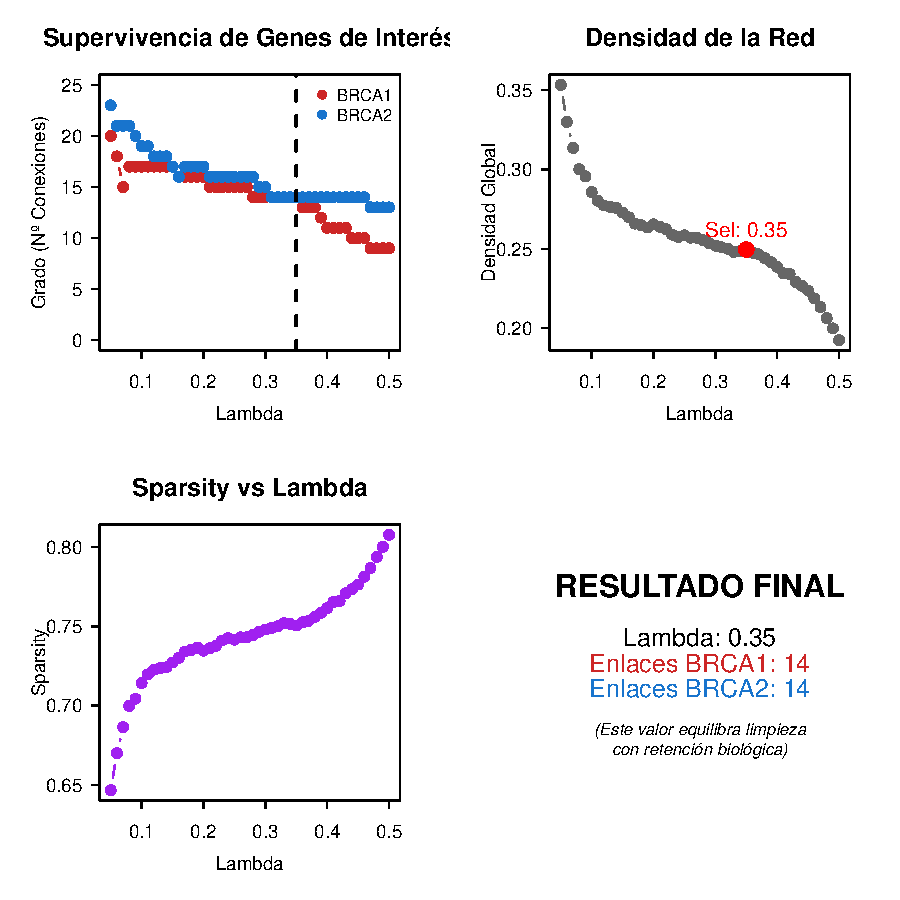
\includegraphics[width=.6\linewidth]{figure/brca1-2-Rnwunnamed-chunk-15-1} 

}


\end{knitrout}
\begin{knitrout}
\definecolor{shadecolor}{rgb}{0.969, 0.969, 0.969}\color{fgcolor}\begin{kframe}
\begin{alltt}
\hlcom{# 5.2. VISUALIZACIÓN DE REDES (SHOWCASE)}
\end{alltt}
\end{kframe}
\end{knitrout}
\begin{knitrout}
\definecolor{shadecolor}{rgb}{0.969, 0.969, 0.969}\color{fgcolor}\begin{kframe}
\begin{alltt}
\hlcom{# Muestro 3 estados: Uno laxo, el ÓPTIMO, y uno muy estricto}
\hlkwd{par}\hldef{(}\hlkwc{mfrow}\hldef{=}\hlkwd{c}\hldef{(}\hlnum{1}\hldef{,}\hlnum{3}\hldef{),} \hlkwc{mar}\hldef{=}\hlkwd{c}\hldef{(}\hlnum{2}\hldef{,}\hlnum{2}\hldef{,}\hlnum{3}\hldef{,}\hlnum{1}\hldef{))}
\hldef{lambdas_demo} \hlkwb{<-} \hlkwd{unique}\hldef{(}\hlkwd{sort}\hldef{(}\hlkwd{c}\hldef{(}\hlnum{0.1}\hldef{, best_lambda,} \hlkwd{min}\hldef{(}\hlnum{0.5}\hldef{,} \hlkwd{max}\hldef{(lambda_grid)))))}
\hlcom{# Aseguramos que el óptimo esté en el medio para comparar}
\hlkwa{if}\hldef{(}\hlkwd{length}\hldef{(lambdas_demo)} \hlopt{<} \hlnum{3}\hldef{) lambdas_demo} \hlkwb{<-} \hlkwd{c}\hldef{(lambdas_demo[}\hlnum{1}\hldef{], best_lambda, lambdas_demo[}\hlnum{2}\hldef{])}

\hlkwa{for}\hldef{(lam} \hlkwa{in} \hldef{lambdas_demo) \{}
  \hldef{idx} \hlkwb{<-} \hlkwd{which}\hldef{(metrics}\hlopt{$}\hldef{lambda} \hlopt{==} \hldef{lam)[}\hlnum{1}\hldef{]}
  \hldef{prec_temp} \hlkwb{<-} \hldef{glasso_results[[idx]]}\hlopt{$}\hldef{wi}
  \hlcom{# Recuperar nombres para el plot}
  \hlkwd{colnames}\hldef{(prec_temp)} \hlkwb{<-} \hlkwd{colnames}\hldef{(cor_tumor)}

  \hldef{titulo} \hlkwb{<-} \hlkwd{ifelse}\hldef{(lam} \hlopt{==} \hldef{best_lambda,} \hlkwd{paste}\hldef{(}\hlsng{"★ ÓPTIMO λ="}\hldef{, lam),} \hlkwd{paste}\hldef{(}\hlsng{"λ="}\hldef{, lam))}
  \hldef{color_borde} \hlkwb{<-} \hlkwd{ifelse}\hldef{(lam} \hlopt{==} \hldef{best_lambda,} \hlsng{"red"}\hldef{,} \hlsng{"black"}\hldef{)}

  \hlkwd{qgraph}\hldef{(}\hlkwd{cov2cor}\hldef{(prec_temp),}
         \hlkwc{layout}\hldef{=}\hlsng{"spring"}\hldef{,}
         \hlkwc{labels}\hldef{=}\hlkwd{colnames}\hldef{(cor_tumor),}
         \hlkwc{title}\hldef{=titulo,}
         \hlkwc{vsize}\hldef{=}\hlnum{4}\hldef{,} \hlkwc{label.cex}\hldef{=}\hlnum{0.5}\hldef{,} \hlkwc{cut}\hldef{=}\hlnum{0.01}\hldef{,} \hlkwc{legend}\hldef{=}\hlnum{FALSE}\hldef{)}
  \hlkwd{box}\hldef{(}\hlkwc{col}\hldef{=color_borde,} \hlkwc{lwd}\hldef{=}\hlkwd{ifelse}\hldef{(lam} \hlopt{==} \hldef{best_lambda,} \hlnum{3}\hldef{,} \hlnum{1}\hldef{))}
\hldef{\}}
\end{alltt}
\end{kframe}

{\centering 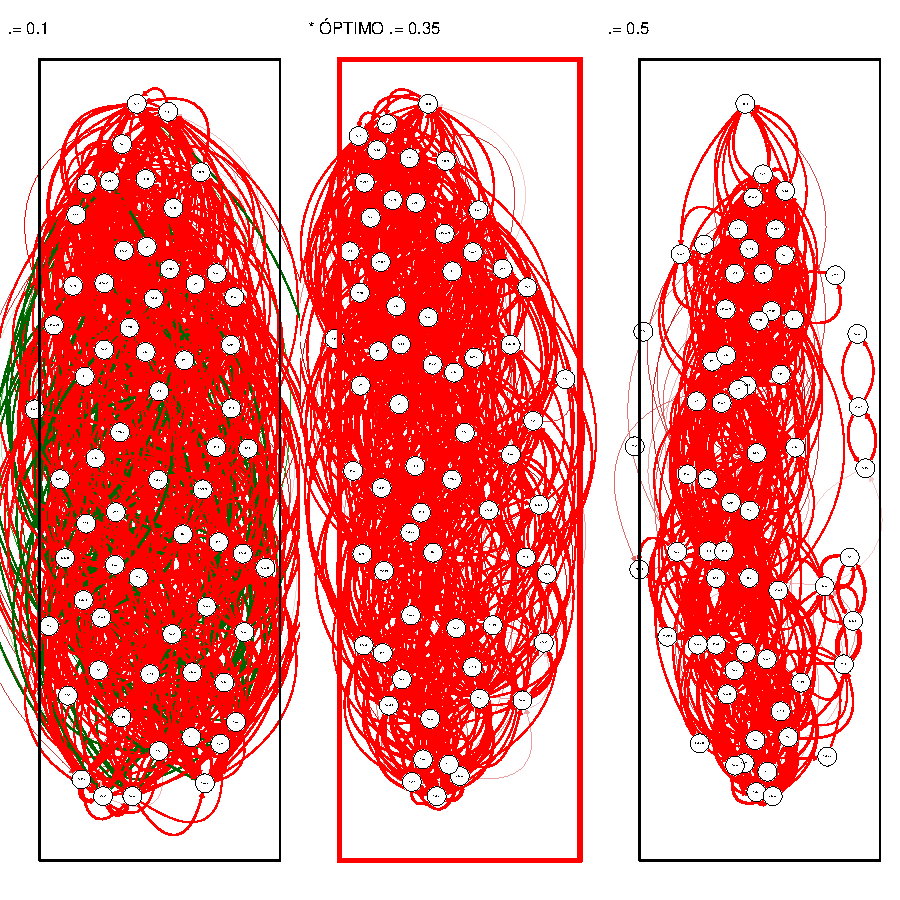
\includegraphics[width=.6\linewidth]{figure/brca1-2-Rnwunnamed-chunk-17-1} 

}


\end{knitrout}
\begin{knitrout}
\definecolor{shadecolor}{rgb}{0.969, 0.969, 0.969}\color{fgcolor}\begin{kframe}
\begin{alltt}
\hlcom{# 5.3 ASIGNACIÓN FINAL}
\end{alltt}
\end{kframe}
\end{knitrout}
\begin{knitrout}
\definecolor{shadecolor}{rgb}{0.969, 0.969, 0.969}\color{fgcolor}\begin{kframe}
\begin{alltt}
\hldef{glasso_final} \hlkwb{<-} \hldef{glasso_results[[best_idx]]}
\hldef{n_edges_final} \hlkwb{<-} \hldef{metrics}\hlopt{$}\hldef{n_edges[best_idx]}
\end{alltt}
\end{kframe}
\end{knitrout}
\begin{knitrout}
\definecolor{shadecolor}{rgb}{0.969, 0.969, 0.969}\color{fgcolor}\begin{kframe}
\begin{alltt}
\hlcom{# 6. DETECCIÓN DE COMUNIDADES}
\end{alltt}
\end{kframe}
\end{knitrout}
\begin{knitrout}
\definecolor{shadecolor}{rgb}{0.969, 0.969, 0.969}\color{fgcolor}\begin{kframe}
\begin{alltt}
\hlkwd{cat}\hldef{(}\hlsng{"\textbackslash{}n--- Detectando comunidades ---\textbackslash{}n"}\hldef{)}
\end{alltt}
\begin{verbatim}
## 
## --- Detectando comunidades ---
\end{verbatim}
\begin{alltt}
\hldef{adj} \hlkwb{<-} \hldef{(}\hlkwd{abs}\hldef{(glasso_final}\hlopt{$}\hldef{wi)} \hlopt{>} \hlnum{0.01}\hldef{)} \hlopt{*} \hlnum{1}
\hlkwd{diag}\hldef{(adj)} \hlkwb{<-} \hlnum{0}
\hldef{g} \hlkwb{<-} \hlkwd{graph_from_adjacency_matrix}\hldef{(adj,} \hlkwc{mode}\hldef{=}\hlsng{"undirected"}\hldef{)}

\hldef{communities} \hlkwb{<-} \hlkwd{cluster_louvain}\hldef{(g)}
\hldef{n_communities} \hlkwb{<-} \hlkwd{length}\hldef{(}\hlkwd{unique}\hldef{(}\hlkwd{membership}\hldef{(communities)))}
\hldef{modularity_val} \hlkwb{<-} \hlkwd{modularity}\hldef{(communities)}

\hlkwd{cat}\hldef{(}\hlkwd{sprintf}\hldef{(}\hlsng{"Comunidades detectadas: %d\textbackslash{}n"}\hldef{, n_communities))}
\end{alltt}
\begin{verbatim}
## Comunidades detectadas: 4
\end{verbatim}
\begin{alltt}
\hlkwd{cat}\hldef{(}\hlkwd{sprintf}\hldef{(}\hlsng{"Modularidad: %.3f\textbackslash{}n\textbackslash{}n"}\hldef{, modularity_val))}
\end{alltt}
\begin{verbatim}
## Modularidad: 0.330
\end{verbatim}
\begin{alltt}
\hlcom{# Mostrar composición}
\hlkwa{for}\hldef{(i} \hlkwa{in} \hlnum{1}\hlopt{:}\hldef{n_communities) \{}
  \hldef{genes_in_comm} \hlkwb{<-} \hlkwd{colnames}\hldef{(cor_tumor)[}\hlkwd{membership}\hldef{(communities)} \hlopt{==} \hldef{i]}
  \hlkwd{cat}\hldef{(}\hlkwd{sprintf}\hldef{(}\hlsng{"Comunidad %d (%d genes): %s\textbackslash{}n"}\hldef{,}
              \hldef{i,} \hlkwd{length}\hldef{(genes_in_comm),}
              \hlkwd{paste}\hldef{(genes_in_comm,} \hlkwc{collapse}\hldef{=}\hlsng{", "}\hldef{)))}
\hldef{\}}
\end{alltt}
\begin{verbatim}
## Comunidad 1 (14 genes): CREBBP, TP53BP1, SIRT1, EP300, TNKS2, RAD50, MDM2, ATM, AASDH, EMSY, ABRAXAS1, TNKS, ATR, FAN1
## Comunidad 2 (12 genes): BRCA1, MRE11, PALB2, MSH2, NBN, FANCL, MSH6, HUS1, MDC1, BARD1, TP53BP2, TOPBP1
## Comunidad 3 (21 genes): RAD51, CDC45, BABAM1, FANCE, XRCC3, SEM1, BRIP1, BRCA2, FANCI, TICRR, FANCD2, FANCC, PLK1, FEN1, RAD9A, EXO1, SFN, SHMT2, CHEK2, FANCA, FANCG
## Comunidad 4 (17 genes): MLH1, KEAP1, HSP90AA1, UIMC1, RBBP8, BCCIP, RAD51C, RPA1, TP53, BABAM2, ATRIP, ABRAXAS2, FANCF, BRCC3, MORF4L1, XRCC6, DAXX
\end{verbatim}
\begin{alltt}
\hlcom{# Colores por comunidad}
\hlkwa{if}\hldef{(n_communities} \hlopt{<=} \hlnum{8}\hldef{) \{}
  \hldef{palette_colors} \hlkwb{<-} \hlkwd{c}\hldef{(}\hlsng{"#E41A1C"}\hldef{,} \hlsng{"#377EB8"}\hldef{,} \hlsng{"#4DAF4A"}\hldef{,} \hlsng{"#984EA3"}\hldef{,}
                      \hlsng{"#FF7F00"}\hldef{,} \hlsng{"#FFFF33"}\hldef{,} \hlsng{"#A65628"}\hldef{,} \hlsng{"#F781BF"}\hldef{)}
\hldef{\}} \hlkwa{else} \hldef{\{}
  \hldef{palette_colors} \hlkwb{<-} \hlkwd{rainbow}\hldef{(n_communities,} \hlkwc{alpha}\hldef{=}\hlnum{0.8}\hldef{)}
\hldef{\}}

\hldef{node_colors} \hlkwb{<-} \hldef{palette_colors[}\hlkwd{membership}\hldef{(communities)]}
\hlkwd{names}\hldef{(node_colors)} \hlkwb{<-} \hlkwd{colnames}\hldef{(cor_tumor)}
\end{alltt}
\end{kframe}
\end{knitrout}
\begin{knitrout}
\definecolor{shadecolor}{rgb}{0.969, 0.969, 0.969}\color{fgcolor}\begin{kframe}
\begin{alltt}
\hlcom{# 7. VISUALIZACIÓN DE RED FINAL}
\end{alltt}
\end{kframe}
\end{knitrout}
\begin{knitrout}
\definecolor{shadecolor}{rgb}{0.969, 0.969, 0.969}\color{fgcolor}\begin{kframe}
\begin{alltt}
\hlkwd{cat}\hldef{(}\hlsng{"\textbackslash{}n--- Generando visualización ---\textbackslash{}n"}\hldef{)}
\end{alltt}
\begin{verbatim}
## 
## --- Generando visualización ---
\end{verbatim}
\begin{alltt}
\hlkwd{par}\hldef{(}\hlkwc{mfrow}\hldef{=}\hlkwd{c}\hldef{(}\hlnum{1}\hldef{,}\hlnum{2}\hldef{),} \hlkwc{mar}\hldef{=}\hlkwd{c}\hldef{(}\hlnum{1}\hldef{,}\hlnum{1}\hldef{,}\hlnum{3}\hldef{,}\hlnum{1}\hldef{))}

\hldef{prec_norm} \hlkwb{<-} \hlkwd{cov2cor}\hldef{(glasso_final}\hlopt{$}\hldef{wi)}
\hlkwd{diag}\hldef{(prec_norm)} \hlkwb{<-} \hlnum{0}

\hlcom{# Red con comunidades}
\hlkwd{qgraph}\hldef{(glasso_final}\hlopt{$}\hldef{wi,}
       \hlkwc{layout}\hldef{=}\hlsng{"spring"}\hldef{,}
       \hlkwc{labels}\hldef{=}\hlkwd{colnames}\hldef{(cor_tumor),}
       \hlkwc{color}\hldef{=node_colors,}
       \hlkwc{title}\hldef{=}\hlkwd{sprintf}\hldef{(}\hlsng{"Red GLASSO (λ=%.2f)\textbackslash{}n%d comunidades, %d conexiones"}\hldef{,}
                     \hldef{best_lambda, n_communities, n_edges_final),}
       \hlkwc{vsize}\hldef{=}\hlnum{7}\hldef{,}
       \hlkwc{label.cex}\hldef{=}\hlnum{0.7}\hldef{,}
       \hlkwc{cut}\hldef{=}\hlnum{0.01}\hldef{,}
       \hlkwc{legend}\hldef{=}\hlnum{FALSE}\hldef{,}
       \hlkwc{groups}\hldef{=}\hlkwd{as.factor}\hldef{(}\hlkwd{membership}\hldef{(communities)),}
       \hlkwc{diag} \hldef{=} \hlnum{FALSE}\hldef{)}

\hlcom{# 1. Librerías necesarias}
\hlkwa{if} \hldef{(}\hlopt{!}\hlkwd{require}\hldef{(}\hlsng{"ggcorrplot"}\hldef{))} \hlkwd{install.packages}\hldef{(}\hlsng{"ggcorrplot"}\hldef{)}
\end{alltt}


{\ttfamily\noindent\itshape\color{messagecolor}{\#\# Loading required package: ggcorrplot}}\begin{alltt}
\hlkwa{if} \hldef{(}\hlopt{!}\hlkwd{require}\hldef{(}\hlsng{"gridExtra"}\hldef{))} \hlkwd{install.packages}\hldef{(}\hlsng{"gridExtra"}\hldef{)} \hlcom{# Para ponerlos lado a lado}
\end{alltt}


{\ttfamily\noindent\itshape\color{messagecolor}{\#\# Loading required package: gridExtra}}

{\ttfamily\noindent\itshape\color{messagecolor}{\#\# \\\#\# Attaching package: 'gridExtra'}}

{\ttfamily\noindent\itshape\color{messagecolor}{\#\# The following object is masked from 'package:Biobase':\\\#\# \\\#\# \ \ \ \ combine}}

{\ttfamily\noindent\itshape\color{messagecolor}{\#\# The following object is masked from 'package:BiocGenerics':\\\#\# \\\#\# \ \ \ \ combine}}\begin{alltt}
\hlkwd{library}\hldef{(ggcorrplot)}
\hlkwd{library}\hldef{(gridExtra)}
\hlkwd{library}\hldef{(ggplot2)}

\hlcom{# --- 2. PREPARACIÓN DE DATOS ---}

\hlcom{# A. Matriz de Correlación (Datos Observados)}
\hldef{matriz_cor} \hlkwb{<-} \hldef{cor_tumor}

\hlcom{# B. Matriz de Precisión (Glasso -> Correlación Parcial)}
\hlcom{# Invertimos signo, normalizamos y recuperamos nombres}
\hldef{matriz_prec} \hlkwb{<-} \hlopt{-}\hlkwd{cov2cor}\hldef{(glasso_final}\hlopt{$}\hldef{wi)}
\hlkwd{diag}\hldef{(matriz_prec)} \hlkwb{<-} \hlnum{1}
\hlkwd{rownames}\hldef{(matriz_prec)} \hlkwb{<-} \hlkwd{rownames}\hldef{(cor_tumor)}
\hlkwd{colnames}\hldef{(matriz_prec)} \hlkwb{<-} \hlkwd{colnames}\hldef{(cor_tumor)}

\hlcom{# --- 3. GENERACIÓN DE GRÁFICOS ---}

\hlcom{# GRÁFICO 1: Correlación Estándar (Escala normal -1 a 1)}
\hldef{plot_cor} \hlkwb{<-} \hlkwd{ggcorrplot}\hldef{(matriz_cor,}
                       \hlkwc{method} \hldef{=} \hlsng{"square"}\hldef{,}
                       \hlkwc{type} \hldef{=} \hlsng{"lower"}\hldef{,}
                       \hlkwc{lab} \hldef{=} \hlnum{FALSE}\hldef{,}          \hlcom{# Sin números}
                       \hlkwc{show.diag} \hldef{=} \hlnum{FALSE}\hldef{,}    \hlcom{# Ocultar diagonal (opcional, limpia más)}
                       \hlkwc{colors} \hldef{=} \hlkwd{c}\hldef{(}\hlsng{"navy"}\hldef{,} \hlsng{"white"}\hldef{,} \hlsng{"firebrick3"}\hldef{),}
                       \hlkwc{title} \hldef{=} \hlsng{"Correlación (Pearson)"}\hldef{,}
                       \hlkwc{tl.cex} \hldef{=} \hlnum{9}
\hldef{)} \hlopt{+} \hlkwd{theme}\hldef{(}\hlkwc{legend.position} \hldef{=} \hlsng{"bottom"}\hldef{)} \hlcom{# Leyenda abajo para ahorrar espacio lateral}
\end{alltt}


{\ttfamily\noindent\color{warningcolor}{\#\# Warning: `aes\_string()` was deprecated in ggplot2 3.0.0.\\\#\# i Please use tidy evaluation idioms with `aes()`.\\\#\# i See also `vignette("{}ggplot2-in-packages"{})` for more information.\\\#\# i The deprecated feature was likely used in the ggcorrplot package.\\\#\# \ \ Please report the issue at <https://github.com/kassambara/ggcorrplot/issues>.\\\#\# This warning is displayed once every 8 hours.\\\#\# Call `lifecycle::last\_lifecycle\_warnings()` to see where this warning was generated.}}\begin{alltt}
\hlcom{# GRÁFICO 2: Precisión Glasso (Escala ajustada -0.5 a 0.5)}
\hldef{plot_prec} \hlkwb{<-} \hlkwd{ggcorrplot}\hldef{(matriz_prec,}
                        \hlkwc{method} \hldef{=} \hlsng{"square"}\hldef{,}
                        \hlkwc{type} \hldef{=} \hlsng{"lower"}\hldef{,}
                        \hlkwc{lab} \hldef{=} \hlnum{FALSE}\hldef{,}
                        \hlkwc{show.diag} \hldef{=} \hlnum{FALSE}\hldef{,}
                        \hlkwc{title} \hldef{=} \hlsng{"Correlación Parcial (Glasso)"}\hldef{,}
                        \hlkwc{tl.cex} \hldef{=} \hlnum{9}
\hldef{)} \hlopt{+}
  \hlcom{# AQUÍ ESTÁ EL TRUCO DE LA ESCALA:}
  \hlcom{# Sobreescribimos la escala de color por defecto de ggcorrplot}
  \hlcom{# 'limit = c(-0.5, 0.5)' hace que todo lo que pase de 0.5 sea rojo puro}
  \hlcom{# 'oob = scales::squish' asegura que no de error si hay valores mayores}
  \hlkwd{scale_fill_gradient2}\hldef{(}\hlkwc{low} \hldef{=} \hlsng{"navy"}\hldef{,} \hlkwc{high} \hldef{=} \hlsng{"firebrick3"}\hldef{,} \hlkwc{mid} \hldef{=} \hlsng{"white"}\hldef{,}
                       \hlkwc{midpoint} \hldef{=} \hlnum{0}\hldef{,} \hlkwc{limit} \hldef{=} \hlkwd{c}\hldef{(}\hlopt{-}\hlnum{0.25}\hldef{,} \hlnum{0.25}\hldef{),}
                       \hlkwc{space} \hldef{=} \hlsng{"Lab"}\hldef{,} \hlkwc{name} \hldef{=} \hlsng{"Corr"}\hldef{)} \hlopt{+}
  \hlkwd{theme}\hldef{(}\hlkwc{legend.position} \hldef{=} \hlsng{"bottom"}\hldef{)}
\end{alltt}


{\ttfamily\noindent\itshape\color{messagecolor}{\#\# Scale for fill is already present.\\\#\# Adding another scale for fill, which will replace the existing scale.}}\begin{alltt}
\hlcom{# --- 4. VISUALIZACIÓN FINAL ---}

\hlcom{# Mostramos ambos gráficos en una misma ventana (1 fila, 2 columnas)}
\hlkwd{grid.arrange}\hldef{(plot_cor, plot_prec,} \hlkwc{ncol} \hldef{=} \hlnum{2}\hldef{)}
\end{alltt}
\end{kframe}

{\centering 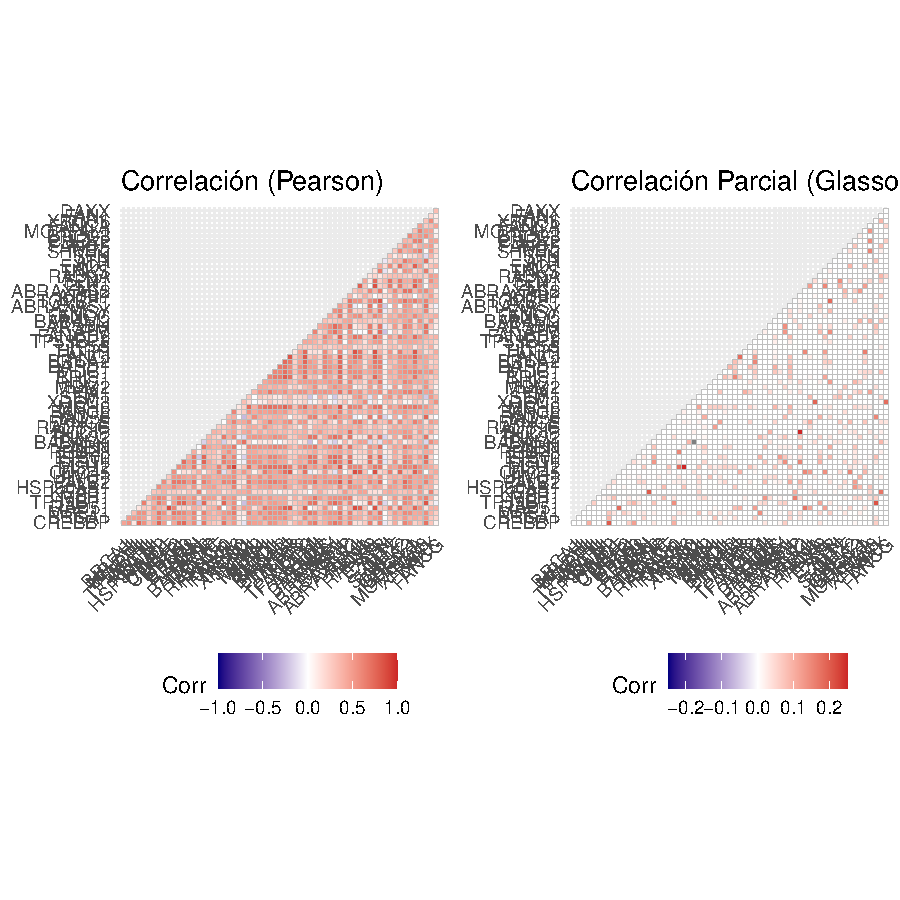
\includegraphics[width=.6\linewidth]{figure/brca1-2-Rnwunnamed-chunk-23-1} 

}


\end{knitrout}
\begin{knitrout}
\definecolor{shadecolor}{rgb}{0.969, 0.969, 0.969}\color{fgcolor}\begin{kframe}
\begin{alltt}
\hlcom{# 8. ANÁLISIS DE VECINDARIOS DE BRCA1/2}
\end{alltt}
\end{kframe}
\end{knitrout}
\begin{knitrout}
\definecolor{shadecolor}{rgb}{0.969, 0.969, 0.969}\color{fgcolor}\begin{kframe}
\begin{alltt}
\hlkwd{cat}\hldef{(}\hlsng{"\textbackslash{}n========== VECINDARIOS DE BRCA1/2 ==========\textbackslash{}n"}\hldef{)}
\end{alltt}
\begin{verbatim}
## 
## ========== VECINDARIOS DE BRCA1/2 ==========
\end{verbatim}
\begin{alltt}
\hldef{matriz_precision_final} \hlkwb{<-} \hldef{glasso_final}\hlopt{$}\hldef{wi}
\hlkwd{rownames}\hldef{(matriz_precision_final)} \hlkwb{<-} \hlkwd{rownames}\hldef{(cor_tumor)}
\hlkwd{colnames}\hldef{(matriz_precision_final)} \hlkwb{<-} \hlkwd{colnames}\hldef{(cor_tumor)}

\hldef{analyze_neighborhood} \hlkwb{<-} \hlkwa{function}\hldef{(}\hlkwc{gene_name}\hldef{,} \hlkwc{precision_matrix}\hldef{,} \hlkwc{top_n}\hldef{=}\hlnum{10}\hldef{) \{}
  \hlkwa{if}\hldef{(}\hlopt{!}\hldef{gene_name} \hlopt{%in%} \hlkwd{colnames}\hldef{(precision_matrix)) \{}
    \hlkwd{cat}\hldef{(}\hlkwd{sprintf}\hldef{(}\hlsng{"  %s no encontrado\textbackslash{}n"}\hldef{, gene_name))}
    \hlkwd{return}\hldef{(}\hlkwa{NULL}\hldef{)}
  \hldef{\}}

  \hldef{gene_idx} \hlkwb{<-} \hlkwd{which}\hldef{(}\hlkwd{colnames}\hldef{(precision_matrix)} \hlopt{==} \hldef{gene_name)}
  \hldef{connections} \hlkwb{<-} \hldef{precision_matrix[gene_idx, ]}
  \hldef{connections} \hlkwb{<-} \hldef{connections[}\hlkwd{names}\hldef{(connections)} \hlopt{!=} \hldef{gene_name]}

  \hldef{connections_sorted} \hlkwb{<-} \hlkwd{sort}\hldef{(}\hlkwd{abs}\hldef{(connections),} \hlkwc{decreasing}\hldef{=}\hlnum{TRUE}\hldef{)}
  \hldef{top_connections} \hlkwb{<-} \hldef{connections_sorted[}\hlnum{1}\hlopt{:}\hlkwd{min}\hldef{(top_n,} \hlkwd{length}\hldef{(connections_sorted))]}
  \hldef{original_signs} \hlkwb{<-} \hlkwd{sign}\hldef{(connections[}\hlkwd{names}\hldef{(top_connections)])}

  \hlkwd{return}\hldef{(}\hlkwd{list}\hldef{(}
    \hlkwc{neighbors} \hldef{=} \hlkwd{names}\hldef{(top_connections),}
    \hlkwc{strengths} \hldef{= top_connections,}
    \hlkwc{signs} \hldef{= original_signs}
  \hldef{))}
\hldef{\}}

\hlcom{# BRCA1}
\hlkwd{cat}\hldef{(}\hlsng{"\textbackslash{}n--- BRCA1 ---\textbackslash{}n"}\hldef{)}
\end{alltt}
\begin{verbatim}
## 
## --- BRCA1 ---
\end{verbatim}
\begin{alltt}
\hldef{brca1_neighbors} \hlkwb{<-} \hlkwd{analyze_neighborhood}\hldef{(}\hlsng{"BRCA1"}\hldef{, matriz_precision_final,} \hlkwc{top_n}\hldef{=}\hlnum{10}\hldef{)}

\hlkwa{if}\hldef{(}\hlopt{!}\hlkwd{is.null}\hldef{(brca1_neighbors)} \hlopt{&&} \hlkwd{length}\hldef{(brca1_neighbors}\hlopt{$}\hldef{neighbors)} \hlopt{>} \hlnum{0}\hldef{) \{}
  \hlkwd{cat}\hldef{(}\hlsng{"Top 10 vecinos directos:\textbackslash{}n"}\hldef{)}
  \hlkwa{for}\hldef{(i} \hlkwa{in} \hlnum{1}\hlopt{:}\hlkwd{length}\hldef{(brca1_neighbors}\hlopt{$}\hldef{neighbors)) \{}
    \hldef{sign_str} \hlkwb{<-} \hlkwd{ifelse}\hldef{(brca1_neighbors}\hlopt{$}\hldef{signs[i]} \hlopt{>} \hlnum{0}\hldef{,} \hlsng{"+"}\hldef{,} \hlsng{"-"}\hldef{)}
    \hlkwd{cat}\hldef{(}\hlkwd{sprintf}\hldef{(}\hlsng{"  %2d. %-12s (fuerza: %.4f, dirección: %s)\textbackslash{}n"}\hldef{,}
                \hldef{i, brca1_neighbors}\hlopt{$}\hldef{neighbors[i],}
                \hldef{brca1_neighbors}\hlopt{$}\hldef{strengths[i], sign_str))}
  \hldef{\}}
\hldef{\}} \hlkwa{else} \hldef{\{}
  \hlkwd{cat}\hldef{(}\hlsng{"  Sin vecinos significativos\textbackslash{}n"}\hldef{)}
\hldef{\}}
\end{alltt}
\begin{verbatim}
## Top 10 vecinos directos:
##    1. PALB2        (fuerza: 0.1210, dirección: -)
##    2. BRIP1        (fuerza: 0.0906, dirección: -)
##    3. FANCD2       (fuerza: 0.0810, dirección: -)
##    4. TOPBP1       (fuerza: 0.0807, dirección: -)
##    5. RAD50        (fuerza: 0.0659, dirección: -)
##    6. NBN          (fuerza: 0.0639, dirección: -)
##    7. FANCI        (fuerza: 0.0621, dirección: -)
##    8. FAN1         (fuerza: 0.0486, dirección: -)
##    9. ABRAXAS2     (fuerza: 0.0425, dirección: -)
##   10. BARD1        (fuerza: 0.0217, dirección: -)
\end{verbatim}
\begin{alltt}
\hlcom{# BRCA2}
\hlkwd{cat}\hldef{(}\hlsng{"\textbackslash{}n--- BRCA2 ---\textbackslash{}n"}\hldef{)}
\end{alltt}
\begin{verbatim}
## 
## --- BRCA2 ---
\end{verbatim}
\begin{alltt}
\hldef{brca2_neighbors} \hlkwb{<-} \hlkwd{analyze_neighborhood}\hldef{(}\hlsng{"BRCA2"}\hldef{, matriz_precision_final,} \hlkwc{top_n}\hldef{=}\hlnum{10}\hldef{)}

\hlkwa{if}\hldef{(}\hlopt{!}\hlkwd{is.null}\hldef{(brca2_neighbors)} \hlopt{&&} \hlkwd{length}\hldef{(brca2_neighbors}\hlopt{$}\hldef{neighbors)} \hlopt{>} \hlnum{0}\hldef{) \{}
  \hlkwd{cat}\hldef{(}\hlsng{"Top 10 vecinos directos:\textbackslash{}n"}\hldef{)}
  \hlkwa{for}\hldef{(i} \hlkwa{in} \hlnum{1}\hlopt{:}\hlkwd{length}\hldef{(brca2_neighbors}\hlopt{$}\hldef{neighbors)) \{}
    \hldef{sign_str} \hlkwb{<-} \hlkwd{ifelse}\hldef{(brca2_neighbors}\hlopt{$}\hldef{signs[i]} \hlopt{>} \hlnum{0}\hldef{,} \hlsng{"+"}\hldef{,} \hlsng{"-"}\hldef{)}
    \hlkwd{cat}\hldef{(}\hlkwd{sprintf}\hldef{(}\hlsng{"  %2d. %-12s (fuerza: %.4f, dirección: %s)\textbackslash{}n"}\hldef{,}
                \hldef{i, brca2_neighbors}\hlopt{$}\hldef{neighbors[i],}
                \hldef{brca2_neighbors}\hlopt{$}\hldef{strengths[i], sign_str))}
  \hldef{\}}
\hldef{\}} \hlkwa{else} \hldef{\{}
  \hlkwd{cat}\hldef{(}\hlsng{"  Sin vecinos significativos\textbackslash{}n"}\hldef{)}
\hldef{\}}
\end{alltt}
\begin{verbatim}
## Top 10 vecinos directos:
##    1. FANCD2       (fuerza: 0.2257, dirección: -)
##    2. FANCI        (fuerza: 0.1198, dirección: -)
##    3. BARD1        (fuerza: 0.1191, dirección: -)
##    4. TOPBP1       (fuerza: 0.1037, dirección: -)
##    5. EXO1         (fuerza: 0.0939, dirección: -)
##    6. ATR          (fuerza: 0.0914, dirección: -)
##    7. FANCA        (fuerza: 0.0888, dirección: -)
##    8. MSH2         (fuerza: 0.0600, dirección: -)
##    9. BRIP1        (fuerza: 0.0544, dirección: -)
##   10. NBN          (fuerza: 0.0520, dirección: -)
\end{verbatim}
\begin{alltt}
\hlcom{# Overlap entre BRCA1 y BRCA2}
\hlkwa{if}\hldef{(}\hlopt{!}\hlkwd{is.null}\hldef{(brca1_neighbors)} \hlopt{&& !}\hlkwd{is.null}\hldef{(brca2_neighbors)) \{}
  \hldef{common_neighbors} \hlkwb{<-} \hlkwd{intersect}\hldef{(brca1_neighbors}\hlopt{$}\hldef{neighbors, brca2_neighbors}\hlopt{$}\hldef{neighbors)}
  \hlkwa{if}\hldef{(}\hlkwd{length}\hldef{(common_neighbors)} \hlopt{>} \hlnum{0}\hldef{) \{}
    \hlkwd{cat}\hldef{(}\hlsng{"\textbackslash{}nVecinos compartidos por BRCA1 y BRCA2:\textbackslash{}n"}\hldef{)}
    \hlkwd{cat}\hldef{(}\hlsng{" "}\hldef{,} \hlkwd{paste}\hldef{(common_neighbors,} \hlkwc{collapse}\hldef{=}\hlsng{", "}\hldef{),} \hlsng{"\textbackslash{}n"}\hldef{)}
  \hldef{\}}
\hldef{\}}
\end{alltt}
\begin{verbatim}
## 
## Vecinos compartidos por BRCA1 y BRCA2:
##   BRIP1, FANCD2, TOPBP1, NBN, FANCI, BARD1
\end{verbatim}
\end{kframe}
\end{knitrout}
\begin{knitrout}
\definecolor{shadecolor}{rgb}{0.969, 0.969, 0.969}\color{fgcolor}\begin{kframe}
\begin{alltt}
\hlcom{# 9. ANÁLISIS DE ESTABILIDAD DE VECINDARIOS}
\end{alltt}
\end{kframe}
\end{knitrout}
\begin{knitrout}
\definecolor{shadecolor}{rgb}{0.969, 0.969, 0.969}\color{fgcolor}\begin{kframe}
\begin{alltt}
\hlkwd{cat}\hldef{(}\hlsng{"\textbackslash{}n========== ESTABILIDAD DE VECINDARIOS ==========\textbackslash{}n"}\hldef{)}
\end{alltt}
\begin{verbatim}
## 
## ========== ESTABILIDAD DE VECINDARIOS ==========
\end{verbatim}
\begin{alltt}
\hlkwd{cat}\hldef{(}\hlsng{"(Analizando cómo cambian con lambda)\textbackslash{}n\textbackslash{}n"}\hldef{)}
\end{alltt}
\begin{verbatim}
## (Analizando cómo cambian con lambda)
\end{verbatim}
\begin{alltt}
\hlcom{# Para BRCA1, ver vecinos en diferentes lambdas}
\hldef{lambda_stability} \hlkwb{<-} \hlkwd{c}\hldef{(}\hlnum{0.15}\hldef{,} \hlnum{0.25}\hldef{,} \hlnum{0.35}\hldef{, best_lambda)}

\hlkwd{cat}\hldef{(}\hlsng{"--- Estabilidad de vecinos de BRCA1 ---\textbackslash{}n"}\hldef{)}
\end{alltt}
\begin{verbatim}
## --- Estabilidad de vecinos de BRCA1 ---
\end{verbatim}
\begin{alltt}
\hldef{brca1_stability} \hlkwb{<-} \hlkwd{list}\hldef{()}

\hlkwa{for}\hldef{(lam} \hlkwa{in} \hldef{lambda_stability) \{}
  \hldef{idx} \hlkwb{<-} \hlkwd{which.min}\hldef{(}\hlkwd{abs}\hldef{(lambda_grid} \hlopt{-} \hldef{lam))}
  \hldef{neighbors} \hlkwb{<-} \hlkwd{analyze_neighborhood}\hldef{(}\hlsng{"BRCA1"}\hldef{, matriz_precision_final,} \hlkwc{top_n}\hldef{=}\hlnum{5}\hldef{)}

  \hlkwa{if}\hldef{(}\hlopt{!}\hlkwd{is.null}\hldef{(neighbors)) \{}
    \hldef{brca1_stability[[}\hlkwd{as.character}\hldef{(lam)]]} \hlkwb{<-} \hldef{neighbors}\hlopt{$}\hldef{neighbors}
    \hlkwd{cat}\hldef{(}\hlkwd{sprintf}\hldef{(}\hlsng{"\textbackslash{}nλ=%.2f: %s\textbackslash{}n"}\hldef{, lam,} \hlkwd{paste}\hldef{(neighbors}\hlopt{$}\hldef{neighbors,} \hlkwc{collapse}\hldef{=}\hlsng{", "}\hldef{)))}
  \hldef{\}}
\hldef{\}}
\end{alltt}
\begin{verbatim}
## 
## λ=0.15: PALB2, BRIP1, FANCD2, TOPBP1, RAD50
## 
## λ=0.25: PALB2, BRIP1, FANCD2, TOPBP1, RAD50
## 
## λ=0.35: PALB2, BRIP1, FANCD2, TOPBP1, RAD50
## 
## λ=0.35: PALB2, BRIP1, FANCD2, TOPBP1, RAD50
\end{verbatim}
\begin{alltt}
\hlcom{# Genes que aparecen en todos los lambdas (estables)}
\hlkwa{if}\hldef{(}\hlkwd{length}\hldef{(brca1_stability)} \hlopt{>} \hlnum{0}\hldef{) \{}
  \hldef{stable_neighbors} \hlkwb{<-} \hlkwd{Reduce}\hldef{(intersect, brca1_stability)}
  \hlkwd{cat}\hldef{(}\hlsng{"\textbackslash{}nVecinos ESTABLES de BRCA1 (en todos los lambdas):\textbackslash{}n"}\hldef{)}
  \hlkwa{if}\hldef{(}\hlkwd{length}\hldef{(stable_neighbors)} \hlopt{>} \hlnum{0}\hldef{) \{}
    \hlkwd{cat}\hldef{(}\hlsng{" "}\hldef{,} \hlkwd{paste}\hldef{(stable_neighbors,} \hlkwc{collapse}\hldef{=}\hlsng{", "}\hldef{),} \hlsng{"\textbackslash{}n"}\hldef{)}
  \hldef{\}} \hlkwa{else} \hldef{\{}
    \hlkwd{cat}\hldef{(}\hlsng{"  Ninguno (los vecindarios varían con lambda)\textbackslash{}n"}\hldef{)}
  \hldef{\}}
\hldef{\}}
\end{alltt}
\begin{verbatim}
## 
## Vecinos ESTABLES de BRCA1 (en todos los lambdas):
##   PALB2, BRIP1, FANCD2, TOPBP1, RAD50
\end{verbatim}
\end{kframe}
\end{knitrout}
\begin{knitrout}
\definecolor{shadecolor}{rgb}{0.969, 0.969, 0.969}\color{fgcolor}\begin{kframe}
\begin{alltt}
\hlcom{# 10. MÉTRICAS AVANZADAS DE RED}
\end{alltt}
\end{kframe}
\end{knitrout}
\begin{knitrout}
\definecolor{shadecolor}{rgb}{0.969, 0.969, 0.969}\color{fgcolor}\begin{kframe}
\begin{alltt}
\hlkwd{library}\hldef{(igraph)}

\hlkwd{cat}\hldef{(}\hlsng{"\textbackslash{}n========== MÉTRICAS DE RED (TOPOLOGÍA GLASSO) ==========\textbackslash{}n"}\hldef{)}
\end{alltt}
\begin{verbatim}
## 
## ========== MÉTRICAS DE RED (TOPOLOGÍA GLASSO) ==========
\end{verbatim}
\begin{alltt}
\hlcom{# 1. Crear objeto grafo desde tu matriz limpia}
\hlcom{# Usamos 'matriz_precision_final' (la que tiene nombres)}
\hlcom{# Convertimos a adyacencia: 1 si hay conexión, 0 si no (binario)}
\hldef{adj_matrix} \hlkwb{<-} \hldef{matriz_precision_final} \hlopt{!=} \hlnum{0}
\hlkwd{diag}\hldef{(adj_matrix)} \hlkwb{<-} \hlnum{0} \hlcom{# Sin auto-bucles}
\hldef{g} \hlkwb{<-} \hlkwd{graph_from_adjacency_matrix}\hldef{(adj_matrix,} \hlkwc{mode} \hldef{=} \hlsng{"undirected"}\hldef{)}

\hlcom{# 2. Calcular Métricas Clave}
\hldef{grados} \hlkwb{<-} \hlkwd{degree}\hldef{(g)}
\hldef{betweenness} \hlkwb{<-} \hlkwd{betweenness}\hldef{(g,} \hlkwc{normalized} \hldef{=} \hlnum{TRUE}\hldef{)}

\hlcom{# 3. Crear Dataframe de Importancia}
\hldef{df_metrics} \hlkwb{<-} \hlkwd{data.frame}\hldef{(}
  \hlkwc{Gen} \hldef{=} \hlkwd{names}\hldef{(grados),}
  \hlkwc{Grado} \hldef{= grados,}
  \hlkwc{Intermediacion} \hldef{= betweenness}
\hldef{)}

\hlcom{# Ordenar por Grado (Hubs)}
\hldef{top_hubs} \hlkwb{<-} \hldef{df_metrics[}\hlkwd{order}\hldef{(df_metrics}\hlopt{$}\hldef{Grado,} \hlkwc{decreasing} \hldef{=} \hlnum{TRUE}\hldef{), ][}\hlnum{1}\hlopt{:}\hlnum{10}\hldef{, ]}

\hlcom{# Ordenar por Intermediación (Puentes)}
\hldef{top_bridges} \hlkwb{<-} \hldef{df_metrics[}\hlkwd{order}\hldef{(df_metrics}\hlopt{$}\hldef{Intermediacion,} \hlkwc{decreasing} \hldef{=} \hlnum{TRUE}\hldef{), ][}\hlnum{1}\hlopt{:}\hlnum{10}\hldef{, ]}

\hlkwd{cat}\hldef{(}\hlsng{"--- Top 10 Hubs (Mayor conectividad directa) ---\textbackslash{}n"}\hldef{)}
\end{alltt}
\begin{verbatim}
## --- Top 10 Hubs (Mayor conectividad directa) ---
\end{verbatim}
\begin{alltt}
\hlkwd{print}\hldef{(top_hubs[,} \hlkwd{c}\hldef{(}\hlsng{"Gen"}\hldef{,} \hlsng{"Grado"}\hldef{)])}
\end{alltt}
\begin{verbatim}
##               Gen Grado
## MSH6         MSH6    27
## PALB2       PALB2    26
## TOPBP1     TOPBP1    26
## MRE11       MRE11    24
## MLH1         MLH1    24
## RPA1         RPA1    23
## ABRAXAS2 ABRAXAS2    23
## SIRT1       SIRT1    22
## FEN1         FEN1    22
## UIMC1       UIMC1    21
\end{verbatim}
\begin{alltt}
\hlkwd{cat}\hldef{(}\hlsng{"\textbackslash{}n--- Top 10 Puentes (Mayor flujo de información) ---\textbackslash{}n"}\hldef{)}
\end{alltt}
\begin{verbatim}
## 
## --- Top 10 Puentes (Mayor flujo de información) ---
\end{verbatim}
\begin{alltt}
\hlkwd{print}\hldef{(top_bridges[,} \hlkwd{c}\hldef{(}\hlsng{"Gen"}\hldef{,} \hlsng{"Intermediacion"}\hldef{)])}
\end{alltt}
\begin{verbatim}
##           Gen Intermediacion
## FEN1     FEN1     0.05469652
## RPA1     RPA1     0.05321936
## DAXX     DAXX     0.04987723
## MSH6     MSH6     0.04289592
## MLH1     MLH1     0.04134319
## UIMC1   UIMC1     0.03874789
## PALB2   PALB2     0.03526490
## MDC1     MDC1     0.03229718
## XRCC6   XRCC6     0.03126776
## TOPBP1 TOPBP1     0.02735748
\end{verbatim}
\begin{alltt}
\hlcom{# 4. Ver específicamente BRCA1}
\hlkwa{if}\hldef{(}\hlsng{"BRCA1"} \hlopt{%in%} \hldef{df_metrics}\hlopt{$}\hldef{Gen) \{}
  \hlkwd{cat}\hldef{(}\hlsng{"\textbackslash{}n--- Métricas BRCA1 ---\textbackslash{}n"}\hldef{)}
  \hlkwd{print}\hldef{(df_metrics[df_metrics}\hlopt{$}\hldef{Gen} \hlopt{==} \hlsng{"BRCA1"}\hldef{, ])}
\hldef{\}}
\end{alltt}
\begin{verbatim}
## 
## --- Métricas BRCA1 ---
##         Gen Grado Intermediacion
## BRCA1 BRCA1    14     0.02061227
\end{verbatim}
\begin{alltt}
\hlcom{# 5. Ver específicamente BRCA2}
\hlkwa{if}\hldef{(}\hlsng{"BRCA2"} \hlopt{%in%} \hldef{df_metrics}\hlopt{$}\hldef{Gen) \{}
  \hlkwd{cat}\hldef{(}\hlsng{"\textbackslash{}n--- Métricas BRCA2 ---\textbackslash{}n"}\hldef{)}
  \hlkwd{print}\hldef{(df_metrics[df_metrics}\hlopt{$}\hldef{Gen} \hlopt{==} \hlsng{"BRCA2"}\hldef{, ])}
\hldef{\}}
\end{alltt}
\begin{verbatim}
## 
## --- Métricas BRCA2 ---
##         Gen Grado Intermediacion
## BRCA2 BRCA2    14    0.008947296
\end{verbatim}
\end{kframe}
\end{knitrout}
\begin{knitrout}
\definecolor{shadecolor}{rgb}{0.969, 0.969, 0.969}\color{fgcolor}\begin{kframe}
\begin{alltt}
\hlcom{# 11. VALIDACIÓN CON STRING}
\end{alltt}
\end{kframe}
\end{knitrout}
\begin{knitrout}
\definecolor{shadecolor}{rgb}{0.969, 0.969, 0.969}\color{fgcolor}\begin{kframe}
\begin{alltt}
\hlkwd{cat}\hldef{(}\hlsng{"========== VALIDACIÓN INTEGRAL: STRING vs TCGA vs GLASSO ==========\textbackslash{}n"}\hldef{)}
\end{alltt}
\begin{verbatim}
## ========== VALIDACIÓN INTEGRAL: STRING vs TCGA vs GLASSO ==========
\end{verbatim}
\end{kframe}
\end{knitrout}
\begin{knitrout}
\definecolor{shadecolor}{rgb}{0.969, 0.969, 0.969}\color{fgcolor}\begin{kframe}
\begin{alltt}
\hlcom{# 11.1. CARGAR DATOS (CON CORRECCIÓN DPLYR)}
\end{alltt}
\end{kframe}
\end{knitrout}
\begin{knitrout}
\definecolor{shadecolor}{rgb}{0.969, 0.969, 0.969}\color{fgcolor}\begin{kframe}
\begin{alltt}
\hldef{file_string} \hlkwb{<-} \hlsng{"brca_ego_network_data.csv"}
\hlkwa{if}\hldef{(}\hlopt{!}\hlkwd{file.exists}\hldef{(file_string))} \hlkwd{stop}\hldef{(}\hlsng{"Falta el archivo CSV de STRING."}\hldef{)}

\hldef{df_string} \hlkwb{<-} \hlkwd{read.csv}\hldef{(file_string,} \hlkwc{stringsAsFactors} \hldef{=} \hlnum{FALSE}\hldef{)}

\hlcom{# --- CORRECCIÓN AQUÍ: Usamos dplyr::select para evitar el error ---}
\hldef{df_edges} \hlkwb{<-} \hldef{df_string} \hlopt{%>%}
  \hlkwd{filter}\hldef{(origin_gene} \hlopt{!=} \hlsng{"SEED"} \hlopt{&} \hldef{origin_gene} \hlopt{!=} \hlsng{"From_Step1"}\hldef{)} \hlopt{%>%}
  \hldef{dplyr}\hlopt{::}\hlkwd{select}\hldef{(}\hlkwc{GenA} \hldef{= origin_gene,} \hlkwc{GenB} \hldef{= gene_symbol,} \hlkwc{STRING_Score} \hldef{= score)}
\end{alltt}


{\ttfamily\noindent\bfseries\color{errorcolor}{\#\# Error: object 'origin\_gene' not found}}\begin{alltt}
\hlcom{# ID único ordenado}
\hldef{df_edges}\hlopt{$}\hldef{PairID} \hlkwb{<-} \hlkwd{apply}\hldef{(df_edges[,} \hlkwd{c}\hldef{(}\hlsng{"GenA"}\hldef{,} \hlsng{"GenB"}\hldef{)],} \hlnum{1}\hldef{,} \hlkwa{function}\hldef{(}\hlkwc{x}\hldef{)} \hlkwd{paste}\hldef{(}\hlkwd{sort}\hldef{(x),} \hlkwc{collapse} \hldef{=} \hlsng{"_"}\hldef{))}
\end{alltt}


{\ttfamily\noindent\bfseries\color{errorcolor}{\#\# Error: object 'df\_edges' not found}}\begin{alltt}
\hlkwd{cat}\hldef{(}\hlkwd{sprintf}\hldef{(}\hlsng{"Conexiones de STRING cargadas: %d\textbackslash{}n"}\hldef{,} \hlkwd{nrow}\hldef{(df_edges)))}
\end{alltt}


{\ttfamily\noindent\bfseries\color{errorcolor}{\#\# Error in h(simpleError(msg, call)): error in evaluating the argument 'x' in selecting a method for function 'nrow': object 'df\_edges' not found}}\end{kframe}
\end{knitrout}
\begin{knitrout}
\definecolor{shadecolor}{rgb}{0.969, 0.969, 0.969}\color{fgcolor}\begin{kframe}
\begin{alltt}
\hlcom{# 11.2. CRUZAR CON TUS DATOS (TCGA & GLASSO)}
\end{alltt}
\end{kframe}
\end{knitrout}
\begin{knitrout}
\definecolor{shadecolor}{rgb}{0.969, 0.969, 0.969}\color{fgcolor}\begin{kframe}
\begin{alltt}
\hlcom{# A. Mapear Pearson (TCGA)}
\end{alltt}
\end{kframe}
\end{knitrout}
\begin{knitrout}
\definecolor{shadecolor}{rgb}{0.969, 0.969, 0.969}\color{fgcolor}\begin{kframe}
\begin{alltt}
\hldef{get_pearson} \hlkwb{<-} \hlkwa{function}\hldef{(}\hlkwc{g1}\hldef{,} \hlkwc{g2}\hldef{,} \hlkwc{mat}\hldef{) \{}
  \hlkwa{if}\hldef{(g1} \hlopt{%in%} \hlkwd{rownames}\hldef{(mat)} \hlopt{&&} \hldef{g2} \hlopt{%in%} \hlkwd{rownames}\hldef{(mat))} \hlkwd{return}\hldef{(mat[g1, g2])}
  \hlkwa{else} \hlkwd{return}\hldef{(}\hlnum{NA}\hldef{)}
\hldef{\}}
\hldef{df_edges}\hlopt{$}\hldef{Pearson_TCGA} \hlkwb{<-} \hlkwd{mapply}\hldef{(get_pearson, df_edges}\hlopt{$}\hldef{GenA, df_edges}\hlopt{$}\hldef{GenB,} \hlkwc{MoreArgs} \hldef{=} \hlkwd{list}\hldef{(}\hlkwc{mat} \hldef{= cor_tumor))}
\end{alltt}


{\ttfamily\noindent\bfseries\color{errorcolor}{\#\# Error: object 'df\_edges' not found}}\begin{alltt}
\hlcom{# B. Mapear Glasso (Lambda Óptimo)}
\end{alltt}
\end{kframe}
\end{knitrout}
\begin{knitrout}
\definecolor{shadecolor}{rgb}{0.969, 0.969, 0.969}\color{fgcolor}\begin{kframe}
\begin{alltt}
\hlcom{# Aseguramos tener la matriz parcial lista (Lambda 0.35 según tu elección)}
\hldef{lambda_best} \hlkwb{<-} \hldef{best_lambda}
\hlkwa{if}\hldef{(}\hlopt{!}\hlkwd{exists}\hldef{(}\hlsng{"partial_corr"}\hldef{)) \{}
  \hlkwd{cat}\hldef{(}\hlkwd{sprintf}\hldef{(}\hlsng{"Recalculando Glasso (Lambda %.2f)...\textbackslash{}n"}\hldef{, lambda_best))}
  \hldef{glasso_tmp} \hlkwb{<-} \hlkwd{glasso}\hldef{(cor_tumor,} \hlkwc{rho} \hldef{= lambda_best,} \hlkwc{penalize.diagonal} \hldef{=} \hlnum{FALSE}\hldef{)}
  \hldef{prec_tmp} \hlkwb{<-} \hldef{glasso_tmp}\hlopt{$}\hldef{wi}
  \hlkwd{colnames}\hldef{(prec_tmp)} \hlkwb{<-} \hlkwd{colnames}\hldef{(cor_tumor);} \hlkwd{rownames}\hldef{(prec_tmp)} \hlkwb{<-} \hlkwd{rownames}\hldef{(cor_tumor)}
  \hldef{partial_corr} \hlkwb{<-} \hlopt{-}\hlkwd{cov2cor}\hldef{(prec_tmp)} \hlcom{# Invertimos signo}
  \hlkwd{diag}\hldef{(partial_corr)} \hlkwb{<-} \hlnum{1}
\hldef{\}}
\end{alltt}
\begin{verbatim}
## Recalculando Glasso (Lambda 0.35)...
\end{verbatim}
\begin{alltt}
\hldef{get_glasso} \hlkwb{<-} \hlkwa{function}\hldef{(}\hlkwc{g1}\hldef{,} \hlkwc{g2}\hldef{,} \hlkwc{mat}\hldef{) \{}
  \hlkwa{if}\hldef{(g1} \hlopt{%in%} \hlkwd{rownames}\hldef{(mat)} \hlopt{&&} \hldef{g2} \hlopt{%in%} \hlkwd{rownames}\hldef{(mat))} \hlkwd{return}\hldef{(mat[g1, g2])}
  \hlkwa{else} \hlkwd{return}\hldef{(}\hlnum{NA}\hldef{)}
\hldef{\}}
\hldef{df_edges}\hlopt{$}\hldef{Glasso_Partial} \hlkwb{<-} \hlkwd{mapply}\hldef{(get_glasso, df_edges}\hlopt{$}\hldef{GenA, df_edges}\hlopt{$}\hldef{GenB,} \hlkwc{MoreArgs} \hldef{=} \hlkwd{list}\hldef{(}\hlkwc{mat} \hldef{= partial_corr))}
\end{alltt}


{\ttfamily\noindent\bfseries\color{errorcolor}{\#\# Error: object 'df\_edges' not found}}\end{kframe}
\end{knitrout}
\begin{knitrout}
\definecolor{shadecolor}{rgb}{0.969, 0.969, 0.969}\color{fgcolor}\begin{kframe}
\begin{alltt}
\hlcom{# 11.3. CREAR DF_FINAL Y TRUTH_SET}
\end{alltt}
\end{kframe}
\end{knitrout}
\begin{knitrout}
\definecolor{shadecolor}{rgb}{0.969, 0.969, 0.969}\color{fgcolor}\begin{kframe}
\begin{alltt}
\hlcom{# Eliminamos NAs (pares que no están en tu matriz TCGA)}
\hldef{df_final} \hlkwb{<-} \hlkwd{na.omit}\hldef{(df_edges)}
\end{alltt}


{\ttfamily\noindent\bfseries\color{errorcolor}{\#\# Error in h(simpleError(msg, call)): error in evaluating the argument 'object' in selecting a method for function 'na.omit': object 'df\_edges' not found}}\begin{alltt}
\hlcom{# Definimos detecciones}
\hldef{df_final}\hlopt{$}\hldef{Detected_Glasso} \hlkwb{<-} \hlkwd{abs}\hldef{(df_final}\hlopt{$}\hldef{Glasso_Partial)} \hlopt{>} \hlnum{0.0001}
\end{alltt}


{\ttfamily\noindent\bfseries\color{errorcolor}{\#\# Error: object 'df\_final' not found}}\begin{alltt}
\hldef{df_final}\hlopt{$}\hldef{Strong_Pearson} \hlkwb{<-} \hlkwd{abs}\hldef{(df_final}\hlopt{$}\hldef{Pearson_TCGA)} \hlopt{>} \hlnum{0.3}
\end{alltt}


{\ttfamily\noindent\bfseries\color{errorcolor}{\#\# Error: object 'df\_final' not found}}\begin{alltt}
\hlcom{# --- AQUÍ CREAMOS TRUTH_SET ---}
\hlcom{# Solo nos interesan las que STRING dice que son muy seguras (>700)}
\hldef{truth_set} \hlkwb{<-} \hldef{df_final} \hlopt{%>%} \hlkwd{filter}\hldef{(STRING_Score} \hlopt{>=} \hlnum{700}\hldef{)}
\end{alltt}


{\ttfamily\noindent\bfseries\color{errorcolor}{\#\# Error: object 'df\_final' not found}}\begin{alltt}
\hldef{total_truth} \hlkwb{<-} \hlkwd{nrow}\hldef{(truth_set)}
\end{alltt}


{\ttfamily\noindent\bfseries\color{errorcolor}{\#\# Error in h(simpleError(msg, call)): error in evaluating the argument 'x' in selecting a method for function 'nrow': object 'truth\_set' not found}}\begin{alltt}
\hlkwd{cat}\hldef{(}\hlkwd{sprintf}\hldef{(}\hlsng{"Pares 'Verdad' (STRING Alto Score y presentes en TCGA): %d\textbackslash{}n\textbackslash{}n"}\hldef{, total_truth))}
\end{alltt}


{\ttfamily\noindent\bfseries\color{errorcolor}{\#\# Error: object 'total\_truth' not found}}\end{kframe}
\end{knitrout}
\begin{knitrout}
\definecolor{shadecolor}{rgb}{0.969, 0.969, 0.969}\color{fgcolor}\begin{kframe}
\begin{alltt}
\hlcom{# 11.4. ANÁLISIS DE EMBUDO (PÉRDIDAS Y GANANCIAS)}
\end{alltt}
\end{kframe}
\end{knitrout}
\begin{knitrout}
\definecolor{shadecolor}{rgb}{0.969, 0.969, 0.969}\color{fgcolor}\begin{kframe}
\begin{alltt}
\hlkwd{cat}\hldef{(}\hlsng{"========== DESGLOSE DE PÉRDIDAS ==========\textbackslash{}n"}\hldef{)}
\end{alltt}
\begin{verbatim}
## ========== DESGLOSE DE PÉRDIDAS ==========
\end{verbatim}
\begin{alltt}
\hlcom{# PASO 1: Culpa de los datos (Pearson bajo)}
\hldef{loss_pearson} \hlkwb{<-} \hldef{truth_set} \hlopt{%>%}
  \hlkwd{filter}\hldef{(}\hlkwd{abs}\hldef{(Pearson_TCGA)} \hlopt{<} \hlnum{0.3}\hldef{)} \hlopt{%>%}
  \hlkwd{arrange}\hldef{(}\hlkwd{desc}\hldef{(STRING_Score))}
\end{alltt}


{\ttfamily\noindent\bfseries\color{errorcolor}{\#\# Error in arrange(., desc(STRING\_Score)): could not find function "{}arrange"{}}}\begin{alltt}
\hlkwd{cat}\hldef{(}\hlkwd{sprintf}\hldef{(}\hlsng{"1. PÉRDIDA POR DATOS (Pearson < 0.3): %d (%.1f%%)\textbackslash{}n"}\hldef{,}
            \hlkwd{nrow}\hldef{(loss_pearson), (}\hlkwd{nrow}\hldef{(loss_pearson)}\hlopt{/}\hldef{total_truth)}\hlopt{*}\hlnum{100}\hldef{))}
\end{alltt}


{\ttfamily\noindent\bfseries\color{errorcolor}{\#\# Error in h(simpleError(msg, call)): error in evaluating the argument 'x' in selecting a method for function 'nrow': object 'loss\_pearson' not found}}\begin{alltt}
\hlkwa{if}\hldef{(}\hlkwd{nrow}\hldef{(loss_pearson)}\hlopt{>}\hlnum{0}\hldef{) \{}
  \hlkwd{cat}\hldef{(}\hlsng{"   Ejemplo: Proteínas que interactúan pero no se co-expresan.\textbackslash{}n"}\hldef{)}
  \hlkwd{print}\hldef{(}\hlkwd{head}\hldef{(loss_pearson[,} \hlkwd{c}\hldef{(}\hlsng{"GenA"}\hldef{,}\hlsng{"GenB"}\hldef{,}\hlsng{"STRING_Score"}\hldef{,}\hlsng{"Pearson_TCGA"}\hldef{)],} \hlnum{10}\hldef{))}
\hldef{\}}
\end{alltt}


{\ttfamily\noindent\bfseries\color{errorcolor}{\#\# Error in h(simpleError(msg, call)): error in evaluating the argument 'x' in selecting a method for function 'nrow': object 'loss\_pearson' not found}}\begin{alltt}
\hlcom{# PASO 2: Culpa del modelo (Pearson bien, Glasso cero)}
\hldef{pearson_thresh} \hlkwb{<-} \hlnum{0.3}
\hldef{loss_glasso} \hlkwb{<-} \hldef{truth_set} \hlopt{%>%}
  \hlkwd{filter}\hldef{(}\hlkwd{abs}\hldef{(Pearson_TCGA)} \hlopt{>=} \hldef{pearson_thresh} \hlopt{& !}\hldef{Detected_Glasso)} \hlopt{%>%}
  \hlkwd{arrange}\hldef{(}\hlkwd{desc}\hldef{(}\hlkwd{abs}\hldef{(Pearson_TCGA)))}
\end{alltt}


{\ttfamily\noindent\bfseries\color{errorcolor}{\#\# Error in arrange(., desc(abs(Pearson\_TCGA))): could not find function "{}arrange"{}}}\begin{alltt}
\hlkwd{cat}\hldef{(}\hlkwd{sprintf}\hldef{(}\hlsng{"\textbackslash{}n2. PÉRDIDA POR MODELO (Pearson > 0.3 pero Glasso borró): %d (%.1f%%)\textbackslash{}n"}\hldef{,}
            \hlkwd{nrow}\hldef{(loss_glasso), (}\hlkwd{nrow}\hldef{(loss_glasso)}\hlopt{/}\hldef{total_truth)}\hlopt{*}\hlnum{100}\hldef{))}
\end{alltt}


{\ttfamily\noindent\bfseries\color{errorcolor}{\#\# Error in h(simpleError(msg, call)): error in evaluating the argument 'x' in selecting a method for function 'nrow': object 'loss\_glasso' not found}}\begin{alltt}
\hlkwa{if}\hldef{(}\hlkwd{nrow}\hldef{(loss_glasso)}\hlopt{>}\hlnum{0}\hldef{) \{}
  \hlkwd{cat}\hldef{(}\hlsng{"   Ejemplo: Correlaciones fuertes que Glasso consideró indirectas (o Lambda muy alto).\textbackslash{}n"}\hldef{)}
  \hlkwd{print}\hldef{(}\hlkwd{head}\hldef{(loss_glasso[,} \hlkwd{c}\hldef{(}\hlsng{"GenA"}\hldef{,}\hlsng{"GenB"}\hldef{,}\hlsng{"Pearson_TCGA"}\hldef{,}\hlsng{"Glasso_Partial"}\hldef{)],} \hlnum{10}\hldef{))}
\hldef{\}}
\end{alltt}


{\ttfamily\noindent\bfseries\color{errorcolor}{\#\# Error in h(simpleError(msg, call)): error in evaluating the argument 'x' in selecting a method for function 'nrow': object 'loss\_glasso' not found}}\begin{alltt}
\hlcom{# PASO 3: Sobrevivientes}
\hldef{survivors} \hlkwb{<-} \hldef{truth_set} \hlopt{%>%} \hlkwd{filter}\hldef{(Detected_Glasso} \hlopt{&} \hlkwd{abs}\hldef{(Pearson_TCGA)} \hlopt{>=} \hlnum{0.3}\hldef{)}
\end{alltt}


{\ttfamily\noindent\bfseries\color{errorcolor}{\#\# Error: object 'truth\_set' not found}}\begin{alltt}
\hlkwd{cat}\hldef{(}\hlkwd{sprintf}\hldef{(}\hlsng{"\textbackslash{}n3. RECUPERADOS (ÉXITO): %d (%.1f%%)\textbackslash{}n"}\hldef{,}
            \hlkwd{nrow}\hldef{(survivors), (}\hlkwd{nrow}\hldef{(survivors)}\hlopt{/}\hldef{total_truth)}\hlopt{*}\hlnum{100}\hldef{))}
\end{alltt}


{\ttfamily\noindent\bfseries\color{errorcolor}{\#\# Error in h(simpleError(msg, call)): error in evaluating the argument 'x' in selecting a method for function 'nrow': object 'survivors' not found}}\begin{alltt}
\hlkwd{cat}\hldef{(}\hlsng{"\textbackslash{}n========== RESCATES (GANANCIAS) ==========\textbackslash{}n"}\hldef{)}
\end{alltt}
\begin{verbatim}
## 
## ========== RESCATES (GANANCIAS) ==========
\end{verbatim}
\begin{alltt}
\hlcom{# PASO EXTRA: ¿Glasso vio algo que Pearson no?}
\hldef{gains} \hlkwb{<-} \hldef{truth_set} \hlopt{%>%} \hlkwd{filter}\hldef{(}\hlkwd{abs}\hldef{(Pearson_TCGA)} \hlopt{<} \hlnum{0.3} \hlopt{&} \hldef{Detected_Glasso)}
\end{alltt}


{\ttfamily\noindent\bfseries\color{errorcolor}{\#\# Error: object 'truth\_set' not found}}\begin{alltt}
\hlkwa{if}\hldef{(}\hlkwd{nrow}\hldef{(gains)} \hlopt{>} \hlnum{0}\hldef{) \{}
  \hlkwd{cat}\hldef{(}\hlkwd{sprintf}\hldef{(}\hlsng{"¡ATENCIÓN! Glasso rescató %d conexiones con Pearson bajo:\textbackslash{}n"}\hldef{,} \hlkwd{nrow}\hldef{(gains)))}
  \hlkwd{print}\hldef{(gains[,} \hlkwd{c}\hldef{(}\hlsng{"GenA"}\hldef{,}\hlsng{"GenB"}\hldef{,}\hlsng{"STRING_Score"}\hldef{,}\hlsng{"Pearson_TCGA"}\hldef{,}\hlsng{"Glasso_Partial"}\hldef{)])}
\hldef{\}} \hlkwa{else} \hldef{\{}
  \hlkwd{cat}\hldef{(}\hlsng{"No hubo rescates (Glasso no agregó conexiones donde Pearson era débil).\textbackslash{}n"}\hldef{)}
\hldef{\}}
\end{alltt}


{\ttfamily\noindent\bfseries\color{errorcolor}{\#\# Error in h(simpleError(msg, call)): error in evaluating the argument 'x' in selecting a method for function 'nrow': object 'gains' not found}}\end{kframe}
\end{knitrout}
\begin{knitrout}
\definecolor{shadecolor}{rgb}{0.969, 0.969, 0.969}\color{fgcolor}\begin{kframe}
\begin{alltt}
\hlcom{# RESUMEN FINAL DEL EMBUDO}
\end{alltt}
\end{kframe}
\end{knitrout}
\begin{knitrout}
\definecolor{shadecolor}{rgb}{0.969, 0.969, 0.969}\color{fgcolor}\begin{kframe}
\begin{alltt}
\hldef{survivors} \hlkwb{<-} \hldef{truth_set} \hlopt{%>%} \hlkwd{filter}\hldef{(Detected_Glasso} \hlopt{&} \hlkwd{abs}\hldef{(Pearson_TCGA)} \hlopt{>=} \hldef{pearson_thresh)}
\end{alltt}


{\ttfamily\noindent\bfseries\color{errorcolor}{\#\# Error: object 'truth\_set' not found}}\begin{alltt}
\hlkwd{cat}\hldef{(}\hlsng{"========== RESUMEN DEL EMBUDO ==========\textbackslash{}n"}\hldef{)}
\end{alltt}
\begin{verbatim}
## ========== RESUMEN DEL EMBUDO ==========
\end{verbatim}
\begin{alltt}
\hlkwd{cat}\hldef{(}\hlkwd{sprintf}\hldef{(}\hlsng{"1. Input STRING (High Conf): %d\textbackslash{}n"}\hldef{, total_truth))}
\end{alltt}


{\ttfamily\noindent\bfseries\color{errorcolor}{\#\# Error: object 'total\_truth' not found}}\begin{alltt}
\hlkwd{cat}\hldef{(}\hlkwd{sprintf}\hldef{(}\hlsng{"2. Pasan filtro de Datos (Pearson): %d (perdimos %d)\textbackslash{}n"}\hldef{, total_truth} \hlopt{-} \hlkwd{nrow}\hldef{(loss_pearson),} \hlkwd{nrow}\hldef{(loss_pearson)))}
\end{alltt}


{\ttfamily\noindent\bfseries\color{errorcolor}{\#\# Error: object 'total\_truth' not found}}\begin{alltt}
\hlkwd{cat}\hldef{(}\hlkwd{sprintf}\hldef{(}\hlsng{"3. Pasan filtro de Modelo (Glasso): %d (perdimos %d en este paso)\textbackslash{}n"}\hldef{,} \hlkwd{nrow}\hldef{(survivors),} \hlkwd{nrow}\hldef{(loss_glasso)))}
\end{alltt}


{\ttfamily\noindent\bfseries\color{errorcolor}{\#\# Error in h(simpleError(msg, call)): error in evaluating the argument 'x' in selecting a method for function 'nrow': object 'survivors' not found}}\begin{alltt}
\hlkwd{cat}\hldef{(}\hlkwd{sprintf}\hldef{(}\hlsng{"4. Tasa de recuperación final: %.1f%%\textbackslash{}n"}\hldef{, (}\hlkwd{nrow}\hldef{(survivors)}\hlopt{/}\hldef{total_truth)}\hlopt{*}\hlnum{100}\hldef{))}
\end{alltt}


{\ttfamily\noindent\bfseries\color{errorcolor}{\#\# Error in h(simpleError(msg, call)): error in evaluating the argument 'x' in selecting a method for function 'nrow': object 'survivors' not found}}\end{kframe}
\end{knitrout}
\begin{knitrout}
\definecolor{shadecolor}{rgb}{0.969, 0.969, 0.969}\color{fgcolor}\begin{kframe}
\begin{alltt}
\hlcom{# 11.5. LISTA DE SOBREVIVIENTES (PARA VALIDACIÓN BIOLÓGICA)}
\end{alltt}
\end{kframe}
\end{knitrout}
\begin{knitrout}
\definecolor{shadecolor}{rgb}{0.969, 0.969, 0.969}\color{fgcolor}\begin{kframe}
\begin{alltt}
\hlkwd{cat}\hldef{(}\hlsng{"\textbackslash{}n========== DETALLE DE LAS CONEXIONES VALIDADAS ==========\textbackslash{}n"}\hldef{)}
\end{alltt}
\begin{verbatim}
## 
## ========== DETALLE DE LAS CONEXIONES VALIDADAS ==========
\end{verbatim}
\begin{alltt}
\hlkwa{if}\hldef{(}\hlkwd{nrow}\hldef{(survivors)} \hlopt{>} \hlnum{0}\hldef{) \{}

  \hlcom{# Ordenamos por fuerza de interacción DIRECTA (Glasso Absoluto)}
  \hlcom{# Queremos ver cuáles son las relaciones más fuertes que tu modelo propuso}
  \hlcom{# y que además tienen respaldo bibliográfico.}
  \hldef{survivors_sorted} \hlkwb{<-} \hldef{survivors} \hlopt{%>%}
    \hlkwd{arrange}\hldef{(}\hlkwd{desc}\hldef{(}\hlkwd{abs}\hldef{(Glasso_Partial)))} \hlopt{%>%}
    \hldef{dplyr}\hlopt{::}\hlkwd{select}\hldef{(GenA, GenB, STRING_Score, Pearson_TCGA, Glasso_Partial)}

  \hlcom{# Mostramos el TOP 20 en consola para inspección rápida}
  \hlkwd{cat}\hldef{(}\hlsng{"Top 20 conexiones validadas (Ordenadas por fuerza en Glasso):\textbackslash{}n"}\hldef{)}
  \hlkwd{print}\hldef{(}\hlkwd{head}\hldef{(survivors_sorted,} \hlnum{20}\hldef{),} \hlkwc{row.names} \hldef{=} \hlnum{FALSE}\hldef{)}

  \hlcom{# Guardamos todo en un CSV para que lo puedas poner en un Anexo de tu tesis}
  \hldef{archivo_salida} \hlkwb{<-} \hlsng{"validcion_biologica_survivors.csv"}
  \hlkwd{write.csv}\hldef{(survivors_sorted, archivo_salida,} \hlkwc{row.names} \hldef{=} \hlnum{FALSE}\hldef{)}

  \hlkwd{cat}\hldef{(}\hlkwd{sprintf}\hldef{(}\hlsng{"\textbackslash{}n✓ Se guardó la lista completa de %d conexiones en '%s'\textbackslash{}n"}\hldef{,}
              \hlkwd{nrow}\hldef{(survivors), archivo_salida))}

  \hlcom{# --- ANÁLISIS DE SENTIDO BIOLÓGICO RÁPIDO ---}
  \hlcom{# Chequeo automático de parejas famosas}
  \hldef{parejas_famosas} \hlkwb{<-} \hlkwd{c}\hldef{(}\hlsng{"BRCA1_BARD1"}\hldef{,} \hlsng{"BRCA2_PALB2"}\hldef{,} \hlsng{"BRCA1_BRIP1"}\hldef{,} \hlsng{"BRCA1_MYC"}\hldef{,} \hlsng{"TP53_MDM2"}\hldef{)}

  \hlkwd{cat}\hldef{(}\hlsng{"\textbackslash{}n--- Chequeo de 'Celebridades' (¿Están las obvias?) ---\textbackslash{}n"}\hldef{)}
  \hlkwa{for}\hldef{(par} \hlkwa{in} \hldef{parejas_famosas) \{}
    \hldef{genes} \hlkwb{<-} \hlkwd{unlist}\hldef{(}\hlkwd{strsplit}\hldef{(par,} \hlsng{"_"}\hldef{))}
    \hlcom{# Buscamos en ambos sentidos A-B o B-A}
    \hldef{match} \hlkwb{<-} \hldef{survivors_sorted} \hlopt{%>%}
      \hlkwd{filter}\hldef{((GenA} \hlopt{==} \hldef{genes[}\hlnum{1}\hldef{]} \hlopt{&} \hldef{GenB} \hlopt{==} \hldef{genes[}\hlnum{2}\hldef{])} \hlopt{|} \hldef{(GenA} \hlopt{==} \hldef{genes[}\hlnum{2}\hldef{]} \hlopt{&} \hldef{GenB} \hlopt{==} \hldef{genes[}\hlnum{1}\hldef{]))}

    \hlkwa{if}\hldef{(}\hlkwd{nrow}\hldef{(match)} \hlopt{>} \hlnum{0}\hldef{) \{}
      \hlkwd{cat}\hldef{(}\hlkwd{sprintf}\hldef{(}\hlsng{"✅ %s DETECTADO (Glasso: %.4f | STRING: %d)\textbackslash{}n"}\hldef{,}
                  \hldef{par, match}\hlopt{$}\hldef{Glasso_Partial, match}\hlopt{$}\hldef{STRING_Score))}
    \hldef{\}} \hlkwa{else} \hldef{\{}
      \hlkwd{cat}\hldef{(}\hlkwd{sprintf}\hldef{(}\hlsng{"❌ %s NO DETECTADO en el set final\textbackslash{}n"}\hldef{, par))}
    \hldef{\}}
  \hldef{\}}

\hldef{\}} \hlkwa{else} \hldef{\{}
  \hlkwd{cat}\hldef{(}\hlsng{"⚠️ No hubo sobrevivientes con los umbrales actuales.\textbackslash{}n"}\hldef{)}
\hldef{\}}
\end{alltt}


{\ttfamily\noindent\bfseries\color{errorcolor}{\#\# Error in h(simpleError(msg, call)): error in evaluating the argument 'x' in selecting a method for function 'nrow': object 'survivors' not found}}\begin{alltt}
\hlkwd{cat}\hldef{(}\hlsng{"========== ANÁLISIS DE NOVEDAD: LO QUE GLASSO VIO Y STRING NO ==========\textbackslash{}n"}\hldef{)}
\end{alltt}
\begin{verbatim}
## ========== ANÁLISIS DE NOVEDAD: LO QUE GLASSO VIO Y STRING NO ==========
\end{verbatim}
\begin{alltt}
\hlcom{# 1. APLANAR LA MATRIZ GLASSO COMPLETA}
\end{alltt}
\end{kframe}
\end{knitrout}
\begin{knitrout}
\definecolor{shadecolor}{rgb}{0.969, 0.969, 0.969}\color{fgcolor}\begin{kframe}
\begin{alltt}
\hlcom{# Convertimos la matriz n x n en una lista de pares}
\hldef{genes} \hlkwb{<-} \hlkwd{rownames}\hldef{(partial_corr)}
\hldef{pares_idx} \hlkwb{<-} \hlkwd{which}\hldef{(}\hlkwd{upper.tri}\hldef{(partial_corr),} \hlkwc{arr.ind} \hldef{=} \hlnum{TRUE}\hldef{)}

\hldef{df_glasso_all} \hlkwb{<-} \hlkwd{data.frame}\hldef{(}
  \hlkwc{GenA} \hldef{= genes[pares_idx[,}\hlnum{1}\hldef{]],}
  \hlkwc{GenB} \hldef{= genes[pares_idx[,}\hlnum{2}\hldef{]],}
  \hlkwc{Glasso_Partial} \hldef{= partial_corr[pares_idx]}
\hldef{)}

\hlcom{# Filtramos solo lo que Glasso detectó (distinto de 0)}
\hlcom{# Usamos un umbral mínimo técnico, o si quieres ser estricto, > 0.01}
\hldef{df_glasso_detected} \hlkwb{<-} \hldef{df_glasso_all} \hlopt{%>%}
  \hlkwd{filter}\hldef{(}\hlkwd{abs}\hldef{(Glasso_Partial)} \hlopt{>} \hlnum{0.0001}\hldef{)} \hlopt{%>%}
  \hlkwd{mutate}\hldef{(}\hlkwc{PairID} \hldef{=} \hlkwd{apply}\hldef{(}\hlkwd{cbind}\hldef{(GenA, GenB),} \hlnum{1}\hldef{,} \hlkwa{function}\hldef{(}\hlkwc{x}\hldef{)} \hlkwd{paste}\hldef{(}\hlkwd{sort}\hldef{(x),} \hlkwc{collapse}\hldef{=}\hlsng{"_"}\hldef{)))}
\end{alltt}


{\ttfamily\noindent\bfseries\color{errorcolor}{\#\# Error in mutate(., PairID = apply(cbind(GenA, GenB), 1, function(x) paste(sort(x), : could not find function "{}mutate"{}}}\begin{alltt}
\hlkwd{cat}\hldef{(}\hlkwd{sprintf}\hldef{(}\hlsng{"Total de conexiones en la red Glasso (Lambda=0.35): %d\textbackslash{}n"}\hldef{,} \hlkwd{nrow}\hldef{(df_glasso_detected)))}
\end{alltt}


{\ttfamily\noindent\bfseries\color{errorcolor}{\#\# Error in h(simpleError(msg, call)): error in evaluating the argument 'x' in selecting a method for function 'nrow': object 'df\_glasso\_detected' not found}}\begin{alltt}
\hlcom{# 2. CARGAR LO CONOCIDO (STRING)}
\end{alltt}
\end{kframe}
\end{knitrout}
\begin{knitrout}
\definecolor{shadecolor}{rgb}{0.969, 0.969, 0.969}\color{fgcolor}\begin{kframe}
\begin{alltt}
\hlcom{# Usamos tu df_edges cargado anteriormente (que tiene el STRING_Score)}
\hlcom{# Filtramos solo las de alta confianza para ser justos}
\hldef{known_interactions} \hlkwb{<-} \hldef{df_edges} \hlopt{%>%}
  \hlkwd{filter}\hldef{(STRING_Score} \hlopt{>=} \hlnum{700}\hldef{)} \hlopt{%>%}
  \hldef{dplyr}\hlopt{::}\hlkwd{select}\hldef{(PairID, STRING_Score)}
\end{alltt}


{\ttfamily\noindent\bfseries\color{errorcolor}{\#\# Error: object 'df\_edges' not found}}\begin{alltt}
\hlcom{# 3. ENCONTRAR LAS "NUEVAS" (ANTI-JOIN)}
\end{alltt}
\end{kframe}
\end{knitrout}
\begin{knitrout}
\definecolor{shadecolor}{rgb}{0.969, 0.969, 0.969}\color{fgcolor}\begin{kframe}
\begin{alltt}
\hlcom{# Buscamos pares en Glasso que NO estén en 'known_interactions'}
\hldef{novel_connections} \hlkwb{<-} \hldef{df_glasso_detected} \hlopt{%>%}
  \hlkwd{anti_join}\hldef{(known_interactions,} \hlkwc{by} \hldef{=} \hlsng{"PairID"}\hldef{)} \hlopt{%>%}
  \hlkwd{arrange}\hldef{(}\hlkwd{desc}\hldef{(}\hlkwd{abs}\hldef{(Glasso_Partial)))}
\end{alltt}


{\ttfamily\noindent\bfseries\color{errorcolor}{\#\# Error in arrange(., desc(abs(Glasso\_Partial))): could not find function "{}arrange"{}}}\begin{alltt}
\hlkwd{cat}\hldef{(}\hlkwd{sprintf}\hldef{(}\hlsng{"Conexiones conocidas (STRING High Conf): %d\textbackslash{}n"}\hldef{,} \hlkwd{nrow}\hldef{(df_glasso_detected)} \hlopt{-} \hlkwd{nrow}\hldef{(novel_connections)))}
\end{alltt}


{\ttfamily\noindent\bfseries\color{errorcolor}{\#\# Error in h(simpleError(msg, call)): error in evaluating the argument 'x' in selecting a method for function 'nrow': object 'df\_glasso\_detected' not found}}\begin{alltt}
\hlkwd{cat}\hldef{(}\hlkwd{sprintf}\hldef{(}\hlsng{"Conexiones 'Novedosas' (Solo Glasso): %d\textbackslash{}n\textbackslash{}n"}\hldef{,} \hlkwd{nrow}\hldef{(novel_connections)))}
\end{alltt}


{\ttfamily\noindent\bfseries\color{errorcolor}{\#\# Error in h(simpleError(msg, call)): error in evaluating the argument 'x' in selecting a method for function 'nrow': object 'novel\_connections' not found}}\begin{alltt}
\hlcom{# 4. ANÁLISIS DE LAS NOVEDADES}
\end{alltt}
\end{kframe}
\end{knitrout}
\begin{knitrout}
\definecolor{shadecolor}{rgb}{0.969, 0.969, 0.969}\color{fgcolor}\begin{kframe}
\begin{alltt}
\hlkwd{cat}\hldef{(}\hlsng{"--- Top 150 Conexiones 'Novedosas' (Más fuertes en Glasso) ---\textbackslash{}n"}\hldef{)}
\end{alltt}
\begin{verbatim}
## --- Top 150 Conexiones 'Novedosas' (Más fuertes en Glasso) ---
\end{verbatim}
\begin{alltt}
\hlkwd{cat}\hldef{(}\hlsng{"Interpretación: Pares que se co-regulan fuertemente en el tumor, \textbackslash{}npero no son interacciones proteicas directas clásicas.\textbackslash{}n\textbackslash{}n"}\hldef{)}
\end{alltt}
\begin{verbatim}
## Interpretación: Pares que se co-regulan fuertemente en el tumor, 
## pero no son interacciones proteicas directas clásicas.
\end{verbatim}
\begin{alltt}
\hlkwd{print}\hldef{(}\hlkwd{head}\hldef{(novel_connections[,} \hlkwd{c}\hldef{(}\hlsng{"GenA"}\hldef{,} \hlsng{"GenB"}\hldef{,} \hlsng{"Glasso_Partial"}\hldef{)],} \hlnum{150}\hldef{))}
\end{alltt}


{\ttfamily\noindent\bfseries\color{errorcolor}{\#\# Error in h(simpleError(msg, call)): error in evaluating the argument 'x' in selecting a method for function 'head': object 'novel\_connections' not found}}\begin{alltt}
\hlcom{# 5. ¿SON REALMENTE NUEVAS O SOLO STRING DE BAJA CONFIANZA?}
\end{alltt}
\end{kframe}
\end{knitrout}
\begin{knitrout}
\definecolor{shadecolor}{rgb}{0.969, 0.969, 0.969}\color{fgcolor}\begin{kframe}
\begin{alltt}
\hlcom{# Cruzamos con la base STRING completa (incluso score bajo) para ver si}
\hlcom{# aparecen con score 400, 200, etc.}

\hldef{df_string_full} \hlkwb{<-} \hldef{df_string} \hlopt{%>%}
  \hlkwd{mutate}\hldef{(}\hlkwc{PairID} \hldef{=} \hlkwd{apply}\hldef{(}\hlkwd{cbind}\hldef{(origin_gene, gene_symbol),} \hlnum{1}\hldef{,} \hlkwa{function}\hldef{(}\hlkwc{x}\hldef{)} \hlkwd{paste}\hldef{(}\hlkwd{sort}\hldef{(x),} \hlkwc{collapse}\hldef{=}\hlsng{"_"}\hldef{)))} \hlopt{%>%}
  \hldef{dplyr}\hlopt{::}\hlkwd{select}\hldef{(PairID,} \hlkwc{STRING_Full_Score} \hldef{= score)}
\end{alltt}


{\ttfamily\noindent\bfseries\color{errorcolor}{\#\# Error in mutate(., PairID = apply(cbind(origin\_gene, gene\_symbol), 1, : could not find function "{}mutate"{}}}\begin{alltt}
\hldef{novel_checked} \hlkwb{<-} \hldef{novel_connections} \hlopt{%>%}
  \hlkwd{left_join}\hldef{(df_string_full,} \hlkwc{by} \hldef{=} \hlsng{"PairID"}\hldef{)} \hlopt{%>%}
  \hlkwd{mutate}\hldef{(}\hlkwc{Status} \hldef{=} \hlkwd{ifelse}\hldef{(}\hlkwd{is.na}\hldef{(STRING_Full_Score),} \hlsng{"Desconocido en STRING"}\hldef{,}
                         \hlkwd{paste}\hldef{(}\hlsng{"STRING Bajo Score:"}\hldef{, STRING_Full_Score)))}
\end{alltt}


{\ttfamily\noindent\bfseries\color{errorcolor}{\#\# Error in mutate(., Status = ifelse(is.na(STRING\_Full\_Score), "{}Desconocido en STRING"{}, : could not find function "{}mutate"{}}}\begin{alltt}
\hlkwd{cat}\hldef{(}\hlsng{"\textbackslash{}n--- Detalle de las Novedades (Check de Score Bajo) ---\textbackslash{}n"}\hldef{)}
\end{alltt}
\begin{verbatim}
## 
## --- Detalle de las Novedades (Check de Score Bajo) ---
\end{verbatim}
\begin{alltt}
\hlkwd{print}\hldef{(}\hlkwd{head}\hldef{(novel_checked[,} \hlkwd{c}\hldef{(}\hlsng{"GenA"}\hldef{,} \hlsng{"GenB"}\hldef{,} \hlsng{"Glasso_Partial"}\hldef{,} \hlsng{"Status"}\hldef{)],} \hlnum{15}\hldef{))}
\end{alltt}


{\ttfamily\noindent\bfseries\color{errorcolor}{\#\# Error in h(simpleError(msg, call)): error in evaluating the argument 'x' in selecting a method for function 'head': object 'novel\_checked' not found}}\begin{alltt}
\hlcom{# 6. GUARDAR PARA TESIS}
\end{alltt}
\end{kframe}
\end{knitrout}
\begin{knitrout}
\definecolor{shadecolor}{rgb}{0.969, 0.969, 0.969}\color{fgcolor}\begin{kframe}
\begin{alltt}
\hlkwd{write.csv}\hldef{(novel_checked,} \hlsng{"glasso_novel_connections.csv"}\hldef{,} \hlkwc{row.names} \hldef{=} \hlnum{FALSE}\hldef{)}
\end{alltt}


{\ttfamily\noindent\bfseries\color{errorcolor}{\#\# Error in eval(expr, p): object 'novel\_checked' not found}}\begin{alltt}
\hlkwd{cat}\hldef{(}\hlsng{"\textbackslash{}n✓ Lista de conexiones novedosas guardada en 'glasso_novel_connections.csv'\textbackslash{}n"}\hldef{)}
\end{alltt}
\begin{verbatim}
## 
## ✓ Lista de conexiones novedosas guardada en 'glasso_novel_connections.csv'
\end{verbatim}
\end{kframe}
\end{knitrout}
\begin{knitrout}
\definecolor{shadecolor}{rgb}{0.969, 0.969, 0.969}\color{fgcolor}\begin{kframe}
\begin{alltt}
\hlcom{# 12. RESUMEN FINAL}
\end{alltt}
\end{kframe}
\end{knitrout}
\begin{knitrout}
\definecolor{shadecolor}{rgb}{0.969, 0.969, 0.969}\color{fgcolor}\begin{kframe}
\begin{alltt}
\hlkwd{cat}\hldef{(}\hlsng{"\textbackslash{}n\textbackslash{}n========== RESUMEN FINAL ==========\textbackslash{}n"}\hldef{)}
\end{alltt}
\begin{verbatim}
## 
## 
## ========== RESUMEN FINAL ==========
\end{verbatim}
\begin{alltt}
\hlkwd{cat}\hldef{(}\hlsng{"\textbackslash{}nDATOS:\textbackslash{}n"}\hldef{)}
\end{alltt}
\begin{verbatim}
## 
## DATOS:
\end{verbatim}
\begin{alltt}
\hlkwd{cat}\hldef{(}\hlkwd{sprintf}\hldef{(}\hlsng{"  - Muestras tumorales: %d\textbackslash{}n"}\hldef{,} \hlkwd{nrow}\hldef{(expr_t)))}
\end{alltt}
\begin{verbatim}
##   - Muestras tumorales: 1111
\end{verbatim}
\begin{alltt}
\hlkwd{cat}\hldef{(}\hlkwd{sprintf}\hldef{(}\hlsng{"  - Genes analizados: %d\textbackslash{}n"}\hldef{, n_genes))}
\end{alltt}
\begin{verbatim}
##   - Genes analizados: 64
\end{verbatim}
\begin{alltt}
\hlkwd{cat}\hldef{(}\hlsng{"\textbackslash{}nRED GLASSO:\textbackslash{}n"}\hldef{)}
\end{alltt}
\begin{verbatim}
## 
## RED GLASSO:
\end{verbatim}
\begin{alltt}
\hlkwd{cat}\hldef{(}\hlkwd{sprintf}\hldef{(}\hlsng{"  - Lambda óptimo: %.2f\textbackslash{}n"}\hldef{, best_lambda))}
\end{alltt}
\begin{verbatim}
##   - Lambda óptimo: 0.35
\end{verbatim}
\begin{alltt}
\hlkwd{cat}\hldef{(}\hlkwd{sprintf}\hldef{(}\hlsng{"  - Conexiones: %d\textbackslash{}n"}\hldef{, n_edges_final))}
\end{alltt}
\begin{verbatim}
##   - Conexiones: 503
\end{verbatim}
\begin{alltt}
\hlkwd{cat}\hldef{(}\hlkwd{sprintf}\hldef{(}\hlsng{"  - Densidad: %.1f%%\textbackslash{}n"}\hldef{, metrics}\hlopt{$}\hldef{density[best_idx]}\hlopt{*}\hlnum{100}\hldef{))}
\end{alltt}
\begin{verbatim}
##   - Densidad: 25.0%
\end{verbatim}
\begin{alltt}
\hlkwd{cat}\hldef{(}\hlkwd{sprintf}\hldef{(}\hlsng{"  - Comunidades: %d\textbackslash{}n"}\hldef{, n_communities))}
\end{alltt}
\begin{verbatim}
##   - Comunidades: 4
\end{verbatim}
\begin{alltt}
\hlkwd{cat}\hldef{(}\hlkwd{sprintf}\hldef{(}\hlsng{"  - Modularidad: %.3f\textbackslash{}n"}\hldef{, modularity_val))}
\end{alltt}
\begin{verbatim}
##   - Modularidad: 0.330
\end{verbatim}
\begin{alltt}
\hlkwd{cat}\hldef{(}\hlsng{"\textbackslash{}nGENES CLAVE:\textbackslash{}n"}\hldef{)}
\end{alltt}
\begin{verbatim}
## 
## GENES CLAVE:
\end{verbatim}
\begin{alltt}
\hlkwd{cat}\hldef{(}\hlkwd{sprintf}\hldef{(}\hlsng{"  - Top hub: %s (%d conexiones)\textbackslash{}n"}\hldef{, top_hubs}\hlopt{$}\hldef{Gen[}\hlnum{1}\hldef{], top_hubs}\hlopt{$}\hldef{Grado[}\hlnum{1}\hldef{]))}
\end{alltt}
\begin{verbatim}
##   - Top hub: MSH6 (27 conexiones)
\end{verbatim}
\begin{alltt}
\hlkwd{cat}\hldef{(}\hlkwd{sprintf}\hldef{(}\hlsng{"  - Top broker: %s (betweenness: %.1f)\textbackslash{}n"}\hldef{, top_bridges}\hlopt{$}\hldef{Gen[}\hlnum{1}\hldef{], top_bridges}\hlopt{$}\hldef{Intermediacion[}\hlnum{1}\hldef{]))}
\end{alltt}
\begin{verbatim}
##   - Top broker: FEN1 (betweenness: 0.1)
\end{verbatim}
\begin{alltt}
\hlkwd{cat}\hldef{(}\hlsng{"\textbackslash{}n========== ANÁLISIS COMPLETADO ==========\textbackslash{}n"}\hldef{)}
\end{alltt}
\begin{verbatim}
## 
## ========== ANÁLISIS COMPLETADO ==========
\end{verbatim}
\end{kframe}
\end{knitrout}

The R session information (including the OS info, R version and all
packages used):

\begin{knitrout}
\definecolor{shadecolor}{rgb}{0.969, 0.969, 0.969}\color{fgcolor}\begin{kframe}
\begin{alltt}
\hlkwd{sessionInfo}\hldef{()}
\end{alltt}
\begin{verbatim}
## R version 4.5.1 (2025-06-13)
## Platform: aarch64-apple-darwin20
## Running under: macOS Sonoma 14.5
## 
## Matrix products: default
## BLAS:   /System/Library/Frameworks/Accelerate.framework/Versions/A/Frameworks/vecLib.framework/Versions/A/libBLAS.dylib 
## LAPACK: /Library/Frameworks/R.framework/Versions/4.5-arm64/Resources/lib/libRlapack.dylib;  LAPACK version 3.12.1
## 
## locale:
## [1] en_US.UTF-8/en_US.UTF-8/en_US.UTF-8/C/en_US.UTF-8/en_US.UTF-8
## 
## time zone: America/Argentina/Buenos_Aires
## tzcode source: internal
## 
## attached base packages:
## [1] stats4    stats     graphics  grDevices utils     datasets  methods   base     
## 
## other attached packages:
##  [1] gridExtra_2.3               ggcorrplot_0.1.4.1          TCGAbiolinks_2.38.0        
##  [4] GenomeInfoDb_1.46.2         GenomicFeatures_1.62.0      AnnotationDbi_1.72.0       
##  [7] SummarizedExperiment_1.40.0 Biobase_2.70.0              MatrixGenerics_1.22.0      
## [10] matrixStats_1.5.0           GenomicRanges_1.62.1        Seqinfo_1.0.0              
## [13] IRanges_2.44.0              S4Vectors_0.48.0            BiocGenerics_0.56.0        
## [16] generics_0.1.4              BiocManager_1.30.27         igraph_2.2.1               
## [19] ggplot2_4.0.0               corrplot_0.95               qgraph_1.9.8               
## [22] glasso_1.11                 knitr_1.50                 
## 
## loaded via a namespace (and not attached):
##   [1] RColorBrewer_1.1-3          rstudioapi_0.17.1           jsonlite_2.0.0             
##   [4] magrittr_2.0.3              farver_2.1.2                rmarkdown_2.29             
##   [7] BiocIO_1.20.0               vctrs_0.6.5                 memoise_2.0.1              
##  [10] Rsamtools_2.26.0            RCurl_1.98-1.17             base64enc_0.1-3            
##  [13] htmltools_0.5.8.1           S4Arrays_1.10.1             progress_1.2.3             
##  [16] curl_7.0.0                  SparseArray_1.10.6          Formula_1.2-5              
##  [19] htmlwidgets_1.6.4           plyr_1.8.9                  httr2_1.2.1                
##  [22] cachem_1.1.0                GenomicAlignments_1.46.0    lifecycle_1.0.4            
##  [25] pkgconfig_2.0.3             Matrix_1.7-3                R6_2.6.1                   
##  [28] fastmap_1.2.0               digest_0.6.37               fdrtool_1.2.18             
##  [31] colorspace_2.1-2            Hmisc_5.2-4                 RSQLite_2.4.5              
##  [34] labeling_0.4.3              filelock_1.0.3              httr_1.4.7                 
##  [37] abind_1.4-8                 compiler_4.5.1              bit64_4.6.0-1              
##  [40] withr_3.0.2                 downloader_0.4.1            htmlTable_2.4.3            
##  [43] S7_0.2.0                    backports_1.5.0             BiocParallel_1.44.0        
##  [46] DBI_1.2.3                   psych_2.5.6                 highr_0.11                 
##  [49] biomaRt_2.66.0              rappdirs_0.3.3              DelayedArray_0.36.0        
##  [52] rjson_0.2.23                corpcor_1.6.10              gtools_3.9.5               
##  [55] tools_4.5.1                 pbivnorm_0.6.0              foreign_0.8-90             
##  [58] nnet_7.3-20                 glue_1.8.0                  quadprog_1.5-8             
##  [61] restfulr_0.0.16             nlme_3.1-168                grid_4.5.1                 
##  [64] checkmate_2.3.3             cluster_2.1.8.1             reshape2_1.4.4             
##  [67] gtable_0.3.6                tzdb_0.5.0                  tidyr_1.3.1                
##  [70] data.table_1.17.8           hms_1.1.3                   xml2_1.4.0                 
##  [73] XVector_0.50.0              pillar_1.11.0               stringr_1.5.1              
##  [76] dplyr_1.1.4                 BiocFileCache_3.0.0         lattice_0.22-7             
##  [79] rtracklayer_1.70.0          bit_4.6.0                   tidyselect_1.2.1           
##  [82] Biostrings_2.78.0           pbapply_1.7-4               xfun_0.53                  
##  [85] stringi_1.8.7               UCSC.utils_1.6.0            yaml_2.3.10                
##  [88] TCGAbiolinksGUI.data_1.30.0 evaluate_1.0.5              codetools_0.2-20           
##  [91] cigarillo_1.0.0             tibble_3.3.0                cli_3.6.5                  
##  [94] rpart_4.1.24                lavaan_0.6-20               Rcpp_1.1.0                 
##  [97] dbplyr_2.5.0                png_0.1-8                   XML_3.99-0.19              
## [100] parallel_4.5.1              readr_2.1.5                 blob_1.2.4                 
## [103] prettyunits_1.2.0           jpeg_0.1-11                 bitops_1.0-9               
## [106] scales_1.4.0                purrr_1.1.0                 crayon_1.5.3               
## [109] rlang_1.1.6                 rvest_1.0.4                 KEGGREST_1.50.0            
## [112] mnormt_2.1.1
\end{verbatim}
\begin{alltt}
\hlkwd{Sys.time}\hldef{()}
\end{alltt}
\begin{verbatim}
## [1] "2025-12-15 15:45:53 -03"
\end{verbatim}
\end{kframe}
\end{knitrout}


\end{document}
